% This is the template used for the GIH thesis. It is based on 
% Reed College LaTeX thesis template. Most of the work (Reed template)
% for the document class was done by Sam Noble (SN), as well as this
% template. Later comments etc. by Ben Salzberg (BTS). Additional
% restructuring and APA support by Jess Youngberg (JY).
%
% See http://web.reed.edu/cis/help/latex.html for help. There are a
% great bunch of help pages there, with notes on
% getting started, bibtex, etc. Go there and read it if you're not
% already familiar with LaTeX.
%
% Any line that starts with a percent symbol is a comment.
% They won't show up in the document, and are useful for notes
% to yourself and explaining commands.
% Commenting also removes a line from the document;
% very handy for troubleshooting problems. -BTS

% The template was updated by Daniel Hammarström to fit GIH
% requirements. Additional code was borrowed from the 
% Stockholm University (Andreas Solders 2011) template.

% The template was forked from the thesisdown package (CII updates)

%%
%% Preamble
%%
% \documentclass{<something>} must begin each LaTeX document
\documentclass[twoside,10pt]{gihclass} %Default style using S5 paper
% Packages are extensions to the basic LaTeX functions. Whatever you
% want to typeset, there is probably a package out there for it.
% Chemistry (chemtex), screenplays, you name it.
% Check out CTAN to see: http://www.ctan.org/
%%
\usepackage{graphicx,latexsym}
\usepackage{amsmath}
\usepackage{amssymb,amsthm}
\usepackage{longtable,booktabs,setspace}
\usepackage{chemarr} %% Useful for one reaction arrow, useless if you're not a chem major
\usepackage[hyphens]{url}
% Added by CII
\usepackage{hyperref,xcolor}
\hypersetup{
    colorlinks = false,
    pdfborder={0 0 0}
}
\usepackage{lmodern}
\usepackage{float}
\floatplacement{figure}{H}
% End of CII addition
\usepackage{rotating}

% Next line commented out by CII
%%% \usepackage{natbib}
% Comment out the natbib line above and uncomment the following two lines to use the new
% biblatex-chicago style, for Chicago A. Also make some changes at the end where the
% bibliography is included.
%\usepackage{biblatex-chicago}
%\bibliography{thesis}


% Added by CII (Thanks, Hadley!)
% Use ref for internal links
\renewcommand{\hyperref}[2][???]{\autoref{#1}}
\def\chapterautorefname{Chapter}
\def\sectionautorefname{Section}
\def\subsectionautorefname{Subsection}
% End of CII addition

% Added by CII
\usepackage{caption}
\captionsetup{width=5in}
% End of CII addition


% \usepackage{times} % other fonts are available like times, bookman, charter, palatino


% Syntax highlighting #22

% To pass between YAML and LaTeX the dollar signs are added by CII

% New variables 2019-02-06 GIH copyright info 
\isbn{Provided by the library} 
\place{Stockholm}
\printeby{Printer service, Stockholm, 2019}
\coverinfo{}
\year{2019}



\title{Determinants of intra-individual variation in adaptability to resistance training of different volumes with special reference to skeletal muscle phenotypes}
\author{Daniel Hammarström}
% The month and year that you submit your FINAL draft TO THE LIBRARY (May or December)
\date{May 20xx}


%If you have two advisors for some reason, you can use the following
% Uncommented out by CII
\sernr{999}
% End of CII addition
%%% Remember to use the correct department!

% if you're writing a thesis in an interdisciplinary major,
% uncomment the line below and change the text as appropriate.
% check the Senior Handbook if unsure.
%\thedivisionof{The Established Interdisciplinary Committee for}
% if you want the approval page to say "Approved for the Committee",
% uncomment the next line
%\approvedforthe{Committee}

% Added by CII
%%% Copied from knitr
%% maxwidth is the original width if it's less than linewidth
%% otherwise use linewidth (to make sure the graphics do not exceed the margin)
\makeatletter
\def\maxwidth{ %
  \ifdim\Gin@nat@width>\linewidth
    \linewidth
  \else
    \Gin@nat@width
  \fi
}
\makeatother

\renewcommand{\contentsname}{Table of Contents}
% End of CII addition

\setlength{\parskip}{0pt}

% Added by CII

\providecommand{\tightlist}{%
  \setlength{\itemsep}{0pt}\setlength{\parskip}{0pt}}




\Dedication{
To Tage.
}

\Preface{

}

\Abstract{
The preface pretty much says it all.

\par

Second paragraph of abstract starts here.
}

\Listofpapers{
\begin{enumerate}
\def\labelenumi{\Roman{enumi}.}
\item
  \textbf{Hammarström D}, Øfsteng S, Koll L, Hanestadhaugen M, Hollan I, Apró W, Blomstrand E, Rønnestad B, Ellefsen S Benefits of higher resistance-training volume are related to ribosome biogenesis. The \emph{Journal of physiology}. 2020 Feb;598(3):543-565. doi: 10.1113/JP278455.
\item
  Khan Y, \textbf{Hammarström D}, Rønnestad B, Ellefsen S, Ahmad R Increased biological relevance of transcriptome analyses in human skeletal muscle using a model-specific pipeline. \emph{BMC Bioinformatics}. 2020 Nov 30;21(1):548. doi: 10.1186/s12859-020-03866-y
\item
  \textbf{Hammarström D}, Øfsteng S, Jacobsen N, Flobergseter K, Rønnestad B, Ellefsen S Ribosome accumulation during early phase resistance training. \emph{Manuscript}
\end{enumerate}
}


	\usepackage{lettrine} \usepackage{booktabs} \usepackage{longtable} \usepackage{array} \usepackage{multirow} \usepackage{wrapfig} \usepackage{float} \usepackage{colortbl} \usepackage{pdflscape} \usepackage{tabu} \usepackage{threeparttable} \usepackage{threeparttablex} \usepackage[normalem]{ulem} \usepackage{makecell} \usepackage{siunitx}
	\usepackage{booktabs}
 \usepackage{longtable}
 \usepackage{array}
 \usepackage{multirow}
 \usepackage{wrapfig}
 \usepackage{float}
 \usepackage{colortbl}
 \usepackage{pdflscape}
 \usepackage{tabu}
 \usepackage{threeparttable}
 \usepackage{threeparttablex}
 \usepackage[normalem]{ulem}
 \usepackage{makecell}
% End of CII addition
%%
%% End Preamble
%%
%


% Added updated related to csl update in Pandoc
\newlength{\cslhangindent}
\setlength{\cslhangindent}{1.5em}
\newlength{\csllabelwidth}
\setlength{\csllabelwidth}{3em}
\newenvironment{CSLReferences}[3] % #1 hanging-ident, #2 entry spacing
 {% don't indent paragraphs
  \setlength{\parindent}{0pt}
  % turn on hanging indent if param 1 is 1
  \ifodd #1 \everypar{\setlength{\hangindent}{\cslhangindent}}\ignorespaces\fi
  % set entry spacing
  \ifnum #2 > 0
  \setlength{\parskip}{#2\baselineskip}
  \fi
 }%
 {}
\usepackage{calc} % for \widthof, \maxof
\newcommand{\CSLBlock}[1]{#1\hfill\break}
\newcommand{\CSLLeftMargin}[1]{\parbox[t]{\maxof{\widthof{#1}}{\csllabelwidth}}{#1}}
\newcommand{\CSLRightInline}[1]{\parbox[t]{\linewidth}{#1}}
\newcommand{\CSLIndent}[1]{\hspace{\cslhangindent}#1}


\begin{document}




% Everything below added by CII


\frontmatter % this stuff will be roman-numbered
% \pagestyle{empty} % this removes page numbers from the frontmatter
  \maketitle
  \begin{dedication}
  \topskip0pt
\vspace*{\fill}
 To Tage.
\vspace*{\fill}
  \end{dedication}
\begin{defence}
    THESIS FOR DOCTORAL DEGREE (Ph.D.)\\
    ~\\
    ~\\
    \textbf{The title of your thesis}\\
    ~\\
    by\\
    \textbf{Your name}\\
    ~\\
    ~\\
    Thesis for Philosophy of Doctoral Degree in Sport Sciences, at The Swedish School of Sport and Health Sciences (GIH), which, according to the decision of the dean, will be publicly defended on \emph{DATE}. The thesis defense will be held at the auditorium at The Swedish School of Sport and Health Sciences (GIH), Stockholm.\\
    ~\\
    ~\\
    \textbf{Opponent}\\
    Profesor \ldots.\\
    ~\\
    \textbf{Principal supervisor}\\
    Profesor\ldots{}\\
    ~\\
    \textbf{Co-supervisor(s)}\\
    -Professor\ldots{}\\
    -Professor\ldots{}\\
    -Professor\ldots{}\\
    ~\\
    \textbf{Examination board}\\
    -Associate professor\ldots{}\\
    -Professor \ldots{}\\
    -Professor \ldots{}
  \end{defence}

  \begin{abstract}
    The preface pretty much says it all.

    \par

    Second paragraph of abstract starts here.
  \end{abstract}
  \begin{listofpapers}
    \begin{enumerate}
    \def\labelenumi{\Roman{enumi}.}
    \item
      \textbf{Hammarström D}, Øfsteng S, Koll L, Hanestadhaugen M, Hollan I, Apró W, Blomstrand E, Rønnestad B, Ellefsen S Benefits of higher resistance-training volume are related to ribosome biogenesis. The \emph{Journal of physiology}. 2020 Feb;598(3):543-565. doi: 10.1113/JP278455.
    \item
      Khan Y, \textbf{Hammarström D}, Rønnestad B, Ellefsen S, Ahmad R Increased biological relevance of transcriptome analyses in human skeletal muscle using a model-specific pipeline. \emph{BMC Bioinformatics}. 2020 Nov 30;21(1):548. doi: 10.1186/s12859-020-03866-y
    \item
      \textbf{Hammarström D}, Øfsteng S, Jacobsen N, Flobergseter K, Rønnestad B, Ellefsen S Ribosome accumulation during early phase resistance training. \emph{Manuscript}
    \end{enumerate}
  \end{listofpapers}

  \hypersetup{linkcolor=black}
  \setcounter{tocdepth}{2}
  \tableofcontents

  \listoftables

  \listoffigures




\mainmatter % here the regular arabic numbering starts
\pagestyle{fancyplain} % turns page numbering back on

\setcounter{DefaultLines}{3}

\hypertarget{introduction}{%
\chapter{Introduction}\label{introduction}}

\lettrine{S}keletal muscle health is essential for physical independence. In a lifespan perspective, measures of muscle mass and/or strength are inversely associated with mortality
{[}1, 2, 3, 4, 5, 6, 7{]}
and disability
{[}8{]}.
Besides adverse associations between of low muscle mass and strength and clinical conditions, muscle weakness also accounts for increased health care costs in patient populations
{[}9, 10{]}.
The intercept between muscle mass, muscle function and health status is interrelated with variables such as age and primary illness or injury
{[}11{]}.
This highlights that interventions designed to increase muscle mass and strength are likely to prevent adverse health outcomes across the lifespan. A higher level of muscle mass and functional capacity would counteract the effects of muscle loss due to illness, age or inactivity.

Although a large degree of the observed variations in lean mass and strength are attributed to genetic components
{[}12, 13{]},
environmental factors also contribute, leaving a window of opportunity to increase muscle mass and functional capacity. Among factors affecting muscle mass and functioning are nutrition and pharmacological agents. However, physical activity and specifically systematic resistance training of sufficient volume, intensity and frequency provides a stimulus that promote morphological and functional changes to the human neuromuscular system without adverse side-effects. Irrespective of age, resistance training generally leads to increased muscle mass and strength
{[}14, 15{]}
and is considered safe when performed in a well organized manner
{[}15, 16{]}.

Resistance training can be modulated indefinitely through combined variations of training variables such as frequency, intensity and volume
{[}17, 18{]}.
Well designed training prescriptions should incorporate information about the current state and goals of the trainee to maximize the potential outcome of the training program
{[}17, 19, 18{]}.
Training volume has received particular attention in the scientific community for many reasons. Evidence suggests that exercise volume affects selected molecular determinants of muscle hypertrophy in a dose-dependent manner
{[}20, 21, 22{]}.
Such effects are believed to facilitate long-term training effects as training programs with higher volume generally result in higher gains in muscle mass and strength with little evidence of differences between age groups or participants with different training backgrounds
{[}23, 24, 25{]}. \\
A consequence of a more extensive training program is the increased time required to complete such a program. As time constraints has been reported as a limiting factor for engaging in physical activity
{[}26{]}
some merit can be given to arguments against guidlines suggesting higher volume in resistance training prescription
{[}27, 19{]}.
From an individual perspective, training prescription that balances time-requirement with efficacy presumably increases the likelihood of participation in physical activity {[}26{]}.
From a more general perspective, increased knowledge about mechanisms governing responses to physical training could improve training prescription also for individuals and populations that experience attenuated benefit of resistance training
{[}28{]}.
The overreaching goal of the present thesis is to contribute to understanding individualized training loads. To this end, training volume was used to study the effects of variable training stimulus in within-participant models of exercise-training.

\hypertarget{background}{%
\chapter{Background}\label{background}}

\hypertarget{resistance-exercise-prescription-a-historical-note-and-current-challenges}{%
\section{Resistance-exercise prescription, a historical note and current challenges}\label{resistance-exercise-prescription-a-historical-note-and-current-challenges}}

Recommendations of systematic physical exercise with the purpose of improving health or physical performance has long been part of human culture, evident from records dating back to ancient Chinese, Indian and Greek civilizations
{[}29{]}.
Today's exercise-training prescription still bear traces of ideas from these eras, further developed during the renaissance and formalized in systems like German Turnen and Ling gymnastics during the nineteenth century
{[}30{]}.
German Turnen as a system of physical activities was established in a time when Germany developed from aristocracy to a unified nation.
Turnen not only served as a system of preparing men to fight for the developing nation but also as a way of establishing a national identity.
Ling gymnastics shared common origins with German Turnen and also served as a system of military preparation.
However, Ling also established systems for medical, pedagogical and aesthetic gymnastics.
Especially Ling's medical gymnastics was important for the development of modern exercise prescription as it was scientifically oriented, based on the physiological and medical understanding of that time {[}30{]}.
The medical gymnastics of the nineteenth century is referenced in twentieth century texts on therapeutic exercise prescription
{[}31{]}.

With the introduction of ``heavy resistance exercises'' for development of muscle strength and mass after injury, DeLorme outlined a system on which modern resistance-exercise prescription is based {[}32{]}.
DeLorme published his system short after the Second World War {[}32{]}
during which he, as a newly graduated physician, had been working with war injury rehabilitation
{[}33{]}.
Inspired by practitioners of weight training {[}33{]},
DeLorme specifically emphasized high-resistance, low-repetition exercises where progression was achieved with increased resistance {[}32{]} as opposed to previous recommendations of endurance-like exercise where progression was achieved through increased number of repetitions
{[}31{]}.
DeLorme originally used the term ``heavy resistance exercises'' in contrasts to low-resistance exercises {[}32{]}, but as this could be perceived as exercises performed only with heavy weights, the system was renamed \emph{progressive resistance exercise} to better reflect the method
{[}34{]}\footnote{In the current text, exercise is defined as an acute bout of physical activity designed to affect physical characteristics such as strength, speed or endurance. Training is defined as the systematic process of combining multiple exercise-sessions performed in sequence over time. DeLorme first used the adjective \emph{heavy} to describe the resistance prescribed to overcome during exercises but later changed this adjective to \emph{progressive}. In modern texts, the adjective is commonly omitted from the description and \emph{resistance exercise/training} is used to describe strength-promoting exercises and training regimes requiring the neuromuscular system to exert force against (heavy) resistance. Omitting the adjective has led to many heated debates among exercise physiologists as ``endurance exercises are also performed against a{[}n{]} (external) resistance.'' With no ambition to resolve any conflict in the area, \emph{resistance exercise/training} will be used synonymous with \emph{progressive} or \emph{heavy} \emph{resistance exercise/training}.}
.
Indeed, central to the system was the concept of repetition maximum {[}32{]}.
Repetition maximum refers to the external resistance that can be overcome with a given number of repetitions.
By adjusting external resistance to each individuals progression over the course of a training program, exercises are both individualized and progress is monitored {[}32{]}.
DeLorme originally prescribed sessions of up to 100 repetitions performed in sets of 10 repetitions {[}32{]} but later revised this recommendation to three sets of 10 repetitions performed with increasing intensities
{[}34{]}.

Scientific inquiries into prescription of resistance training from the first part of the twentieth century concerned its therapeutic use
{[}e.g. 32, 35{]}
but was also evaluated in the context of improving strength and physical performance in healthy populations
{[}e.g. 36, 37, 38{]}.
Scientific contributions soon moved from questions regarding the effectiveness of resistance training \emph{per se} to comparing outcomes from different modes of resistance training
{[}39, 40, 41, 42, 43, 44{]}.
A vocabulary for progressive resistance exercise-training developed through these investigations and parallel practice,
the introduction of repetition maximum by DeLorme being one example. These concepts established as modern definitions of exercise variables enabling precise prescription of training loads for a variety of populations and training goals
{[}18{]}.

Although this development started after the Second World War, resistance training was not part of general exercise guidelines until much later.
The American College of Sports Medicine (ACSM) position statement on exercise for healthy individuals from 1978 primarily concerned physical fitness in terms of cardio-respiratory fitness
{[}46{]}.
Since the updated 1990 ACSM statement, resistance training is recommended to be included as part of a sensible, general training program
{[}47{]}.
The introduction of resistance-training as part of the ACSM recommendation also coincides with specific recommendations on resistance training being part of other consensus statements
{[}48, Ch. 2{]}.
Consequently, informed by epidemiological data, the most recent general guidelines for physical activity do include resistance training {[}49{]}.

The above account reflects the fact that common understandings of \emph{why} and \emph{how to} exercise are influenced by societal norms and historic events such as the search of national identity in the nineteenth century or treatment of war injuries in the twentieth century
{[}30,33{]}.
In attempting to outline contemporary influences on exercise prescription, one could argue that the development of techniques to collect large amount of biological data is one such influence. The continuously decreasing cost of a sequenced human genome
{[}50{]} can serve as an example of this development.
Such molecular techniques has enabled efforts to describe mechanisms by which exercise training induce favorable adaptations. The newly established Molecular Transducers of Physical Activity Consortium is an example of a large scale effort, explicitly initiated to develop personalized exercise recommendations and identify molecular targets through which effects of exercised may be mimicked
{[}51{]}.
Advances in bio-medical technologies are enablers of this enterprise, and the quest to \emph{individualize} exercise based on molecular diagnostics can be seen as a motivation for modern exercise science
{[}51, 52{]}.
Scientific research into contemporary exercise prescription can thus be understood as a part of the era of \emph{personalized medicine}.

A challenge facing this program is to accurately describe etiologies of response heterogeneity associated with physical training. A wide variation of individual responses are commonly observed after standardized resistance-training programs where measures of muscle strength-changes varies from -32 to +250\% and muscle size-changes varies from negative to (-11\%) to impressively large (+59\%)
{[}53, 14{]}.
By relating such variations to individuals genome (DNA)
{[}54{]},
and messenger RNA (mRNA) profiles
{[}55, 56{]}
we are beginning to gain knowledge about the genetic influence on training responses.
In such studies, a common strategy has been to dichotomize responses into ``responders'' and ``non-responders'' to exercise training. From a public health perspective this is probably fruitful when \emph{non-response} is defined as the absence of meaningful health-related adaptations, or even adverse effects in response to a given training regime
{[}52, 57{]}.
The existence of non-responders would have large implications regarding exercise prescription on the population scale
{[}58{]},
and for any given individual as it, if properly diagnosed, would guide clinical decision-making.

A key aspect of successful exercise diagnostics would be to take advantage of the relationship between exercise variables (i.e.~modality, intensity, volume etc.) and exercise response for a given individual.
It is possible that the response to training could be positively affected by adapting an individuals training program based on some prior knowledge about the individual.
Observations supporting such notion exists as an individual classified as non-responsive to a specific exercise modality (e.g.~endurance training) may be classified as a responder to another (e.g.~resistance training)
{[}59{]}.
Even changing training variables within a specific modality have been shown to convert non-responders to responders as endurance training volume was increased
{[}60{]}.

Although apparent reversal of non-response to exercise training has been observed by manipulating training variables, decisive indications for such manipulations are still lacking.

\hypertarget{adaptations-to-resistance-training}{%
\section{Adaptations to resistance training}\label{adaptations-to-resistance-training}}

\hypertarget{muscle-hypertrophy-and-strength}{%
\subsection{Muscle hypertrophy and strength}\label{muscle-hypertrophy-and-strength}}

Systematic resistance training typically increases muscle mass and strength, adaptations through which many beneficial effects on health (e.g.~increased amino acid storage physical independence) and athletic performance are conveyed.
Muscle growth is a well characterized response to resistance training.
Healthy untrained individuals can be expected to increases their muscle mass by \(\sim\) 5-20\% when training is conducted over two weeks to 6 months
{[}14, 61, 53{]}.
Over this time span, muscle growth is approximately linear with time
{[}62, 63, 64{]}
and has been detected as early as 3-4 weeks after training initiation, without apparent muscle edema
{[}62, 63{]}.

Relative muscle growth can be expected to be more pronounced in upper- compared to lower-body muscles when loading patterns are similar
{[}61, 65{]}.
This possibly relates to greater every day activity levels of lower-body muscles requiring a larger stimuli for adaptation
{[}66{]}.
Small, but detectable differences in muscle growth is typically seen between sexes for training induced muscle growth in the upper-body
{[}53{]}
but not for lower-body muscles
{[}67{]}.
Furthermore, hypertrophic responses can be expected to be reduced with increasing age
{[}65, 68{]}
but increased with sufficient addition of dietary protein
{[}69{]}.
Additionally, training variables such as intensity, volume, frequency (reviewed below) together with other training aids, e.g.~manipulation of blood flow through pressure cuffs
{[}70{]}
can effectively modulate resistance-training induced hypertrophy.
Together, this underlines that both non-modifiable (e.g.~sexual dimorphism and age) and modifiable factors (e.g.~training variables and protein supplementation) affects resistance training-induced muscle hypertrophy.

Whole muscles growth in response to short term resistance training occurs primarily through growth of individual muscle fibers (muscle cells or myofibers).
This can be assumed as training-induced splitting of existing fibers and/or myogenesis, formation of new muscle cells, are likely slow processes and any increase in the number of fibers by such mechanisms would only represent a small addition to the whole muscle mass
{[}71, 72, 73, 66{]}.
Growth of muscle fibers transfers to greater muscle strength trough an expansion of the fibers contractile elements.
The muscle cell is to a large degree occupied by myofibrils
(about 80\% of the cell volume
{[}74{]}),
which in turn contain sarcomeres, arranged in series.
Upon neural activation and subsequent Ca\textsuperscript{2+} release, the sarcomere shortens through interaction between actin and myosin resulting in force generation
{[}75{]}.
With resistance training, the number of parallel myofibrils increases with the growth of individual fibers
{[}76{]}
leading to a greater force generating capacity of the whole muscle
{[}74{]}.

Measures of whole muscle size corresponds well with strength, particularly when a measure of muscle size reflects the muscles cross-sectional area
{[}77, 78{]}.
However, in response to resistance training, increases in strength are typically greater in magnitude than muscle growth
{[}79, 80, 64, 81{]}.
When relationships between resistance-training induced change in muscle size and strength in previously untrained individuals are analyzed, only a portion of the variation in muscle strength can be accounted for by changes in muscle size (\(\sim\) 2.5-28\%)
{[}78, 14, 82{]}
depending on type of measurements and statistical model used
{[}82{]}.
This underlines that muscle hypertrophy is one contributing factor to muscle strength gains, but not the only one.

Different experimental models have shown that strength can increase without concomitant muscle hypertrophy.
Getting acquainted to the actual strength test through repeated training of maximal performance produces similar gains in strength without apparent hypertrophy
{[}83{]}.
If resistance training is performed unilaterally and the contralateral limb act as a control, strength gains are typically also seen here
{[}84, 85{]}.
Additionally, systematic imagery training, without muscle activation produces greater strength gains than control and low-intensity training conditions
{[}86{]}.
Together these observations indirectly points to the central nervous system and motor learning as important factors for strength gains.
In addition to effects that mainly can be attributed to motor learning, resistance training leads to changed behavior of motor units, estimated from surface electromyograms
{[}87{]}.
Such changes could be attributed to morphological and functional changes of motoroneurons
{[}88{]}.

\hypertarget{changes-in-muscle-fiber-contractile-and-metabolic-characteristics-with-resistance-training}{%
\subsection{Changes in muscle fiber contractile and metabolic characteristics with resistance training}\label{changes-in-muscle-fiber-contractile-and-metabolic-characteristics-with-resistance-training}}

In adult human skeletal muscles, muscle fiber types can be identified based on their myosin heavy-chain isoform composition. Pure fibers express a single mysoin heavy chain isoform whereas hybrid fibers co-express isoforms.
Primarily three myosin heavy-chain protein isoforms are expressed in adult human skeletal muscle, determined transcriptionally through expression of the genes \emph{MYH7}, \emph{MYH2} and \emph{MYH1} corresponding to myosin heavy-chain I, IIA and IIX
{[}89{]}

Single fibers of different fiber types have specific contractile properties regardless of muscular origin
{[}90{]},
with type II fibers displaying greater force-generating capacity and shortening velocities than type I fibers when normalized to fiber cross sectional area
{[}91, 90{]}
These differences directly relates to the myosin heavy-chain proteins displaying different characteristics when interacting with actin
{[}92{]}.
Importantly, \emph{in vitro} assays performed at physiological temperatures shows that myosin heavy-chain isoforms extracted from type II fibers are two-fold faster compared to type I fibers with no difference between type IIX and IIA
{[}92{]}.

In addition to contractile characteristics, fiber types identified on the basis of their myosin heavy chain content also differs in metabolic profiles.
Type I fibers are characterized as having lower glycolytic but higher oxidative potential compared to type II fibers
{[}93{]}.
Differences in metabolic profiles relates to fatigue resistance were type I fibers can maintain power output as well as ATP levels during intense exercise but type II and especially type IIX fibers fail to do so
{[}89, 94{]}.

Fiber type characteristics effectively modulate the muscle's ability to perform specific activities. Differences in fiber type composition within individuals, between different muscles, reflects this as anti-gravity muscle of the lower body typically express more type I fibers compared to upper-body muscles
{[}89, 90{]}.
Differences in fiber type composition between individuals and sexes are to some degree genetically determined
{[}95, 96, 97{]},
but resistance training is among non-genetic factors influencing fiber-type composition. Short term resistance training, designed for muscle hypertrophy and strength gains specifically converts type IIX fibers to more fatigue resistant type IIA fibers with unaltered type I fiber proportions
{[}98, 99, 100, 101{]}.
Such conversion is apparent both when measured on the protein and mRNA level
{[}101, 100{]}.
In contrast, reduced activity or inactivity readily increases the proportion of type IIX expressing fibers
{[}102, 103{]}.

Concomitant with resistance training-induced muscle hypertrophy, and fiber type switch, the relative mitochondrial density of the muscle decrease as myofibrilar protein fractions increases, evident from electron microscopy examination
{[}74{]}.
However, a single session of resistance training, albeit with low resistance (30\% of 1RM), was shown to increase mitochondrial, as well as myofibrilar and sarcoplasmic protein synthesis rates. When exercise was performed with slower movement speeds (longer time under tension), the increase in mitochondrial protein synthesis was shown to be greater
{[}104{]}.
This indicates that the magnitude of metabolic stress induced by resistance training affects the subsequent mitochondrial remodeling.
Such remodeling could explain improved mitochondrial function, measured as mitochondrial respiration in response to 12-weeks of resistance training with less pronounced changes seen in mitochondrial proteins
{[}105{]}.
An improved mitochondrial efficiency could also be linked to fiber type transitions.
Mitochondria have the ability to form dynamic networks within cells by fusion (and fission) of individual mitochondria, a characteristic important for normal function
{[}106{]}.
Such behavior have been shown to be fiber type specific in muscle, with oxidative fibers (type I and IIA) compared to glycolytic fibers (type IIX and IIB in mice) displaying greater, elongated mitochondrial networks
{[}107{]}.
In response to endurance training, fiber type switch from glycolytic to oxidative, coincided with switch to less fragmented mitochondria
{[}107{]}.
Such coordinated remodeling can be linked to common molecular mechanisms regulating both fiber type and mitochondrial biogenesis
{[}108, 109{]}.

\hypertarget{connective-tissue}{%
\subsection{Connective tissue}\label{connective-tissue}}

In addition to adaptive changes to the contracting apparatus of single muscle fibers and neural mechanisms regulating their activity, resistance training modulates bone, tendon and connective tissue.
From a general perspective, tissues enabling e.g.~locomotion by conveying forces produced by contracting muscles and stabilizing body segments adapts in an activity-specific manner
{[}110, 111{]}.
Specifically, short term resistance training leads to changes in mechanical properties of bone without increases in bone mineral content or density suggesting qualitative changes
{[}112{]}.
Similarly, tendons respond to short term resistance training by increasing stiffness at high mechanical stress-levels without increased cross sectional area
{[}113{]}.
Interestingly, these adaptations seem to reach a plateau as no additional change in this characteristic is seen in individuals who have exercised over four years as opposed to twelve weeks
{[}113{]}.
Changes in tendon properties in response to resistance training may thus primarily be associated with qualitative changes
{[}111{]}
as a consequence of exercise and training-induced increased turnover of collagen in tendons, indicating remodeling
{[}111, 114{]}.

Muscle fibers are embedded in connective tissue, observed as surrounding the whole muscle (epimysium), muscle fasicles (perimysium) and muscle fibers (endomysium)
{[}115{]}.
Connective tissue structures constituting the endomysium connects muscle fibers to adjacent fibers, capillaries and nerves which together with higher order structures make up the extracellular matrix enabeling mechanical and biochemical interaction between cell types
{[}115, 116{]}.
Together with the myotendinous junction, intramuscular structures (primarily perimysium) transmits forces originating from contracting muscle fibers to tendon and bone and act as an elastic energy storage during e.g.~locomotion
{[}116{]}.

The mechanical properties of the extracellular matrix also allows for mechanical stimuli to be converted to biochemical signaling initiating e.g.~responses to exercise.
There is a general coordination between connective tissue and muscle-cell remodeling in response to loading, evident from coordinated responses of different cell types in response to exercise
{[}116{]}.
The major constituent of the extracellular matrix is collagen, produced in fibroblasts.
In response to acute endurance-type exercise, collagen synthesis and muscle cell specific protein synthesis (myofibrillar and sarcoplasmic fractions) rise in a coordinated fashion
{[}117{]}.
Also, in response to short- and long-term resistance training with subsequent muscle hypertrophy, relative collagen content of muscle tissue remains stable
{[}73{]}.
However, fine tuning of such coordination could exist as contraction mode has shown to differentially affect myofibrillar protein but not collagen synthesis after acute exercise
{[}118{]}.

Increased remodeling of components of the extracellular matrix is a typical response to resistance training evident from gene expression studies
{[}119, 120{]},
and studies of acute protein synthesis
{[}121, 118{]}.
Such remodeling may contribute to increases in specific force (force generated per muscle cross section) seen after resistance training through improved lateral force transfer
{[}122{]}.

\hypertarget{effects-of-exercise-prescription-on-muscle-mass-and-strength}{%
\section{Effects of exercise prescription on muscle mass and strength}\label{effects-of-exercise-prescription-on-muscle-mass-and-strength}}

Precise exercise-training prescription gives information on exercises, their sequential order, intensity and volume, rest periods between efforts or sessions and the frequency at which exercise sessions are to be performed
{[}24{]}.
By manipulating these variables, resistance training programs can be tailored to better fit goals and starting points of any individual.
The relative importance of exercise-training variables for training outcomes has been examined in numerous studies including (but not limited to) the overall organization of exercise sessions,
{[}123, 124{]}
training frequency
{[}125{]},
and intensity
{[}126{]}.
It could be argued that training volume is of particular importance for muscle growth as when this variable is held constant, manipulation of other variables has little or no effect hypertrophy
{[}127, 126{]}.
For development of strength, factors such as intensity and within session organization of exercises is of importance
{[}128, 129{]},
however, when other factors are held constant, increased training volume generally leads to increased strength
{[}128,130, 23{]},
similarly to effects of training volume on muscle growth
{[}24,25{]}.

\hypertarget{effects-of-resistance-exercise-volume-on-muscle-strength-and-mass}{%
\subsection{Effects of resistance exercise volume on muscle strength and mass}\label{effects-of-resistance-exercise-volume-on-muscle-strength-and-mass}}

Resistance exercise volume can be manipulated as the within-session number of sets performed per muscle group. This unit is practical as it is comparable between individuals and muscle groups {[}131{]}.
Berger conducted an early study concerning effects of resistance exercise volume with the goal to determine what method would most efficiently produced strength gains (in healthy young males) {[}132{]}. Berger compared one, two and three sets performed with two, six or ten repetition maximum (RM) in the bench press, three times per week, over twelve weeks. As the combined effect of three sets per session was superior regardless of the number of repetitions performed Berger concluded in favor of three sets. This conclusion was later challenged on the basis of data interpretation
{[}27, 19{]}.
Reveiwing the study by Berger and others, Carpinelli and Otto arrived to the conclusion that there was ``insufficient evidence to support the prevalent belief that a greater volume of exercise (through multiple sets) will elicit superior muscular strength or hypertrophy'' {[}27{]}. This stand has since been repeatedly put forward as a criticism of higher volume training programs
{[}133,134{]} and sparked considerable scientific activity. The main argument against the recommendation of additional volume in strength training programs has been the lack of statistically significant results in single studies {[}19,133{]}.
Indeed, individual studies do not generally agree on dose-dependent effects of training volume on muscle mass and strength gains
{[}135, 136, 137, 138, 139, 140, 41, 141, 142, 143, 144, 145{]},
including studies performed with comparisons between volume conditions within participants, where different training volumes are allocated to either extremity
{[}146, 147{]}.
For example, differences in strength between volume conditions are found in older individuals
{[}135, 136, 41{]}
but not confirmed in another study
{[}139{]}.
Studies shows that more volume does not lead to increased muscle mass gains in young individuals
{[}143, 141, 137{]}
a conclusion challenged by others
{[}145, 138{]}.

As previously noted, combining the above results and additional studies, meta-analyses concluded that training volume dose-dependency exists for the development of muscle mass and strength
{[}128,130, 23,24,25{]}.
As a second argument against additional volume in resistance training recommendation has been the cost/benefit relationship of adding training volume without meaningful or substantial additional gains
{[}19, 133{]},
a subsequent question is, who would benefit from greater volumes and who would not?
Schoenfeld \emph{et al.} combined data from published studies to explore if participant characteristics of the above mentioned studies interacted with training volume in explaining study outcomes. Neither sex, muscle groups nor age interacted with volume prescription indicating that no such factor would be able refine training prescription guidelines
{[}25{]}.
As the number of studies used to synthesis the meta-analysis was relatively low (\emph{n} = 15), and the studies were heterogeneous in terms of e.g.~outcome measurements, it may have lacked in power to detect any meaningful interactions. Additionally, included studies may not have been reporting relevant characteristics for such analysis.

Collectively, the available (synthesized) evidence suggest that there is overlap between training outcomes in studies were different volume has been utilized.
The overlap cannot, with available data, be explained by general population characteristics such as age or sex.
Studying the effect of different training volumes within participants could potentially help to define determinants of training outcomes in response to different volume conditions.
Two within-participant studies have investigated the effects of training volume on strength and hypertrophy outcomes.
Sooneste \emph{et al.} compared strength outcomes in response to three- and one-set elbow flexor training for 12 weeks in young males using a whitin-participant protocol (arms allocated to either volume condition).
The results showed general benefit of three- over one-set training for muscle hypertrophy and tended to do so also for strength gains {[}147{]}.
No attempts were made to relate baseline characteristics to the magnitude of differences between volume conditions, presumably due to the small sample size (\emph{n} = 8).
Mitchell \emph{et al.} compared muscle hypertrophy and strength gains in response to three- and one-set of knee-extension exercise performed three times per week for ten weeks.
The study contained an additional training condition (low intensity, 30\% of 1RM performed with three sets) with participants legs assigned to either of the three conditions in a random fashion.
No significant differences were reported between volume conditions for muscle mass or strength gains {[}146{]}.
However, the analyses were performed without taking the correlation between individuals into account due to the mixed design {[}146{]}.
No attempts were made to relate any measured characteristic to differences in responses.

\hypertarget{molecular-determinants-of-training-induced-muscle-hypertrophy}{%
\section{Molecular determinants of training-induced muscle hypertrophy}\label{molecular-determinants-of-training-induced-muscle-hypertrophy}}

Muscle mass fluctuates as a consequence of the balance between muscle protein synthesis and breakdown. When a net-positive balance is achieved, muscle protein accumulates and muscle mass increases.
Following a single bout of resistance exercise, muscle protein synthesis increases
over resting levels up to 48-h post-exercise
{[}148, 149, 150, 151, 152, 153{]}
after being blunted during exercise
{[}148{]}.
Muscle protein synthesis and breakdown rates are highly correlated
{[}154, 150{]}
indicating that these processes are mechanistically coupled and fluctuates together.
While acute resistance exercise thus also stimulates to breakdown of muscle protein, it does so to a lesser extent, leading to an increase in the net protein balance from baseline under favorable conditions
{[}154, 150, 155, 156{]}.
When resistance training is performed under such favorable conditions, in the fed state with availability of dietary protein, a net positive protein balance can be expected after exercise
{[}155, 156{]}.

Indispensable for the process of protein synthesis is the ribosome, a cellular machine capable of translating genetic information in the form of messenger RNA (mRNA) to proteins.
A synthesizing ribosome consists of four ribosomal RNA species (rRNA 18S, 5.8S, 28S and 5S) and about 80 proteins constructing two ribosomal subunits. Translation of mRNA occurs at the ribosomal core as ribosomal RNA catalyzes binding of amino acids to form a polypeptide chain corresponding to the ribosome-bound mRNA sequence.
The rate of translation per ribosome (i.e.~translational efficiency) can be modified by specific stimulus, of which mechanical stress and nutrients are of importance to this discussion.
Mechanical stress (such as resistance exercise) or amino acid availability (as increased after ingestion of dietary protein) stimulates to protein synthesis through increased translational efficiency.
This can be observed as the formation of polysomes as functional ribosomes bind to mRNA in response to e.g.~mechanical stress
{[}157, 158{]}.
The available data from acute studies on protein synthesis in humans suggests that resistance training leads to muscle hypertrophy through the accumulative effect of repeated bouts of an anabolic stimuli. In recent years, this view has been supplemented by evidence suggesting that chronic resistance training also leads to increased rates protein synthesis at rest
{[}153, 159, 160{]},
which has been postulated to be associated with an accumulation of ribosomes, i.e.~an increased translational capacity
{[}160, 161{]}.
This notion is supported by training-induced increases in muscle RNA abundance.
As the RNA pool to a large degree consists of ribosomal RNA
{[}162, 163{]},
total RNA can be used as a surrogate measure of ribosomal abundance.

Given the above discussion, the concepts of translational efficiency and capacity can be illustrated by data from Millward
{[}164{]},
wherein RNA concentrations and its association with protein synthesis rates were measured in rats starved or fed a diet containing protein.
Protein feeding increased the rate of protein synthesis, but the relationship to RNA (ribosomal) abundance was largely maintained (Figure \ref{fig:Millward1973}). This underlines the fundamental importance of ribosomal abundance and activity in determining protein synthesis.


\begin{figure}

{\centering 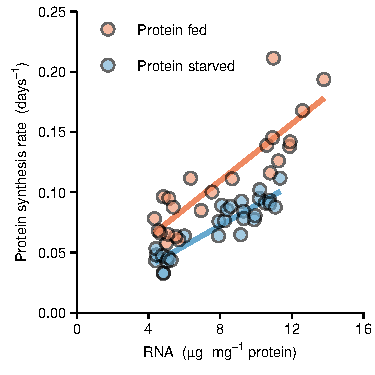
\includegraphics{thesis_files/figure-latex/Millward1973-1} 

}

\caption[Relationship between RNA content and protein synthesis in rat skeletal muscle, data from {[}164{]}]{Relationship between RNA abundance and protein synthesis in rat skeletal muscle. Rats were either starved or fed a protein rich diet stimulating protein synthesis. Data from {[}164{]}.}\label{fig:Millward1973}
\end{figure}
\hypertarget{mtorc1-a-multifaceted-coordinator-of-cell-growth}{%
\subsection{mTORC1 a multifaceted coordinator of cell growth}\label{mtorc1-a-multifaceted-coordinator-of-cell-growth}}

The discovery of an organic compound called rapamycin in the 1960's led to the characterization of a rapamycin sensitive protein involved in cell growth. The protein was later named mechanistic target for rapamycin (mTOR)
{[}165{]}.
mTOR is found in two protein complexes (mTOR complex 1, mTORC1; mTOR complex 2, mTORC2) where primarily mTORC1 has been found to be sensitive to rapamycin treatment
{[}165{]}.
Bodine \emph{et al.} performed a comprehensive characterization of mTORC1-mediated skeletal muscle hypertrophy using rodent models, showing that mTORC1 activation was essential for load-induced hypertrophy. Additionally, using transfection techniques, they showed that constitutively activated signaling upstream of mTORC1 (Akt) led to hypertrophy in an mTORC1-dependent manner, confirmed with concurrent administration of rapamycin
{[}166{]}.
Further utilizing rapamycin in genetically modified mice where mTOR was made rapamycin-resistant, specifically in skeletal muscle cells, confirmed that muscle-fiber specific rapamycin-sensitive mTORC1 signaling was needed to induce muscle hypertrophy in response to mechanical loading
{[}167{]}.
These mechanistic studies supports previous observational evidence connecting mTORC1 signaling to muscle growth in rats
{[}157{]},
and more recently, in humans
{[}20, 168{]}.

Administration of rapamycin in humans has also confirmed that mTORC1 signaling is important for protein synthesis in the acute phase after resistance training (2 hours) and in response to protein ingestion
{[}169, 170{]}.
However, extending the time-frame (up to 24 hours), differences in responses to resistance exercise between rapamycin treatment and control conditions were less pronounced
{[}171{]}.
This could in part be explained by the lower dosage of rapamycin administrated in human compared to animal trials but also indicate rapamycin-insensitive mechanisms controlling translational efficiency
{[}172, 173{]}.

mTORC1 functions as a signaling hub by integrating multiple environmental cues to regulate cellular growth. Among such cues is mechanical stimulation which leads to accumulation of phosphatidic acid in muscle cells
{[}174{]}.
Such accumulation was shown to be independent of regulators upstream of mTORC1 (phosphoinositide 3-kinase (PI3K)/AKT and ERK signaling)
{[}174, 175{]}
but still readily led to mTORC1 activation
{[}174, 175{]}.
In cellular models, phosphatidic acid has been shown to interact with mTORC1 on the same site targeted by rapamycin
{[}176{]}
indicating a more direct link between mechanical stimulation and mTORC1 activity.
The enzyme primarily responsible for mechanically induced increases of phosphatidic acid has been shown to be diacylglycerol kinase \(\zeta\)
{[}177{]}.

In the context of muscle growth in response to resistance training, adequate supplementation of dietary protein augments responses
{[}69{]}.
Mechanistically, dietary protein intake increase the availability of amino acids in muscle cells and these in turn stimulate protein synthesis through mTORC1 by multiple mechanisms
{[}178{]}.
mTORC1 capabilities to fine tune its response based on cellular status can be exemplified from studies examining responses to different amino acid compositions.
Providing a mixture of essential amino acids potentiated mTORC1 signaling in response to resistance exercise more than provision of essential amino acids without leucin or leucin alone
{[}179{]}.

In addition to mechanical stimuli and amino acids, mTORC1 integrate several environmental cues related to growth factors, energy and oxygen status with downstream signaling differing depending on upstream signaling and cellular characteristics
{[}180{]}.

Two downstream targets of mTORC1 rely much of the information related to translational control one of which is the well characterized eIF-4E (eukaryotic translation initiation factor 4E)-bining protein 1 (4E-BP1). Upon activation, 4E-BP1 releases eIF-4E
{[}181{]}
which enables formation of a preinitiation complex and subsequent recruitment of the small ribosomal subunit to mRNA
{[}182{]}.
eEIF-4E-dependent initiation of translation is believed to be rate limiting and thus a control point for protein synthesis.
Interestingly, formation of the preinitiation complex, induced by mTORC1-4E-BP1-mediated release of eIF-4E results in enhanced translation of special classes of mRNAs, containing a 5' structures that does not permit efficient translation
{[}182,183{]}.
Among the resulting gene products from such mRNA are growth factors, cell cycle regulators such as cyclin D1 and c-Myc as well as ribosomal proteins
{[}165,182{]}.

Parallell to 4E-BP1, is another well described downstream target of mTORC1, S6 kinase 1 (S6K1).
S6K1 was named after its ability to phosphorylate ribosomal protein S6, but has since been shown to have multiple roles related to both translational efficiency and indirectly to translational capacity
{[}165{]}.
The importance of S6K1 in control of muscle mass is apparent from S6K1 depletion in mice that results in reduces muscle growth and experiments showing that constitutevly active S6K1 resulting in increased myotube growth in cell cultures
{[}184, 185{]}.
S6K1 deficient mice did however not show a reduced translation of 5'TOP mRNA, an effect still sensitive to rapamycin
{[}186{]}.
Instead, S6K1 deficient mice have been shown to be unable to induce transcription of genes related to ribosomal biogenesis
{[}187{]}.
Upon activation of Akt, such mice fail to respond with increased ribosomal biogenesis, estimated through accumulation of total RNA and confirmed by targeted rRNA analysis
{[}188{]}.
S6K1 activity also leads to phosphorylation of downstream targets that enables translation initiation and elongation in addition to its most well known substrate ribosomal protein S6 (rpS6)
{[}189{]}.
Although a target of mTORC1, rpS6 have been shown to have conterintuitive role in protein synthesis.
Despite its location within the ribosome close to its core, mice genetically modified to be unable to phosphorylate rpS6 upon stimulation still form polysomes indicating that rpS6 phsophorylation is not needed for translational initiation
{[}190{]}.
Protein synthesis rates in the same mice are also higher compared to wild type mice suggesting an inhibitory role of rpS6 phosphorylation in protein synthesis
{[}190{]}.
Interestingly, mice depleted of S6K1 showed reduced specific force compared to wild-type mice, coinciding with forming of protein aggregates
{[}188{]}.
Together these observations points to fine-tuning mechanisms in the S6K1-rpS6-axis, balancing protein synthesis, protein quality and energy wastage
{[}188, 190{]}.
Fine-tuning may also exist within the mTORC1-S6K1 axis as S6K1 stimulates to mTOR phsophorylation at Ser\textsuperscript{2448}
{[}191{]},
a commonly used read-out for mTORC1 activity
{[}192{]}.
Additinally, mTORC1 signaling is sensitive to training status evident from changes in acute signaling in response to resistance training depending on the acute training status
{[}189, 193{]}.
After three and six weeks of training, the acute exercise-induced response (60-90 minutes post-exercise) in mTORC1-related signaling is practically abolished in young males
{[}193{]}.
Similarly, in well-trained participants accustom to resistance training, acute resistance-exercise does not lead to perturbations along the Akt-mTORC1-axis in comparison to endurance-trained participants
{[}194{]}.
These studies are limited in their temporal resolution as only signaling events in the early recovery phase were investigated.
However they indicate that exercise induced mTORC1-signaling is sensitive to aspects relating to training status.

\hypertarget{ribosomal-biogenesis-and-resistance-training-induced-muscle-hypertrophy}{%
\subsection{Ribosomal biogenesis and resistance training induced muscle hypertrophy}\label{ribosomal-biogenesis-and-resistance-training-induced-muscle-hypertrophy}}

The overall role of ribosomal abundance in determining protein synthesis and subsequent cellular and tissue size was briefly mentioned above.
In addition to correlations between RNA abundance and protein synthesis in mice
{[}164{]}
and cell culture
{[}195{]},
inhibition of ribosomal RNA (rRNA) transcription or inhibition of up-stream transcription factors act to diminish muscle cell growth upon stimulation
{[}196,195,197{]}.
In the context of resistance training-induced muscle growth, observational evidence from human studies further supports a determining role of ribosomal biogenesis to achieve increased translational capacity and enable hypertrophy.
Figueiredo \emph{et al.} observed a correlation between the changes in RNA abundance and magnitude of muscle growth over eight weeks of resistance training
{[}198{]}.
Stec and collegues observed increased ribosomal RNA and total RNA abundance only in participants that were classified as modest or extreme responders in terms muscle growth but not low responders after four weeks of resistance training
{[}196{]}.
Similarly, Mobley \emph{et al.} found larger increases in total RNA in participants classified as high- vs.~low-responders to 12 week resistance training (34\% vs.~8\% increase in total RNA) together with a correlation between total RNA increases and muscle growth over the same time period
{[}199{]}.
Finally, Reidy \emph{et al.} reported a correlation between changes in total RNA content and muscle growth
{[}160{]}
Together these studies underlines the importance of ribosomal biogenesis and translational capacity in resistance training-induced muscle hypertrophy.
It should be noted however, that protein synthesis and cellular growth may occur in the absence of ribosomal biogenesis.
In cultured myotubes stimulated with IGF-1, inhibition of ribosomal RNA transcription led to reduced RNA content but not myotube size compared to non-inhibited controls
{[}200{]}.
In aged male participants, three sessions of resistance training did not lead to increased levels of RNA but a 30\% increase in protein synthesis rates
{[}201{]}.
Furthermore, in response to a greater number of training sessions, absence or reduced ribosomal biogenesis are observed in selected individuals but muscle growth may still be detected
{[}193{]}.
However, when e.g.~comparing aged and young skeletal muscle, aged muscle typically respond with reduced hypertrophy after mechanical stimuli, coinciding with reduced ribosomal biogenesis
{[}193,202{]},
indicating that potent ribosomal biogenesis is needed to support greater hypertrophy.
Similarly, when comparing cell culture experiments, a ``broader'' stimuli induced by serum compared to a single growth factor could induce greater cellular growth that subsequently require support of an increased translational capacity
{[}200, 197, 196{]}.

Synthesis of ribosomes is indeed a hallmark of the early response to resistance training as a single resistance-exercise session leads to increases in precursor rRNA (pre-rRNA 45S)
{[}203,204{]}
and repeated bouts lead to accumulation of rRNA/total RNA and thus presumably functional ribosomes
{[}203, 205, 196,198, 193, 160{]}.
However, a time course of ribosomal transcription and accumulation in response to resistance training in humans remains largely unstudied.
Only a few studies have investigated exercise- or training-induced changes in markers of ribosomal abundance over multiple time-points.
For example, two consecutive bouts of electrically evoked muscle contractions were associated with increased levels of total RNA, with peak values being observed 72 hrs after the second bout
{[}205{]}.
Using voluntary contractions, peak values in total RNA were reported after nine sessions, followed by a slight decrease to after 18 sessions {[}193{]}.
These data suggest that ribosomes accumulates with some delay from initiation of training, reaches a plateau in the early phase of resistance training (three weeks) and slightly decreases as muscle mass further increases
{[}193,205{]}.

Synthesis of new ribosomes is a complex and energy demanding process. It involves the synthesis of both ribosomal proteins and four mature rRNA species as well as their assembly into functional ribosomal subunits
{[}206, 207,208{]}.
All mature rRNA (except rRNA 5S) are derieved from a single pre-rRNA transcript (45S pre-rRNA). After being transcribed from ribosomal DNA (rDNA), the 45S pre-rRNA transcript goes through several ``splitting'' events ultimately leading to the formation of three rRNA species, 18S, 5.8S and 28S. Coinciding with step-wise splitting of the pre-cursor transcript, modifications to the rRNA structure and assembly with ribosomal proteins into precursor ribosomal subunits occur in the nucleolar compartment
{[}207{]}.
After export to the cytoplasm, additional maturation steps are required in both subunits before they can form functional ribosomes\\
{[}207{]}.

Ribosomal biogenesis is believed to be determined by the rates of pre-rRNA transcription by RNA polymerase I (Pol I), which in turn is regulated by coordinated assembly of a complex of transcription factors at the rDNA promoter
{[}208{]}.
This process is co-regulated with translation as initiation of rDNA transcription is controlled by mTORC1 through multiple mechanisms.
Activation of the of the upstream binding factor (UBF) through phosphorylation is needed to initiate transcription
{[}209, 210{]}.
This activation is partly controlled by mTORC1 activity, with its inhibition being associated with blocked UBF phosphorylation and reduced UBF availability trough de-phosphorylation of retinablastoma protein.
This in turn leads to reduced availability and ability of UBF to recruit secondary factors to the rDNA promotor and stimulate rRNA transcription
{[}211, 212{]}.
mTORC1 also controls one of these secondary factors, TIF-1A, as rapamycin leads to specific phosphorylation and translocation away from the nuclei
{[}213{]},
in addition to inducing chromatin modulations at the rDNA promotor
{[}214{]}.

Parallell to mTORC1 control, specific inhibition of MEK showed that MEK/ERK signaling is important for UBF binding to rDNA
{[}215{]}.
Furthermore, the transcription factor c-Myc has also been implicated in ribosomal biogenesis as its inhibition coincides with less UBF activity and rRNA transcription irrespective of mTORC1 signaling
{[}195{]}.
c-Myc is also found at the rDNA promotor and is required for rDNA transcription
{[}216, 214{]},
in addition to its role in transcription of genes imoportant for rRNA transcription, e.g.~UBF
{[}217{]}.
Interestingly, the availability of UBF \emph{per se} has also been shown to be a determinant of rRNA transcription
{[}218, 212{]}
through control of rDNA gene activity
{[}219{]}.

In summary, ribosomal biogensis as well as the regulation of translation is under coordinated control of several pathways integrating multiple stressors and environmental cues to regulate cellular protein synthesis.

\hypertarget{transcriptional-regulation-of-training-induced-muscle-tissue-remodeling-with-analytical-challanges}{%
\subsection{Transcriptional regulation of training-induced muscle tissue remodeling (with analytical challanges)}\label{transcriptional-regulation-of-training-induced-muscle-tissue-remodeling-with-analytical-challanges}}

Skeletal muscle fibers are polynuclear cells. Each fiber contains multiple nuclei which supports its transcriptional requirements. Muscle fiber-specific nuclei (myonuclei) lack the ability to proliferate and are therefore relying on dormant cell populations located in muscle tissue to activate and supply the fiber with transcriptional capacity during growth or in response to injury
{[}220{]}.
Among these cells, satellite cells are the primary source of myonuclear accretion in adult skeletal muscle, however other cell types may also contribute
{[}220, 221{]}.
Satellite cells can activate, proliferate or differentiate and fuse with the muscle fiber upon specific stimuli such as hormonal activation
{[}222{]}
or mechanical stress
{[}223{]},
or return to their quiescent state
{[}220{]}
Satellite cells readily activates in humans in response resistance exercise by exiting their quiescent state to proliferate
{[}224, 225, 226{]},
leading to increased number of satellite cells after resistance training
{[}227{]}.

A possible growth limiting role for satellite cells in the context of muscle hypertrophy is to maintain a fixed number of myonuclei per muscle fiber volume through myonuclear accretion, in order to maintain transcriptional capacity (a maintained myonuclear domain)
{[}220{]}.
However, human studies are contradicting that such a role would be a determining factor for hypertrophy.
Kadi \emph{et al.} reported that although the number of satellite cells increased in response to training, the number of myonuclei did not,
suggesting that existing myonuclei were sufficient to provide transcriptional capacity in hypertrophied muscle
{[}228{]}.
Similarly, other studies have reported increases in muscle fiber cross-sectional area, without or with minimal concomitant enlargement of the myonuclei pool
{[}229, 230{]}.
In contrast, Petrella and colleagues reported that extreme responders to 16 weeks of resistance training also increased their myonuclear number more than modest and non-responders
{[}231{]}.
However, this analysis may have been confounded by the fact that the clustering did not account for age or sex. For example, the extreme-responder group contained 9 young (20-35 years) but only 2 elderly (60-75 years) male participants whereas the non-responder group contained 1 young man and 6 elderly
{[}232{]}.
This is of importance as satellite cell responses to exercise are different between young and elderly
{[}224{]}.
Using a similar clustering-approach as performed in {[}231{]} did not result in differences in myonuclear addition between different response-clusters in a homogeneous sample in terms of age (and sex)
{[}199{]}.
A further argument against the idea of a determining role of myonuclear addition in resistance-training induced hypertrophy comes from studies on mice where initial muscle growth induced by synergist ablation is unaffected by specific depletion of satellite cells
{[}221{]}.

In humans, addition of myonuclei paralleled with an increase in global transcription rates from existing myonuclei are likely both contributing to accumulation of total RNA seen after resistance training.
Myonuclear accretion does not, however, seem to be a limiting factor for muscle growth
{[}199, 221{]}.
Existing myonuclei are thus able to maintain transcriptional requirements during hypertrophy, possibly relating to a large degree of transcriptional reserve capacity in muscle fibers
{[}233{]}.
Indeed, this reserve capacity of existing myonuclei seems sufficient to induce a global shift in transcription in response to mechanical loading, including both mRNA and rRNA transcription
{[}234{]}.
Such a shift in global transcription is indeed a determinant of muscle growth as it sets the limit of ribosomal biogenesis and thus the muscle cells translational capacity (as reviewed above).

A change in transcription in response to mechanical loading is not only quantitative (RNA per unit of tissue mass) but also qualitative (changed profiles among e.g.~mRNA) in nature with multiple transcriptional programs enabling coordinated adaptation to the specific stimuli.
Such ``programming'' in muscle tissue affects e.g.~muscle fiber type composition where resistance training leads to ``shut-down'' of \emph{MYH1}, coding for the myosin isoform represented in type IIX fibers
{[}100{]}.
The changed, relative proportions of transcripts coding for myosin composition will after remodeling reflect the resulting phenotype
{[}101{]}.
Furthermore, transcriptional remodeling of the extracellular matrix is readily affected by resistance training
{[}235, 119{]}.
Revisiting the role of satellite cells, briefly touched upon in a previous paragraph, highlights that transcriptional regulation of muscle remodeling is a shared venture between multiple cell types when it comes to the extracellular matrix.
If satellite cells are depleted from skeletal muscle of mice subjected to long-term mechanical overload through synergist ablation, a fibrous muscle phenotype is developed with accumulated extracellular matrix components
{[}236{]}.
Balance between muscle satellite cells, their daughter cells and fibroblasts enables coordination between myofiber hypertrophy and extracellular matrix remodeling
{[}236, 237, 116{]}.
Such coordinated remodeling occurs at least partly through direct exosome transfer of regulating RNA between differentiated satellite cells and fibroblasts
{[}237{]}.

In humans, previous studies relating to resistance training and muscle growth/function have investigated a single resistance-exercise session {[}235, 119, 238{]},
repeated bouts
{[}239{]}
and chronic resistance training {[}240, 119, 235, 120{]}
for changes in transcriptome (``qualitative'') characteristics using large-scale techniques (micro-arrays or RNA-seq).
Generally, these studies show that a bout of resistance exercise in the untrained state results in a transcriptome profile related to structural damage, remodeling and inflammation
{[}239{]}.
Long term adaptations generally involves extracellular matrix remodeling, changes expression of genes related to energy metabolism\\
{[}240, 119, 235, 120{]}.
Attempts have also been made to associate transcriptome characteristics and degrees of muscle growth
{[}120, 55, 241{]},
and muscle function
{[}242, 243{]}.

Although these studies have broaden our understanding of transcriptional regulation during adaptations to resistance training, they also highlight the intrinsic difficulties in studying a dynamic and stochastic process
{[}233{]}.
From a methodological point of view, skeletal muscle subjected to e.g.~resistance training, concomitant with muscle hypertrophy both exhibit large global scale changes to the RNA pool as well as important \emph{qualitative} changes to RNA sub-populations (mRNA).
A common assumption in studies of gene expression is the relative stability of most transcripts, as well as stability between sub-populations of RNA (mRNA vs.~rRNA)
{[}244, 245{]}.
Such assumptions may not be true in many situations, including during muscle hypertrophy
{[}234, 246, 196, 198, 193{]}.
Depending on the technique used for evaluating RNA expression (e.g.~qPCR, micro-array or RNA-seq), data normalization during analysis aims to make experimental conditions comparable using some common denominator.
In cell culture experiments, cell number was suggested to be this denominator for transcript abundances in order to account for global changes in transcription
{[}244{]}.
Despite the fact that some previous investigations, specifically investigating resistance training, have acknowledged a changed total RNA abundance per muscle weight, indicating that a lower amount of tissue being used in analysis in different conditions (trained vs.~untrained muscle)
{[}119{]},
transcript counts are commonly expressed as per transcriptome.

In summary, both quantitative and qualitative changes in transcriptional profiles determines the cellular phenotype. Skeletal muscle hypertrophy may represent a special case in studies of transcriptome characteristics as it is typically associated with global changes in transcription as well as cellular growth. To fully understand such dynamic systems, first steps should include explicit evaluation of underlying assumptions
{[}247, 244, 248{]}

\hypertarget{effects-of-exercise-volume-on-molecular-determinants-of-muscle-growth}{%
\section{Effects of exercise volume on molecular determinants of muscle growth}\label{effects-of-exercise-volume-on-molecular-determinants-of-muscle-growth}}

Given that exercise-training variables can modify responses to resistance training, it is reasonable to assume that these effects are mediated through determinants of muscle growth.
Exercise intensity has been evaluated with respect to protein synthesis and activation of targets downstream of mTORC1 (4E-BP1 and S6K1).
Kumar \emph{et al.} showed that maximal stimulation of fractional synthetic rate was achieved with intensities greater than 60\% of 1RM, coinciding with signaling events
{[}249{]}.
The same group subsequently investigated the effect of training volume at an intensity presumably leading to maximal stimulation of protein synthesis (75\% of 1RM).
This analysis revealed a volume-dependent dose-response as six-sets of leg extension led to greater protein synthesis one hour after exercise and sustained S6K1 phsophorylation over up to four hours after exercise
{[}250{]}.
Further extending the time frame, Burd and colleagues evaluated a single session consisting of either one or three sets with biopsies sampled 5, 24 and 29 hour after exercise. Both conditions led to increased myofibrillar protein synthesis five and 29 hours after exercise, but to a larger extent in response to three sets.
However, volume-dependent regulation of S6K1 was only seen at 29 hours after exercise with earlier events (\textless{} 5 hours) possibly missed due to the timing of biopsy sampling.
No clear volume-dependency was seen in p90RSK1 (downstream of ERK) or rpS6, however eukaryotic initiation factor 2B (eIF2B\(\epsilon\)) phosphorylation was reduced only in the three set condition at five hours post exercise {[}20{]}, presumably mediating translation initiation, although its exact role is still unclear
{[}251{]}.
Volume dependent regulation of S6K1 at Thr389 and rpS6 at Ser235/236 were reported 30 minutes after exercise by Terzis \emph{et al.} as six sets of 6RM bilateral legpress resulted in greater phosphorylation compared to three and one set
{[}21{]}.
No clear differences between volume conditions were seen in Akt at Ser473, mTOR at Ser2448, ERK 1/2 at Thr202/Tyr204, p38 (\(\alpha\),\(\alpha\) and \(\delta\)) at Thr180/Tyr182, p38\(\gamma\) Thr180/Tyr182 or AMPK at Thr172
{[}21{]}.
Corroborating previous observations regarding exercise volume-dependence of the S6K1-rpS6-axis, Ahtiainen and colleagues also found greater phosphorylation of S6K1 at Thr389, rpS6 at Ser235/236 and Ser240/244 30 minutes after exercise with ten compared to five sets of 10RM legpress.
Furthermore, ERK1/2 at Thr202/Tyr204 and p38 at Thr180/Tyr182 phosphorylations were not found to be volume dependent
{[}22{]}.
However, in contrast to Terzis \emph{et al.}, they reported volume-dependence in exercise-induced phsophorylation of AMPK\(\alpha\) at Thr172, this together with AS160 at Thr642, IRS-I Ser636/639 and Akt at Ser473 together with a tendency in LKB1 at Ser428, all related to cellular energy status, glucose uptake and metabolism
{[}22,252{]}

Collectively, although limited in precision due to small sample sizes (n = 8-19) and temporal resolution and
these studies points to volume dependency in exercise-induced S6K1\textsuperscript{Thr389} phosphorylation, potentially further augmented when increased number of sets are examined in the acute phase
(\textgreater{} 3 sets, \textless{} 5 hours; {[}20,146{]} vs. {[}21,22,250{]}).
Increased S6K1 phosophorylation coincides with rpS6\textsuperscript{Ser235/236} and \textsuperscript{Ser240/244} in the acute phase (\textless{} 5 hours) after exercise
{[}21,22{]} but not in the late phase (29 hours) {[}20{]}.
Although rpS6\textsuperscript{Ser235/236} is a known substrate for both S6K1 and ERK1/2 and p90RSK1
{[}253{]},
ERK1/2\textsuperscript{Thr202/Tyr204} was not been found to be volume-sensitive in the acute phase
{[}21,22{]},
nor was P90RSK1\textsuperscript{Thr573} in the late phase {[}20{]}
suggesting that signaling along the mTORC1-S6K1-rpS6-axis is more sensitive to variable volume than the parallell MEK/ERK-axis.
The above signaling events suggest exercise volume-dependent activation of the translational machinery, and increased volume indeed leads to increased muscle protein synthesis
{[}20,250{]}.
However, relatively high exercise volumes may lead to signaling events inhibiting protein synthesis as AMPK\textsuperscript{Thr172} showed volume dependency, presumably relating to cellular energy stress and glucose metabolism
{[}22,252, 254{]}.
Interestingly, an increased AMPK-related signaling may be related to an accumulated effect due to short inter-set rest periods, coinciding with reduced proteins synthesis, at least in the acute phase after exercise
{[}255{]}.

In addition to the signaling events described above, training-induced satellite cell activation has been shown to be volume dependent.
Hanssen \emph{et al.} found that training with three sets compared to a single-set per exercise led to more pronounced increase in cells positive for the satellite cell marker CD56 in \emph{m. vastus lateralis} at two and twelve weeks of resistance training {[}256{]}.
This coincided with a greater number of myonuclei after 12 weeks of training, however with no clear differences between volume conditions.
In the same muscle specimen, no clear volume-dependent effect was seen on muscle fiber CSA, however on the muscle level a positive effect of three- compared to one-set was seen for muscle hypertrophy.
{[}145,256{]}

\hypertarget{aims}{%
\chapter{Aims}\label{aims}}

The primary aim of this thesis was to relate the adaptive response to resistance training with low- and moderate-volume to skeletal-muscle characteristics in previously untrained individuals. The key question was whether manipulation of exercise-volume will have diverse effects in different individuals related to muscular intrinsic characteristics. A further aim was to characterize exercise-volume dependence in muscle molecular characteristics and determine a time course profile of markers of ribosomal biogenesis in response to resistance training. Based on these aims, the objectives of the present thesis were;
\begin{itemize}
\tightlist
\item
  to relate skeletal muscle and systemic characteristics to benefit of moderate- compared to low-volume resistance training;
\item
  To determine volume-dependence in molecular networks related to muscle growth and remodeling in response to resistance training
\item
  To determine a time course of markers related to ribosome biogenesis in the early phase of resistance training.
\end{itemize}
\hypertarget{methods}{%
\chapter{Methods}\label{methods}}

\hypertarget{study-overview}{%
\section{Study overview}\label{study-overview}}

Study I was designed to examine effects of low- (a single-set per exercise) and moderate-volume (three sets per exercise) on responses to acute exercise and long-term training within participants.
A schematic overview of Study I can be seen in Figure \ref{fig:study1-overview}.
Prior to the training intervention, participants reported to the laboratory for bilateral baseline muscle biopsies (\emph{m. vastus lateralis}).
Bilateral muscle biopsies were additionally sampled prior to, and 60 minutes after the fifth training session as well as after the intervention (Figure \ref{fig:study1-overview}).
Assessments of muscle strength (unilateral isokinetic and isometric knee extension torque as well as unilateral knee extension and leg press one repetition maximum) were performed twice at baseline and further measured in weeks 3, 5, 9 and after the intervention (Figure \ref{fig:study1-overview}).
Body composition measurements (magnetic resonance imaging and dual-energy X-ray absorptiometry) were performed at baseline and after the intervention.

Study II was designed to study the effects of resistance training \emph{per se} and effects of variable compared to constant inter-session volume on selected markers related to ribosome biogenesis.
Participants were therefore recruited to an experimental group and a non-training control group.
An overview of Study II can be seen in Figure \ref{fig:study2-overview}.
Baseline muscle strength (unilateral isokinetic and isometric knee-extension torque) was assessed during three initial visits to the laboratory, with the last baseline-assessment performed at least seven days prior to the first biopsy sampling. Follow-up measures of muscle strength in the experimental group were completed three and nine days after the last training session.
Muscle thickness (\emph{m. vastus lateralis}) was measured bilaterally prior to the study as well as two and eight days after the last training session in the experimental group.
Muscle biopsies were sampled bilaterally prior to any training, 48 hours after the first, fourth, fifth, eighth, ninth and twelfth session as well as eight days after the twelfth session (Figure \ref{fig:study2-overview}).
The control group in Study II performed the same initial assessments as the experimental group. Muscle thickness was again assessed after a control period of 2-4 weeks.
Follow-up muscle biopsies were sampled from one leg 48 hours after the first biopsy as well as after the control period. Follow-up strength assessments were performed 24 hours after the last biopsy.
\begin{figure}

{\centering 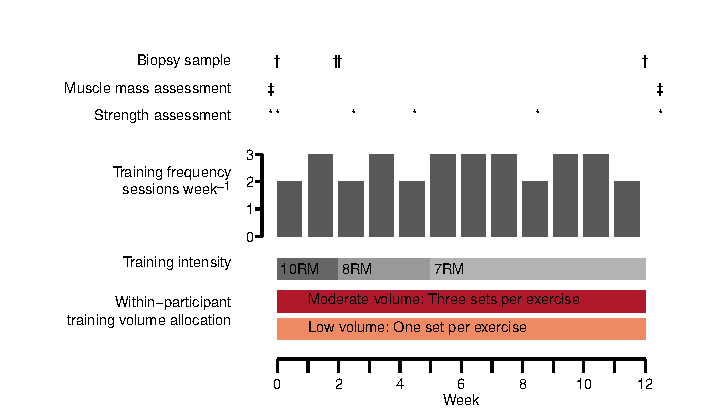
\includegraphics{thesis_files/figure-latex/study1-overview-1} 

}

\caption[Study I, schematic overview]{Schematic representation of Study I, see text for details.  }\label{fig:study1-overview}
\end{figure}
\begin{figure}

{\centering 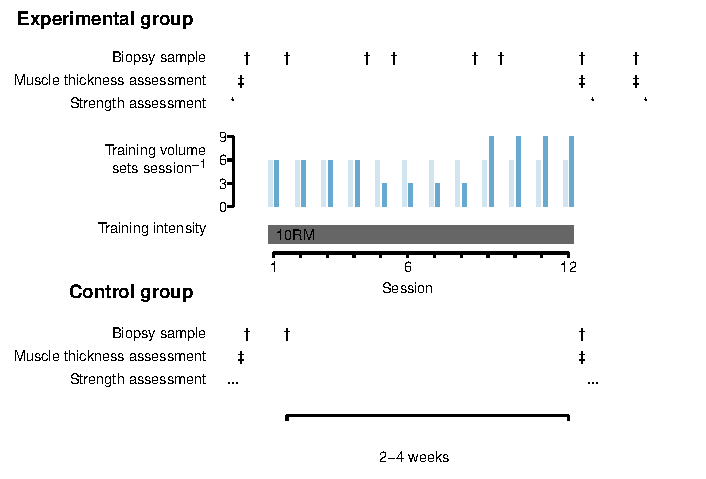
\includegraphics{thesis_files/figure-latex/study2-overview-1} 

}

\caption[Study II, schematic overview]{Schematic representation of Study II, see text for details.  }\label{fig:study2-overview}
\end{figure}
\hypertarget{participants}{%
\section{Participants}\label{participants}}

Recruitment to both studies was done through advertising and word of mouth, primarily at Lillehammer University College/Inland University of Applied Sciences. Potential participants were interviewed and matched against inclusion and exclusion criteria. During initial interviews, participants were informed of the study design and time requirements. Participants were also informed about potential risks and sources of discomfort associated with the study prior to giving their informed consent.

To be eligible for participation in both studies, participants had to be young (Study I age 18-40; Study II 18-35) and non-smoking. Both men and women were considered for participation. Exclusion criteria included a training history of more than one weekly session during the last 12 (Study I) or six (Study II) months leading up to the study. Participants were also screened for intolerance to local anesthetic, current or previous injuries affecting their ability to perform resistance training, self-reported symptoms or history of disease, intake of medications or supplements with known effects on adaptations to training.
Participant characteristics for both studies are shown in Table
\ref{tab:characteristics-table}.

Forty-one participants were recruited to Study I and 34 of these completed at least 85\% of the prescribed sessions and were thus included in subsequent data analyses. Reasons for not completing the trial included injury not related to the study (\emph{n =} 1), pain or discomfort during exercises (\emph{n =} 5) and non-adherence to the study protocol (\emph{n =} 1). There were no systematic differences in characteristics between participants included in or excluded from data analysis in Study I. Prior to the study, all participants reported that they had previously been engaged in sporting activities. At enrollment, twenty participants reported regular physical activities ranging from once every other week to four times per week. Ten participants reported performing resistance-type exercise at the time of enrollment limited to no more than once a week.

Twenty-two participants were recruited to Study II. Three participants did not complete the intervention due to scheduling difficulties. Participants reported familiarity with physical activity but no current systematic strength training.
\begin{landscape}\begin{table}

\caption{\label{tab:characteristics-table}Participant characteristics}
\centering
\fontsize{7}{9}\selectfont
\begin{tabular}[t]{lllrlllll}
\toprule
  &   & Sex & n & Age (years) & Stature
(cm) & Mass (kg) & Fat mass (\%) & Lean mass (\%)\\
\midrule
 &  & Female & 18 & 22.0 (1.3) & 168 (7) & 64.4 (10.4) & 34.1 (5.6) & 64.3 (6.2)\\
\cmidrule{3-9}
 & \multirow{-2}{*}{\raggedright\arraybackslash Included} & Male & 16 & 23.6 (4.1) & 183 (6) & 75.8 (10.7) & 20.4 (6.0) & 79.3 (5.0)\\
\cmidrule{2-9}
 &  & Female & 4 & 22.9 (1.6) & 166 (8) & 64.6 (9.7) & 28.8 (8.7) & 68.6 (9.1)\\
\cmidrule{3-9}
\multirow{-4}{*}{\raggedright\arraybackslash Study I} & \multirow{-2}{*}{\raggedright\arraybackslash Excluded} & Male & 3 & 24.3 (1.5) & 189 (5) & 88.2 (22.4) & 24.3 (15.3) & 76.8 (12.7)\\
\cmidrule{1-9}
 &  & Female & 6 & 23.4 (2.9) & 168 (8) & 64.0 (9.2) & 30.8 (7.1) & 65.5 (6.8)\\
\cmidrule{3-9}
 & \multirow{-2}{*}{\raggedright\arraybackslash Training} & Male & 5 & 25.7 (5.8) & 177 (3) & 77.5 (8.0) & 25.3 (3.9) & 71.3 (2.4)\\
\cmidrule{2-9}
 &  & Female & 4 & 24.1 (3.5) & 166 (4) & 63.8 (0.6) & 30.5 (6.4) & 66.3 (5.2)\\
\cmidrule{3-9}
\multirow{-4}{*}{\raggedright\arraybackslash Study II} & \multirow{-2}{*}{\raggedright\arraybackslash Control} & Male & 4 & 25.5 (5.5) & 182 (5) & 76.5 (7.7) & 18.2 (5.1) & 78.7 (4.2)\\
\bottomrule
\multicolumn{9}{l}{\rule{0pt}{1em}Data are means and (SD)}\\
\end{tabular}
\end{table}
\end{landscape}
\hypertarget{ethical-approvals}{%
\subsection{Ethical approvals}\label{ethical-approvals}}

Both studies were conducted according to the Declaration of Helsinki
{[}257{]}.
Studies were approved by the local ethics committee (Study I, no. 2013-11-22:2; Study II, no. 2017-10-23), the Norwegian centre for research data (Study I, 36930/3/LB; Study II, 51549/3/AH) and pre-registered (Study I, ClinicalTrials.gov Identifier: NCT02179307; Study II, DOI 10.17605/OSF.IO/WA96Y).

\hypertarget{resistance-training-interventions}{%
\section{Resistance training interventions}\label{resistance-training-interventions}}

Studies were fully or partially performed as within-participant studies
as each participant had their legs assigned to different training
conditions (not including the control group in Study II). Allocation was
performed after enrollment where each participant had their legs
randomized to either low- or moderate volume (Study I, see Figure \ref{fig:study1-overview}), or variable or constant volume (Study II).

Each training session started with a light, standardized warm-up (5 min
ergometer cycling and 10 repetitions each of push-ups, sit-ups,
back-extensions and squats). Before each exercise in the main program,
one set of 10 repetitions were performed in the specific exercise with
approximately 50\% of 1RM.

In Study I, the low-volume protocol consisted of a single set of each
exercise and the moderate-volume program consisted of three sets per exercise.
Three unilateral leg exercises were used (leg press, leg curl and knee
extension). The moderate-volume leg commenced all sessions and the low-volume leg performed a single set of each exercise in the rest between
second and third set of the moderate volume training protocol.

In Study II, only unilateral knee-extension was performed. The constant-volume leg performed six sets of 10RM throughout the study and variable leg performed six sets in session one to four, three sets in session five to eight and nine sets in session nine to twelve with same relative intensity (see Figure \ref{fig:study2-overview}).

In both studies, participants perfomed leg-exercise as part of a full-body program with upper-body exercise performed with two sets after leg-exercises. Upper-body exercises included bilateral bench-press, pull-down, and either shoulder-press or seated rowing.

\hypertarget{muscle-strength-assessments}{%
\section{Muscle strength assessments}\label{muscle-strength-assessments}}

Strength was assessed as one repetition maximum (Study I), isometric and isokinetic torque (Study I and II). In Study I, maximal values from each assessment and time-point were used in statistical analyses including two separate assessments at baseline, separated by at least four days. A combined muscle strength index was calculated as the average of all tests (1RM, isometric and isokinetic), with all test types given equal weight (expressed as \(\frac{x_i}{max(x)}\) where x is a strength measure for each leg and time-point (\(i\))). Eighteen participants performed strength assessments at week two, five and nine in addition to baseline and post-training assessments. Training sessions were prioritized for the remaining participants when illness or scheduling difficulties prevented both strength assessment and training.

In Study II, the maximal value from all successful attempts were used in statistical analyses with unsuccessful attempts identified based on obvious misinterpretation of instructions or failure to reach maximal subjective effort. Strength assessments were separated by at least 48 hours from preceding training sessions.

\hypertarget{isokinetic-and-isometric-maximal-torque}{%
\subsection{Isokinetic and isometric maximal torque}\label{isokinetic-and-isometric-maximal-torque}}

Maximal isokinetic and isometric unilateral knee-extension strength was determined by use of a dynamometer (Study I: Cybex 6000, Cybex International, Medway USA; Study II: Humac Norm, CSMi, Stoughton, MA, USA).
After a brief warm-up (5 min ergometer cycling, RPE 12-14), participants were secured at the hip and shoulders in the dynamometer with the knee joint aligned to its rotation axis.
Individual settings were recorded and used in subsequent measurements.
Participants were familiarized with the test protocol by performing three sub-maximal efforts at each angular speed.
In Study I, three angular velocities were used to determine isokinetic torque (60\(^{\circ}\), 120\(^{\circ}\) and 240\(^{\circ} ~\times\) sec\(^{-1}\)), in Study II an angular velocity of 90\(^{\circ} ~\times\) sec\(^{-1}\) was used for this purpose.
In Study I, participants performed two attempts at 60\(^{\circ} ~\times\) sec\(^{-1}\) and three attempts at 120 and 240\(^{\circ}~\times\) sec\(^{-1}\).
In Study II, three attempts were made at the designated angular velocity.
In both studies, attempts within each angular speed were performed in immediate succession.
After isokinetic testing, the lever was fixed at 30\(^{\circ}\) (full extension \(=90^{\circ}\)), participants were instructed push with maximal effort for 5 seconds and the maximal isometric torque was recorded.
Two attempts were made for maximal isometric torque in Study I and a single attempt was made in Study II.
Sixty seconds of restitution was given between each measurement in both studies with the exception of between isometric contractions in Study I where a 30 second restitution period was used.

In subsequent assessment sessions, the first measurement was performed on alternate legs.
In Study II, the dynamometer allowed for participants to remain seated for assessments of both legs. This was not possible in Study I as the measurement system required participants to be re-seated for assessment of the contra-lateral leg.

\hypertarget{one-repetition-maximum}{%
\subsection{One-repetition maximum}\label{one-repetition-maximum}}

One repetition-maximum (1RM) was assessed in unilateral leg-press and knee-extension in Study I.
Each exercise was assessed after a specific warm-up (ten, six and three repetitions at \(50\), 75 and \(85\%\) of the anticipated maximum). Attempts were made with increasing resistance (four to six attempts) and one repetition maximum was defined as the highest resistance successfully lifted through the full range of motion.

\hypertarget{measures-of-muscle-mass}{%
\section{Measures of muscle mass}\label{measures-of-muscle-mass}}

In Study I muscle mass was measured by magnetic resonance imaging (MRI)
and dual energy X-ray absorptiometry (DXA) prior to and after the
intervention. Both MRI and DXA measurements were completed during the
same visit to the laboratory. Participants were instructed to refrain
from strenuous physical activity during the last 48 h leading up to the
measurements. The post-training measurements were completed at least 48
h after the last strength testing session. Participants were asked to
refrain from food consumption during 2 h leading up to the measurements.

MRI images were obtained from the mid-thigh and analyzed by the same
investigator blinded for time (pre- and post-training) and condition
(low- and moderate-volume). Multiple images were used to estimate the
cross-sectional area of the extensor muscles at the same distance from
the knee-joint.

In Study II, \emph{m. vastus lateralis} muscle thickness was measured by B-mode ultrasonography (SmartUs EXT-1M, Telemed, Vilnius, Lithuania) using a 39 mm 12 MHz, linear array probe. Between each image acquisition the probe was relocated to the same position. The position was marked on a soft transparent plastic sheet used to relocate the same position in subsequent measurements.
At least three images were captured and quantified for each leg per time-point with values averaged in analyses. Images were analyzed in ImageJ Fiji {[}258{]} by a single assessor blinded for study conditions and time-points.

\hypertarget{muscle-tissue-sampling-and-preparations-for-downstream-analyses}{%
\section{Muscle tissue sampling and preparations for downstream analyses}\label{muscle-tissue-sampling-and-preparations-for-downstream-analyses}}

Muscle samples were obtained under local anesthesia (Study I, Xylocaine,
\SI{10}{\mg\per\ml} with adrenalin \SI{5}{\micro\gram\per\ml},
AstraZeneca, Oslo, Norway; Study II, Lidocaine Mylan,
\SI{10}{\mg\per\ml}, Mylan Ireland Ltd, Ireland) with a fine needle
(12-14 gauge; Universal-plus, Medax, Italy) operated with a
spring-loaded instrument (Bard Magnum, Bard Norway AS, Norway).
Sampling was performed as previously described
{[}259{]}, with
modifications. Anesthesia was injected in the subcutaneous tissue with
care taken not to inject anesthesia into the muscle itself. Following
pilot experiments we decided not to use an insertion cannula as
described in {[}259{]} as the biopsy needle itself could be used to
puncture the skin and muscle fascia. This also resulted in less
discomfort. Several passes through the same skin puncture was made to
obtain sufficient material for downstream analyses. A smaller needle (14
vs.~12 gauge) was used to further minimize discomfort in Study II where
more biopsies were sampled over a shorter time span, with exception from
when material was used for immunohistochemistry. The first biopsy was
sampled at one third of the distance between the patella to the
\emph{anterior superior iliac spinae} with subsequent biopsies sampled
\(\sim\)\SI{2}{cm} proximal to previous samples. In Study II, samples
obtained more than one week apart were sampled with closer proximity and
distally from previous samples but never at previous sampling sites.

\hypertarget{immunohistochemistry}{%
\subsection{Immunohistochemistry}\label{immunohistochemistry}}

In Study I, a portion of each sample was selected for immunohistochemistry analysis. Samples were placed in formalin for fixation (2-4 days) and further processed using a Shandon Excelsior ES (2.5 hours, Thermo Scientific, USA). Samples were sectioned in \SI{4}{um} transverse sections. Orientation was confirmed prior to subsequent specific staining. In case of obvious misalignment, samples were re-oriented and sectioned. Muscle fiber types were determined on sections double-stained with BF-35 (\SI{5}{\micro\gram\per\milli\litre}, Developmental Studies Hybridoma Bank, deposited by Schiaffino, S.) targeting all both myosin heavy-chain Type I and Type IIA, and MyHCSlow (1:4000, catalog M8421L, Sigma-Aldrich Norway AS, Oslo, Norway) specifically targeting myosin heavy-chain Type I.
Antobodies were visualised using BMU UltraView DAB (BF-35) and UltraView Red (MyHCSlow, Ventana Medical Systems, Inc.~Tucson, USA).
Muscle fibers were counted as Type I (red), Type IIA (brown), Type IIX (unstained) or Type IIA/IIX hybrid fibers (light-brown, see Figure \ref{fig:myhc-fig}). Hybrid fibers were analyzed as 0.5 \(\times\) Type IIA and 0.5 \(\times\) Type IIX
{[}101{]}.

\hypertarget{total-rna-extraction}{%
\subsection{Total RNA extraction}\label{total-rna-extraction}}

Total-RNA was extracted from frozen muscle samples with weights measured at collection using a protocol modified from
{[}260{]}
using Trizol reagent (Life Technologies).
Muscle tissue was homogenized in \SI{300}{ul} Trizol with mechanical disruption achieved by Zirconium Oxide Beads (0.5 mm, Next Advance, Inc., New York, USA) and a bead mill (Bullet blender, Next Advance). External, non-mammalian RNA (Lambda PolyA External Standard Kit, Takara Bio Europe, Saint-Germain-en-Laye, France) was added with the initial volume of Trizol to enable per-weight normalization in subsequent analyses. After homogenization, additional Trizol was added to a total volume of \SI{1}{ml}. Phase separation was achieved by centrifugation after addition of chloroform (\SI{200}{ul}). The upper phase (\SI{400}{ul} in Study I; \SI{450}{ul} in Study II) was transferred to a fresh tube and RNA was precipitated using isopropanol (\SI{500}{ul}). After incubation (10 min, room-temperature) and centrifugation (12000 g, 10 min at 4\(^{\circ}\)C) the resulting RNA pellet was washed three times in chilled 75\% ethanol.
\begin{figure}

{\centering 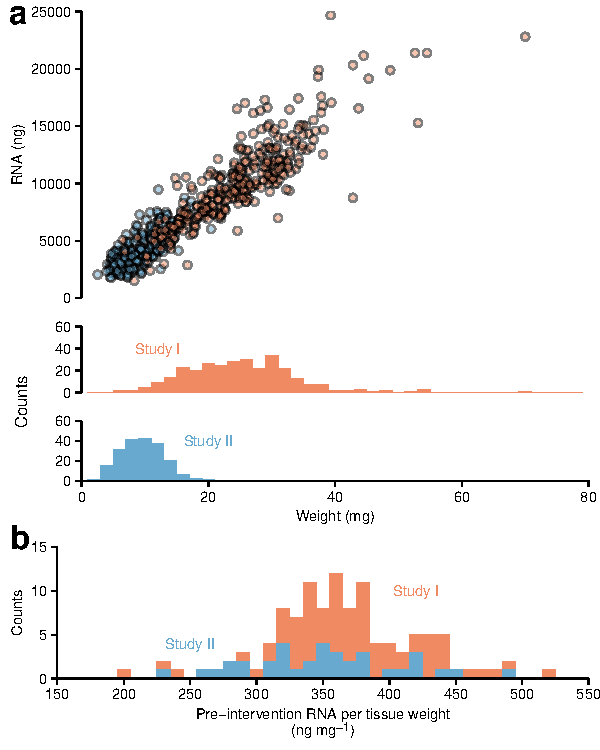
\includegraphics{thesis_files/figure-latex/rna-muscle-weight-methods-1} 

}

\caption[Characteristics of total RNA extracted per study]{Characteristics of total RNA extracted per study and relationship with muscle weight (a). Distribution of pre-intervention RNA per tissue weight (ng mg\textsuperscript{-1}) (b)}\label{fig:rna-muscle-weight-methods}
\end{figure}
As previously mentioned, to minimize discomfort due to a greater number of biopsies sampled over a short time, a smaller needle was used for most biopsies in Study II. This generally led to a less tissue used for RNA extractions, however, samples from both studies followed the same association between sample weight and Total RNA content (Figure \ref{fig:rna-muscle-weight-methods}a). Further comparing studies using pre-intervention biopsies indicate comparable RNA per tissue-weight readings across the two studies (Figure \ref{fig:rna-muscle-weight-methods}b).

\hypertarget{protein-extraction-and-immunoblotting}{%
\subsection{Protein extraction and immunoblotting}\label{protein-extraction-and-immunoblotting}}

In Study I, muscle-tissue (\(\sim\) \SI{25}{mg} wet weight) was homogenized using a plastic pestle in ice-cold lysis buffer (2 mM HEPES pH 7.4, 1 mM EDTA, 5 mM EGTA, 10 mM MgCl\textsubscript{2}, 1\(\%\) Triton X-100) supplemented with protease and phosphatase inhibitors (Halt, Thermo Fischer Scientific, Life Technologies AS, Oslo Norway). Samples were subsequently incubated at \(4^{\circ}\) for 1 hour followed by centrifugation (10 min at 10 000 g and 4\(^{\circ}\)C). Supernatants were collecetd used for total protein quantification using Bradford reagents (Pierce Detergent Compatible Bradford Assay Reagent, Thermo Fischer Scientific).
Samples were normalized in lysis buffer and 4X Laemmli sample buffer (Bio-Rad Laboratories AB, Oslo Norway) containing 2-Mercaptoethanol, heated to 95\(^{\circ}\)C for 5 min and stored at -20\(^{\circ}\)C until further processing.

In Study II, protein was extracted from Trizol preparations according following suggestions by Kopec \emph{et al.} {[}261{]}
with modifications. After remiving the remaining aqueous phase, DNA was precipitated by addition of \SI{300}{ul} of absolute ethanol and centrifugation (2000 g, 5 min at room temperature). An aliquot of the phenol-ethanol phase, corresponding to \(\sim\) \SI{1.75}{mg} of tissue, was transferred to to a fresh tube and at least two volumes of isopropanol were added followed by incubation (10 min at room temperature). After centrifugation, (7500 g, 10 min 4\(^{\circ}\)C) a pellet formed and was subsequently washed three times in 95\% ethanol. Each wash was separated by centrifugation (5000g, 5 min at room temperature). Following the final wash, all liquid was removed and \SI{45}{ul} of Kopec buffer {[}261{]} was added (5\% SDS, 10 mM Tris, 140 mM NaCl and 20 mM EDTA, pH 8; containing protease and phosphatase inhibitors).
Pellets were incubated three hours at 50\(^{\circ}\)C after which nearly all samples were dissolved.
Any undissolved material was sedimented by centrifugation (10000 g, 10 min at room temperature).
Protein concentrations were determined and samples normalized as described for Study I.

In both studies, \SI{20}{ug} total protein per sample was separated by gel eletrophoresis (250-300 V for 30-50 min using 4-20\% gels, Criterion TGX, Bio-Rad), and transferred to PVDF membranes (300 mA for 3 h, \SI{0.2}{um} Immun-Blot, Bio-Rad).
Membranes were stained for total protein using a reversible total protein stain (Pierce Reversible Protein Stain, ThermoFischer Scientific) to ensure transfer and enable protein quantification.
Membranes were blocked for 2 h in blocking buffer (tris-buffered saline, TBS, 20 mM Tris, 150 mM NaCl) containing \(3\%\) bovine serum albumin or 5\% skimmed milk and \(0.1\%\) Tween-20.
Incubation with primary antibodies were done over-night followed by 1-2 hours incubation with secondary antibodies.
Membranes were washed in TBS containing \(0.1\%\) Tween-20 for 3-8 \(\times\) 5-10 min after incubation with primary antibody, and for 4-8 \(\times\) 5-10 min after incubation with secondary antibodies.
Chemiluminescent detection was used to quantify relative target protein abundance (SuperSignal™ West Femto Maximum Sensitivity Substrate, ThermoFischer Scientific).
For selected targets, following chemiluminescent detection, membranes were incubated with hydrogen peroxide (15 min, 37\(^{\circ}\)C) to inactivate the horseradish peroxidase (HRP), as described by Sennepin \emph{et al.} {[}262{]}, enabling detection of other epitopes using antibodies from different hosts (mouse or rabbit).
Incubation and wash steps were either performed in an automated fashion at \(4^{\circ}\)C (BlotCycler, Precision Biosystems, Mansfield, MA, USA), or by hand at room temperature with incubations at \(4^{\circ}\)C.
Total-protein content, defined as the mean grey value of the whole well was quantified with ImageJ {[}263{]}. Quantification of between-well gray values were subtracted as background. Image Studio Lite (LI-COR Biotechnology, Lincoln, Nebraska USA) was used to quantify chemiluminescence signals.
\begin{table}

\caption{\label{tab:primary-antibodies-table}Antibodies used in immunoblotting.}
\centering
\fontsize{7}{9}\selectfont
\begin{tabular}[t]{lllll}
\toprule
 & Target & Host & Manufacturer & Cat-nr\\
\midrule
 & mTOR\textbackslash{}\textbackslash{}superscript\{Ser2448\} & Rabbit &  & \#5536\\

 & pan-mTOR & Mouse &  & \#4517\\

 & p85 S6K1\textbackslash{}superscript\{Thr412\} & Mouse &  & \#9206\\

 & p70 S6K1\textbackslash{}superscript\{Thr389\} & Rabbit &  & \#9234\\

 & pan-S6K1 & Rabbit &  & \#2708\\

 & rpS6\textbackslash{}superscript\{Ser235/236\} & Rabbit &  & \#4858\\

 & pan-rpS6 & Mouse & \multirow{-7}{*}{\raggedright\arraybackslash Cell Signaling Technology} & \#2317\\

\multirow{-8}{*}{\raggedright\arraybackslash Primary} & pan-UBF & Mouse & Santa-Cruz Biotechnology & sc-13125\\
\cmidrule{1-5}
 & Anti-mouse IgG &  &  & \#7076\\

\multirow{-2}{*}{\raggedright\arraybackslash Secondary} & Anti-rabbit IgG &  & \multirow{-2}{*}{\raggedright\arraybackslash Cell Signaling Technology} & \#7074\\
\bottomrule
\end{tabular}
\end{table}
Primary antibodies used in both studies are presented in Table \ref{tab:primary-antibodies-table}.

\hypertarget{rna-analysis}{%
\section{RNA analysis}\label{rna-analysis}}

\hypertarget{quantitative-real-time-reverse-transcription-polymerase-chain-reaction-qpcr}{%
\subsection{Quantitative real-time reverse transcription polymerase chain reaction (qPCR)}\label{quantitative-real-time-reverse-transcription-polymerase-chain-reaction-qpcr}}

Complementary DNA (cDNA) was synthesized in duplicates from \SI{500}{ng} of total RNA using Superscript IV (Thermo Fisher Scientific) was used according to manufacturer's instruction. Random hexemer and anchored Oligo-dT primers (Thermo Fisher Scientific) were used to enable quantification of mRNA and rRNA.
SYBR-green based master mixes (2X SYBR Select Master Mix or PowerUp™ SYBR™ Green Master Mix, Thermo Fisher) were used together with diluted cDNA (\SI{2}{ul}, 1:25-50 dilution) and target-specific primers (\SI{500}{nanomole}) in \SI{10}{ul} total reaction volumes. Detection of light emitted from PCR reactions were captured with real-time detection system (Applied Biosystems 7500 fast Real-Time PCR Systems or QuantStudio 5 Real-Time PCR System, Thermo Fisher Scientific). Fast cycling over 40 cycles was used adopted to each master-mix. Melt curves and agarose gel electrophoresis confirmed were used to confirm single product amplification, product sizes and no amplification in experiments without template.
In-house, target-specific primers were designed using Primer-BLAST {[}264{]}, Primer3Plus {[}265{]}. Primers targeting the external RNA control were supplied with the kit. Several primers per target were designed and subsequently assessed for their performance. Primers with confirmed single-product amplification and with the lowest threshold cycle for each target were used in analyses.

Raw fluorescence data was exported from the real-time detection system and modeled with a best-fit sigmoidal model.
Wrapper functions for the qpcR-package {[}266{]} was written to streamline the process
(\href{http://www.github.com/dhammarstrom/qpcrpal}{github.com/dhammarstrom/qpcrpal}).
Threshold cycles (Cq/Ct) were estimated from the models by the second-derivate maximum method with technical duplicates modeled independently {[}266{]}.
Amplification efficiencies were estimated from every amplification curve
{[}266,267{]},
and the mean amplification efficiency (\(E\)) per primer was used to transform amplification data to the linear scale (\(E^{-Ct}\)).

Gene expression data was log-transformed prior to statistical analysis and modeled as per total RNA,
or per tissue weight using the external RNA and tissue weight as the normalization factor.
In both cases, a random effect per every technical duplicate was used to perform model-based normalization as suggested by Matz \emph{et al.}
{[}268{]}, with slight modifications. In Study I, log-transformed data was fitted to mixed linear models using the \texttt{lme} function in the \texttt{nlme} package
{[}269{]}.
This allowed for the combined analysis of a set of genes while accounting for per target heterogeneity of residual variance. Residual variance could additionally be modeled with Ct-values as a variance covariate using variance functions
{[}269{]},
accounting for larger errors at higher Ct-values.
In Study II, a Bayesian analog to this approach was used, more similar to what was described by Matz \emph{et al.}
{[}268{]}.
Here qPCR-data was transformed to counts {[}268{]} and modeled in in Poisson generalize mixed linear models using the \texttt{MCMCglmm} package
{[}270{]}.
In Study I, RNA integrity was assessed by capillary electrophoresis (Experion Automated Electrophoresis Station using RNA StdSens Assay, Bio-Rad).
As Ct-values, but not efficiencies are related to RNA integrity {[}271{]},
integrity scores were incorporated in the statistical treatment of qPCR data as fixed effects to control for potential degradation effects for each target, as suggested by
{[}268{]}.

\hypertarget{rna-sequencing-library-preparation-and-bioinformatic-treatment}{%
\subsection{RNA sequencing, library preparation and bioinformatic treatment}\label{rna-sequencing-library-preparation-and-bioinformatic-treatment}}

\hypertarget{illumina-library-preparation-and-sequencing}{%
\subsubsection{Illumina library preparation and sequencing}\label{illumina-library-preparation-and-sequencing}}

mRNA sequencing libraries were prepared from a fixed amount of RNA (typically 1000 ng, depending on the minimum amount available per participant). cDNA synthesis was performed with TruSeq Stranded Total RNA Library Prep (Illumina, San Diego, CA USA). Subsequent sequencing was performed as 150 bp paired-end sequencing using an Illumina HiSeq 3000 (Illumina) at the Norwegian Sequencing Centre.

\hypertarget{read-quantification}{%
\subsubsection{Read quantification}\label{read-quantification}}

Discarding low-quality reads and trimming of poor-quality bases was done (Trim Galore, version 0.6.5, \url{https://github.com/FelixKrueger/TrimGalore}; Trimmomatic, version 0.39 {[}272{]}) using default settings before alignment. Filtered reads were subsequently aligned to the Human genome (GRCh38 release-97) using several methods, including alignment-based methods
(HISAT2, version 2.1.0 {[}273{]}; STAR, version 2.7.2 {[}274{]}; and
RSEM, version 1.3.1 {[}275{]},
used together with Bowtie 2, version 2.3.4.3 {[}276{]}),
and non-alignment based methods (kallisto, version 0.44.0 {[}277{]};
Salmon, version 0.13.1 {[}278{]}).
The use of several quantification tools enabled customization of the bioinfomatic pipeline (see \ref{methodological-considerations}).

\hypertarget{modeling-of-gene-counts}{%
\subsubsection{Modeling of gene counts}\label{modeling-of-gene-counts}}

Gene counts were modeled in a single statistical framework (negative binomial generalized linear mixed models, GLMM), as suggested by Cui \emph{et al.} {[}279{]}.
Modifications was made to account for the particular study design and three different normalization approaches wherein tissue weight and library size where accounted for. Tissue weight was included as an offset term and library sizes were modeled as a fixed effect.
An additional model without any normalization was used for comparisons.
These models were used in all samples obtained at rest, however, acute phase biopsies (1 hour after the fifth session) were only modeled using the library size as normalization factor. It was not likely that the amount of tissue used in sample preparation would change in this short time span as no large fluctiations in total RNA to tissue weight were to be expected
{[}280{]}.
We did however suspect that fluid shifts could influence estimation of tissue weights
{[}281{]}.
Library sizes were expressed as effective library size and calculated as the product of the total library size and the RNA composition normalization factor
{[}245{]}.
Effective library sizes were subsequently divided by the median effective library size, as suggested by Cui \emph{et al.}
{[}279{]}.

\hypertarget{blood-variables}{%
\section{Blood variables}\label{blood-variables}}

In Study I, blood variables were analyzed in venous samples collected at five time points; prior to muscle biopsy sampling and 10 minutes after completion of the fifth training session. Samples were collected in serum-separating tubes, kept at room temperature for 30 min and centrifugation (1500 g, 10 min). Serum was aliquoted and stored at -80\(^{\circ}\)C until analysis.
Total testosterone, cortisol, growth hormone and insulin-like growth-factor 1 (IGF-1) were measured on an Immulite 1000 analyzer (Siemens Medical Solutions Diagnostics, NY, USA). Vitamin D (S-25-OH-D) levels were measured in samples collected before and after the intervention using a immunoassay (Roche Cobas Vitamin D total assay, Roche Diagnostics GmbH., Mannheim, Germany).

\hypertarget{meta-analysis-of-within-session-training-volume}{%
\section{Meta-analysis of within-session training volume}\label{meta-analysis-of-within-session-training-volume}}

\hypertarget{literature-search-inclusion-criteria-and-coding-of-studies}{%
\subsection{Literature search, inclusion criteria and coding of studies}\label{literature-search-inclusion-criteria-and-coding-of-studies}}

A first set of studies were coded based previously published
meta-analyses {[}24,25{]}. For more recent studies, PubMed, Google
Scholar and SportDiscuss searches were made with search terms being
``training volume,'' ``resistance training,'' ``strength training,'' ``set,''
``muscle strength,'' ``muscle hypertrophy'' used in different combinations.
Studies examining the effect of within-session training volume on muscle
strength and mass, with all other training variables kept constant
between study groups were considered for inclusion in the meta-analysis.
Studies were further assessed for inclusion based on criteria being; (i)
participants described as healthy without medications affecting muscle
metabolism, (ii) interventions lasting at least 6 weeks and (iii) RT
performed without additional stimuli (e.g.~blood flow restriction) at
intensities greater than 65\% of 1RM or 20RM.

All available outcome measures of muscle mass and strength gains in
response to RT were extracted from each study with exception of outcomes
reported both as summaries and individual measures (e.g.~muscle
thickness reported as individual muscles and summarized for the whole
muscle group). In such cases the summary was used as outcome. Weekly
training volume was calculated as product of weekly sessions, number of
sets and exercises for each muscle group assessed for muscle hypertrophy
or strength gains. An intervention average of weekly sessions was used
when the number of sessions per week differed over the course of the
intervention. An exercise was assumed to influence an outcome when it
targeted prime movers also assessed for strength or muscle hypertrophy
measures.
Measures of muscle mass were considered specific if they estimated muscle mass in muscles considered affected directly by exercises. Measures of muscle strength were considered specific when tested in the same exercises as used during training.
Measures of muscle mass and strength were identified as targeting the upper-, lower- or whole body.
Participant characteristics were coded based on sex (male,
female or mixed when a study failed to discern between male and
females), age (young, 18-20 years; middle-aged, 20-50 years; old 50- years; or mixed), training status (trained, \textgreater{} 1 session per week during the
last 6 months leading up to the intervention; untrained \textless{} 1 session).
Study groups were considered independent also in studies utilizing
within-participant models.

\hypertarget{calculations-of-effect-sizes-and-statistical-analysis}{%
\subsection{Calculations of effect sizes and statistical analysis}\label{calculations-of-effect-sizes-and-statistical-analysis}}

Group-wise effect sizes were calculated for each outcome measure based
on the within-group change score pre- to post-training divided by the
pre-training standard deviation (SD). Pre-training SD's were calculated
as a pooled SD within outcome and study. Variances of the effect size
were calculated using an average effect size across all outcomes within
muscle strength or mass, and correlations specific to each measurement
type (isokinetic-, isometric- or repetition maximum strength tests;
muscle thickness, magnetic resonance imaging, dual energy X‐ray
absorptiometry) estimated from previous studies.
A correction factor (Hedges' g) was applied to both effect sizes and their
variances
{[}282{]}

From 25 studies a total of 151 and 181 effect sizes were coded for muscle mass and strength measurements respectively.

Mixed-effects meta-regression models were used to model the effect of
weekly number of sets on training-induced muscle mass and strength gains.
Confounding variables (age, sex, study length, training status, body portion and specificity of measurement) were included in all models. Interaction between weekly number of sets and each of the confounding variables were assessed in separate models.
Models were fitted in a Bayesian framework using the brms-package
{[}283,284{]}.

\hypertarget{statistics-and-data-analysis}{%
\section{Statistics and data analysis}\label{statistics-and-data-analysis}}

In Study I, \emph{a priori} sample-size calculations (\(\beta=20\%\), \(\alpha=5\%\)) indicated that 40 participants was sufficient to detect \(\sim\) 3\% and 5\%-point differences between volume conditions in primary outcomes, training induced changes in muscle cross-sectional area and maximal voluntary strength, respectively. Sample-size calculations were based on assumed differences between volume condition corresponding to effect sizes of 0.47-0.51, as estimated from previous studies {[}145,146{]}.

In Study II, an initial sample size calculation was made based on a best case scenario. Data from Brook et al. {[}285{]} indicated that a within-participant differences in RNA per tissue weight of \(15\%\) could be detected with seven participants in the experimental group (e.g.~2.79 (0.65) to 3.21 (0.74) \SI{}{\micro\gram\per\micro\litre}, \(\alpha<0.05\), \(\beta<0.2\), effect size = 1.2). The control group was included in the study as a negative control primarily for the sake of systems validation of experimental procedures regarding measures of e.g.~ribosomal biogenesis. With a balanced design, accounting for drop-outs, eight participants were required in each group. After a preliminary analysis of the experiment (experimental group \emph{n = }7, control group \emph{n = }7){[}286{]}, additional participants (experimental group \emph{n =} 4, control group \emph{n = }1) were recruited to the study to increase the precision of estimates, primarily in analyses within the experimental group.

In Study I, pre- to post-intervention measures of muscle mass and strength were analyzed as change-scores, modeled with pre-intervention values entered in models as a covariate together with sex, when appropriate.
A general model formulation, representing the study design, was used in analyses of volume-dependent effects. It included time and the time by volume-condition interaction, as suggested by Fitzmaurice \emph{et al.} {[}287{]}.
The general formulation was used in different models, depending on outcome measure and expected error distributions.
Linear mixed effects models were used for continuous variables.
Fiber type distributions were analyzed as a proportion of the total number of fibers/transcripts in each sample and thus bound between 0 and 1. Binomial and beta-binomial models were used to account for this in generalized linear mixed effects models.
The beta-binomial model accounts for the fact that the gene-family based fiber type distribution has an arbitrary denominator.
Random effects were included when appropriate and any such structure was reduced with aim to retain a parsimonious model. Exclusion of random effects were made based on their contribution to the model using likelihood ratio tests.
Null-hypotheses of no differences between volume-conditions and no effect of time were tested from model estimates of from linear and generalized mixed effects models.

Within-participant differences between volume conditions in Study I were used to construct binary respons variables representing additional benefit of moderate- over low-volume training in muscle hypertrophy (measured from MRI) and average strength (measured as the weighted average of strength tests). Additional benefit of moderate-volume training was defined as a difference between volume conditions larger than the smallest worthwhile change in the direction of moderate-volume. Smallest worthwhile change was defined as the between-participants SD \(\times\) 0.2. Mean-centered data per sex was used to account for sex differences in CSA and strength measures.\\
Response variables were related to a wide range of predictors using logistic regression following {[}288{]}. \emph{A priori} selection of relevant predictor variables was done prior to modeling, these included blood variables, baseline strength and muscle mass, volume-dependent measures of total-RNA content and S6K1 phosphorylation expressed as a percentage of low-volume training and baseline fiber-type composition. Additionally, pre-study training characteristics and in-study training variables were assessed.
Each possible predictor was assessed in univariate analysis, controlling for sex, and a non-conservative threshold (\(P < 0.20\)) was used to select variables for further modeling.
Predictors were sequentially removed from a full model based on significance tests (\(P > 0.1\)) with models refitted after each removal to assess influence on other predictors. After model reduction to, all removed predictors were added to models in order to assess their contribution when controlling for predictors identified in primary model reduction. Predictors were checked for linearity (logit) through design variables visual inspection. Non-linear variables were categorized. Thirty-two participants were included in variable selection as two participants had missing data in some of the pre-selected variables.
In this text, secondary analyses were performed using continuous difference-scores between volume conditions and univariate analyses performed with robust regression, accounting for sex when appropriate through mean centering of variables.

In Study II, the effect of training on study outcomes was assessed in linear mixed effects regression models in a Bayesian framework.
Time and group (training vs.~control) were treated as fixed effects in analyses with matching time points (all post-intervention data from the training group was used).
Interactions between groups were estimated as \(\Delta\) training - \(\Delta\) control.
The effects of different volume-conditions and general time-course patterns were assessed using all observations in the training group.
Segmented regression models were used to estimate changes over sessions in three segments, session 1-4, 4-8 and 8-12, corresponding to blocks of different volume prescription in the training group.
Volume-conditions were averaged and presented together when no volume-condition effect was apparent.
Random effects were entered in all models as legs nested within participant.

Individual data, separated per leg were used to estimate the average increase in total RNA per session over the course of the study. Both the rate of increase and the mean RNA abundance was subsequently regressed on change in muscle thickness using a mixed effects model. Leg nested within participant were used as random effects. Leave-one-out analysis was used to assess the sensitivity of individual observations.

Inference in Study II was drawn based on point estimates and their 95\% credible intervals (CrI). Credible intervals without the null effect were interpreted as robust. Models were fitted with default priors which also makes CI analogous to confidence intervals. Their interpretation differs as the CrI contains the true population value with the specified certainty (95\%), given the data.

Model fitting was considered adequate when least four different chains of MCMC samples converged (assessed by visual inspection and \(\hat{R}\approx 1\)). Model performance was assessed from comparing simulated data from each model to observed data graphically using posterior predictive checks.

\hypertarget{software-code-and-data-avaliability}{%
\subsection{Software, code and data avaliability}\label{software-code-and-data-avaliability}}

Data analysis was predominantly performed in R {[}289{]}.
Data wrangling and visualizations were done using packages associated with the
\texttt{tidyverse} {[}290{]} and \texttt{ggplot2} {[}291{]}.
Non-standard statistical models were fitted in
\texttt{nlme} {[}269{]},
\texttt{lme4} {[}292{]},
\texttt{glmmTMB} {[}293{]},
\texttt{brms} {[}283{]} and
\texttt{MCMCglmm} {[}270{]}.

For each paper included in this thesis, data and code are hosted on github (paper 1, \href{https://github.com/dhammarstrom/benefits-of-rt-volume}{github.com/dhammarstrom/benefits-of-rt-volume}; paper 2, \href{https://github.com/dhammarstrom/rnaseq-pipeline}{github.com/dhammarstrom/rnaseq-pipeline};
paper 3, \href{https://github.com/dhammarstrom/ribo-accum-paper}{github.com/dhammarstrom/ribo-accum-paper};
thesis, \href{https://github.com/dhammarstrom/thesis}{github.com/dhammarstrom/thesis}).

\hypertarget{results-and-discussion}{%
\chapter{Results and Discussion}\label{results-and-discussion}}

\hypertarget{muscle-mass-growth}{%
\section{Within-session training volume affects training-induced changes in muscle mass and strength and molecular determinants of muscle hypertrophy}\label{muscle-mass-growth}}

In Study I, the average increases in muscle strength and mass in each volume condition corresponded to what could be expected based on previous research in young, healthy participants (Table \ref{tab:csa-str-tab})
{[}294, 14{]},
indicating the general efficacy of the training program.




\begin{table}

\caption{\label{tab:csa-str-tab}Training induced changes in muscle CSA and average strength in Study I}
\centering
\fontsize{7}{9}\selectfont
\begin{tabular}[t]{llll}
\toprule
Sex & Condition & Mean (SD) & Reference\\
\midrule
\addlinespace[0.3em]
\multicolumn{4}{l}{\textbf{CSA \%-change}}\\
\hspace{1em} & LOW & 3.05 (3.61) & \\
\cmidrule{2-3}
\hspace{1em}\multirow{-2}{*}{\raggedright\arraybackslash Female} & MOD & 5.02 (4.04) & \\
\cmidrule{1-3}
\hspace{1em} & LOW & 3.83 (3.50) & \\
\cmidrule{2-3}
\hspace{1em}\multirow{-2}{*}{\raggedright\arraybackslash Male} & MOD & 5.10 (3.71) & \multirow{-4}{*}{\raggedright\arraybackslash }\\
\cmidrule{1-4}
\addlinespace[0.3em]
\multicolumn{4}{l}{\textbf{CSA \%-change per day}}\\
\hspace{1em} & LOW & 0.04 (0.05) & \\
\cmidrule{2-3}
\hspace{1em}\multirow{-2}{*}{\raggedright\arraybackslash Female} & MOD & 0.07 (0.05) & \\
\cmidrule{1-3}
\hspace{1em} & LOW & 0.05 (0.05) & \\
\cmidrule{2-3}
\hspace{1em}\multirow{-2}{*}{\raggedright\arraybackslash Male} & MOD & 0.07 (0.05) & \multirow{-4}{*}{\raggedright\arraybackslash 0.11 [0.04-0.26]a}\\
\cmidrule{1-4}
\addlinespace[0.3em]
\multicolumn{4}{l}{\textbf{CSA \%-change per session}}\\
\hspace{1em} & LOW & 0.11 (0.13) & \\
\cmidrule{2-3}
\hspace{1em}\multirow{-2}{*}{\raggedright\arraybackslash Female} & MOD & 0.18 (0.15) & \multirow{-2}{*}{\raggedright\arraybackslash 0.08 (0.22)b}\\
\cmidrule{1-4}
\hspace{1em} & LOW & 0.14 (0.12) & \\
\cmidrule{2-3}
\hspace{1em}\multirow{-2}{*}{\raggedright\arraybackslash Male} & MOD & 0.19 (0.13) & \multirow{-2}{*}{\raggedright\arraybackslash 0.14 (0.14)b}\\
\cmidrule{1-4}
\addlinespace[0.3em]
\multicolumn{4}{l}{\textbf{Average strength \%-change}}\\
\hspace{1em} & LOW & 21.0 (9.8) & \\
\cmidrule{2-3}
\hspace{1em}\multirow{-2}{*}{\raggedright\arraybackslash Female} & MOD & 27.8 (14.4) & \\
\cmidrule{1-3}
\hspace{1em} & LOW & 19.2 (12.4) & \\
\cmidrule{2-3}
\hspace{1em}\multirow{-2}{*}{\raggedright\arraybackslash Male} & MOD & 23.1 (12.0) & \multirow{-4}{*}{\raggedright\arraybackslash }\\
\cmidrule{1-4}
\addlinespace[0.3em]
\multicolumn{4}{l}{\textbf{Average strength \%-change per session}}\\
\hspace{1em} & LOW & 0.77 (0.36) & \\
\cmidrule{2-3}
\hspace{1em}\multirow{-2}{*}{\raggedright\arraybackslash Female} & MOD & 1.00 (0.49) & \multirow{-2}{*}{\raggedright\arraybackslash 0.67 (0.35)b}\\
\cmidrule{1-4}
\hspace{1em} & LOW & 0.72 (0.48) & \\
\cmidrule{2-3}
\hspace{1em}\multirow{-2}{*}{\raggedright\arraybackslash Male} & MOD & 0.87 (0.46) & \multirow{-2}{*}{\raggedright\arraybackslash 0.47 (0.22)b}\\
\bottomrule
\multicolumn{4}{l}{\textsuperscript{a} Estimates from Wernbom et al. {[}294{]}}\\
\multicolumn{4}{l}{\textsuperscript{b} Estimates from Ahtiainen et al. {[}14{]}}\\
\end{tabular}
\end{table}
The moderate-volume condition consistently showed favorable adaptations when compared to the low-volume condition in measures of muscle hypertrophy and strength gains (Figure \ref{fig:comb-fig-s1}a).
This was in general agreement with previous meta-analyses indicating that an increased training volume will lead to more favorable outcomes, both in terms of muscle mass
{[}25, 24{]}
and strength
{[}130, 23{]}.

Since publication of the most recent meta-analyses {[}25,130{]},
additional studies have been published investigating the effect of resistance training volume on muscle mass and strength. Based on studies included in the meta-analysis performed by Schoenfeld \emph{et al.} {[}25{]}, additional results were coded based on a systematic literature search among newly published studies (from January 2015 to June 2020). Compared to Schoenfeld \emph{et al.} {[}25{]}, an additional ten studies were included in the present analysis.
Subsequently, effect sizes were coded from 25 studies, both for muscle mass and strength and meta-regression models were used to investigate the effect of weekly number of sets on training-induced changes in these outcomes.
Both muscle mass and strength were shown to be robustly affected by an increased training volume measured as weekly number of sets (after controlling for potential confounding factors\footnote{Models were controlled for age (young, middle age or old), sex (male, female or mixed), length of study (number of weeks), type of measurement (direct or indirect for muscle mass and training-specific or unspecific in strength), training status (trained \textgreater{} 1 year experience with resistance training), body portion (upper, lower or whole)}).
For every additional weekly set, the effect size measure (Hedges' \emph{g}, {[}95\% credible intervals{]} (CrI)), increased by
0.012 {[}0.004, 0.021{]} and 0.021 {[}0.004, 0.037{]}
for muscle mass)
and strength (Figure \ref{fig:comb-fig-s1}b),
respectively.
Together these data underlines the training volume dose-dependence of both muscle hypertrophy and strength gains.

\pagebreak
\begin{figure}

{\centering 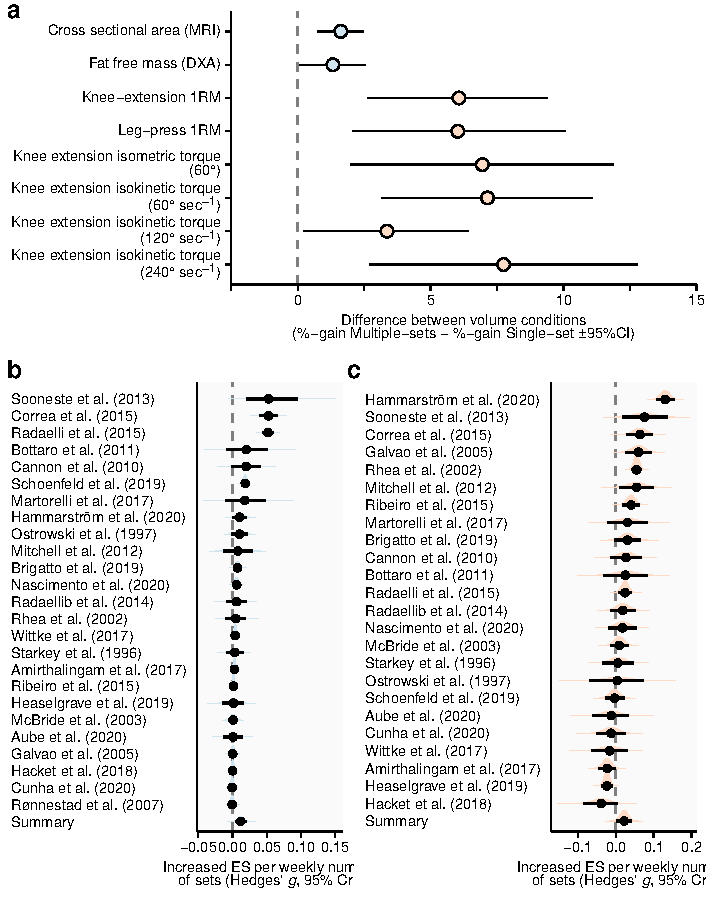
\includegraphics{thesis_files/figure-latex/comb-fig-s1-1} 

}

\caption[Differences in training induced changes to muscle mass and strength measures between volume conditions in Study I and weekly training volume meta-regression.]{Differences in training-induced relative changes in muscle-mass and strength (a). Estimates are derived from ANCOVA models controling for baseline values. Estimates from meta-regression models examining the effect of weekly number of sets per muscle group on muscle hypertrophy (b) and strength gains (c). Estimates are effect size measures (Hedges g) with 95\% credible intervals (CrI).}\label{fig:comb-fig-s1}
\end{figure}
\pagebreak

In an attempt to explain differences in training outcomes between volume-conditions, selected molecular markers, known to influence adaptations to resistance training were investigated for volume-dependency.
First, acute activation of signaling along the mechanosensitive mTORC1-pathway was measured in before and after the fifth training session in Study I.
A commonly used readout of mTORC1-signaling is the phosphorylation of S6-kinase (S6K1) at Thr\textsuperscript{389}/Thr\textsuperscript{412} which in turn precedes phosphorylation of ribosomal protein S6 (rpS6, see Figure \ref{fig:mtor-fig}a).
In the present study, exercise-induced S6K1\textsuperscript{Thr\textsuperscript{389}/Thr\textsuperscript{412}} phosphorylation was indeed shown to be volume dependent along with phosphorylation of rpS6\textsuperscript{Ser\textsuperscript{235/236}} and mTOR\textsuperscript{Ser\textsuperscript{2448}} (Figure \ref{fig:mtor-fig} b).
Together these observations indicates larger perturbations along the mTORC1 signaling axis which confirms previous studies showing exercise-volume dependency of mTORC1-related signaling in the acute phase (\textless{} 5 hours) after exercise, with the low-volume condition doing at least three sets activating the muscle under study
{[}250, 22, 21, 20,146{]}.
It is recognized that phosphorylation of mTOR itself at Ser\textsuperscript{2448} primarily should be regarded as indicative for negative feedback as this site is phosphorylated due to S6K1 activity
{[}295{]} (Figure \ref{fig:mtor-fig} a).
It is also recognized that the phosphorylation status of rpS6 at Ser\textsuperscript{235/236} is not solely due to mTORC1 signalling as both mTORC1 and extracellular signal-regulated kinases (ERK)-signalling converges here
{[}253{]}.
Interestingly, Terzis \emph{et al.} and Ahtiainen \emph{et al.} did not report any clear volume dependency in exercise-induced activation of ERK 1/2
{[}168, 22{]},
suggesting that any volume-dependent regulation of this pathway was outside the time-frame of these studies. However, it might also suggest that volume selectively modulates specific pathways in the acute phase after resistance exercise.
It should however be noted that the present, and previous studies are limited in their temporal resolution and different patterns over time in related to exercise-volume cannot be ruled out.

The importance of mTORC1 signalling for protein synthesis in the acute phase after resistance exercise is well established.
In humans, administration of rapamycin, a selective inhibitor of mTORC1, prior to resistance exercise leads to delayed or blunted activation of mTORC1 effectors such as
S6K1 and rpS6 as well as unchanged levels of phopshorylation of 4E-BP1 and eEF2 concomitantly with abolished exercise-induced increase in protein synthesis
{[}169{]}.
Volume dependent increase in mTORC1 signalling also coincide with larger protein synthesis rates
{[}20, 250{]}
As such, volume dependence of mTORC1-related signalling suggests that higher within-session volume can be regarded as leading to an increased potential for protein synthesis in the acute-phase after exercise.
Previous studies has indirectly linked mTORC1-related signaling to muscle growth as acute perturbation along this pathway has been correlated with muscle growth
{[}168, 296{]}.
However, this is not a consistent findings in the literature
{[}146, 297{]},
nor is it consistent with results in the present study as acute activation of S6K1 in response to the fifth session was not associated with training-induced changes in muscle mass.\footnote{Raw Spearman's correlations between exercise induced change in S6K1 phosphorylation and change in muscle mass (measured with MRI) indicated weak (insignificant) associations (\(\rho=\) -0.044 - 0.190) depedning on the isoform measured (p70 or p85) and number of sets. More elaborate modeling confirmed weak relationships between degree of phsophorylation and muscle mass change. When controlling for baseline values in degree of phsophorylation (as this influence the calculation of fold-change) and number of sets, standardized estimates for the effect of phosphorylation were (increase in \%-muscle mass change for every 1SD change in fold-change phsophorylation, with {[}95\% CI{]}) \(\beta=\) 0.33 {[}-0.53, 1.20{]} for p70 S6K1-p70\textsuperscript{Thr389} and \(\beta=\) 0.43 {[}-0.39, 1.25{]} for S6K1-p85\textsuperscript{Thr412}.}.
\begin{figure}

{\centering 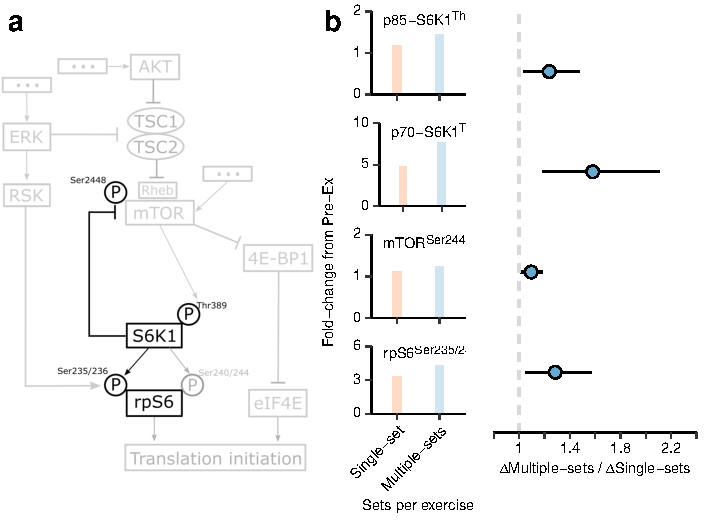
\includegraphics{thesis_files/figure-latex/mtor-fig-1} 

}

\caption[Differences between volume conditions in exercise induced phosphorylation of proteins related to mTORC1 signaling]{Measured phosphorylation sites in context (a) and differences between volume conditions in phosphorylation status of S6K1 at Thr \textsuperscript{389} (p70) Thr \textsuperscript{412} (p85), rpS6 at Ser \textsuperscript{235 236} and mTOR at Ser \textsuperscript{2448} induced by acute exercise and expressed as fold-changes (b). Estimates are derived from ANCOVA models controling for baseline values. Values in b are point estimates with 95\% confidence intervals.}\label{fig:mtor-fig}
\end{figure}
Although mTORC1 signaling most certainly contributes to protein synthesis in the acute recovery phase after resistance exercise {[}169{]},
its use as a predictor of training induced muscle hypertrophy is complicated by a number of reasons.
First, measuring its activity is not straight forward for biological reasons including pathway cross-talk and negative feedback as well as technical aspects
{[}192, 253, 298{]}.
Secondly, mTORC1 signaling is not a stable phenomenon either between or within individuals as short- and long-term resistance training leads to diminished activity along its pathway
{[}193, 194{]}.
Thirdly, mTORC1 readily integrate multiple signals but also convey these to multiple downstream processes
{[}189{]}.
As such, mTORC1 activity represent an early, transient response to resistance exercise with its signaling contributing to accumulative responses.
One such downstream target of mTORC1 is ribosomal biogenesis
{[}211, 197,\\
214, 187{]},
ultimately leading to accumulation of ribosomal RNA, a response typically seen in connection with to resistance training
{[}196,198, 193, 160{]}.

As ribosomal RNA is the most abundant constituent of muscle RNA it provides an estimate of muscle ribosomal abundance when expressed per unit tissue weight
{[}162, 164{]}.
From baseline to prior to the fifth training session (Week 2), total RNA per mg tissue increased by \(\sim\) 19 and 34\% in the single-set and multiple-sets condition, respectively. Total RNA levels were still elevated above baseline after the intervention (Week 12, single-set \(\sim\) 13; multiple-sets \(\sim\) 20\%). Similar patterns were seen in target analysis of ribosomal RNA using qPCR (single-set increase from baseline to Week 2 \(\sim\) 8-44\% and Week 12 \(\sim\) 14-36\%; multiple-sets \(\sim\) 31-57\% and Week 12 \(\sim\) 14-23\%). Comparing volume conditions revealed higher levels of total RNA and mature ribosomal RNA species in the multiple-sets condition at Week 2 (Figure \ref{fig:rrna-fig}a). At Week 12 differences between volume conditions were in total RNA less clear and ribosomal RNA 28S showing higher levels in the single-set leg (Figure \ref{fig:rrna-fig}a).
\begin{figure}

{\centering 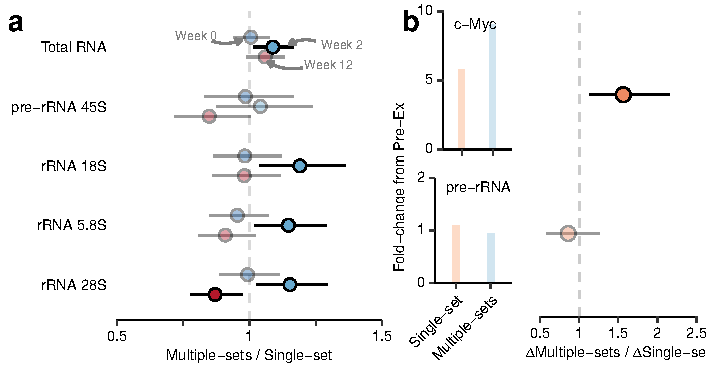
\includegraphics{thesis_files/figure-latex/rrna-fig-1} 

}

\caption[Differences between volume conditions total RNA and ribosomal RNA]{Differences between volume conditions in total RNA and ribosomal RNA-species (pre-rRNA 45S, rRNA 18S, rRNA 5.8S and rRNA 28S) measured at rest during the course of Study I (a). Acute changes in abundance of c-Myc mRNA and pre-rRNA 45S in response to acute exercise in Week 2 and differences between volume conditions (b). Errorbars represents 95\% confidence intervals, transparent points and errorbars signifies that the confidence interval contain 1.}\label{fig:rrna-fig}
\end{figure}
Analysis of c-Myc mRNA abundance in response to the fifth training session also showed volume-dependent regulation with exercise-induced increases being \(\sim\) 1.5-fold higher in response to the moderate- compared to the low-volume condition (Figure \ref{fig:rrna-fig}b). c-Myc represents a rapamycin-insesitive signaling pathway, paralell to mTORC1, known to also stimulating ribosomal biogenesis
{[}195, 216,299{]}.

Ribosomal biogenesis is an early adaptation to resistance training with initial increases in total RNA evident before any hypertrophy can be detected
{[}203, 205, 62, 63{]}.
The increase in ribosomal RNA represents an accumulation of ribosomes and an increased translational capacity. This improved translational capacity contributes to protein accreetion resulting in muscle hypertrophy, reflected in associations between measures of ribosome abundance (typically total RNA) and muscle hypertrophy
{[}198, 196, 199, 160{]}.
Due to the sequential nature of these events (increased translational capacity before muscle hypertrophy), early increases in total RNA would possible better reflect training-induced changes in muscle hypertrophy.
Any increase in muscle mass would also contribute to a dilution of the RNA pool
{[}280{]}
possibly masking their causal relationship.
Comparing the relationships between RNA abundance and muscle hypertrophy at different time-points supported this view as the amount of RNA at Week 2 showed the strongest relationship with the resulting muscle growth (Figure \ref{fig:rrna-csa-fig}, @table(rna-csa-tab)). This indicates that translational capacity, affected by exercise, early in the training program is determining training-induced changes in muscle mass.
\begin{table}

\caption{\label{tab:rna-csa-tab}Influence of RNA abundance on training-induced muscle growth measured with MRI}
\centering
\fontsize{8}{10}\selectfont
\begin{tabular}[t]{lrrrrll}
\toprule
\multicolumn{6}{c}{ } & \multicolumn{1}{c}{Standardized coefficients} \\
\cmidrule(l{3pt}r{3pt}){7-7}
 & Estimate & SE & df & \textit{t}-value & 95\% CI & Estimate [95\% CI]\\
\midrule
(Intercept) & -8.10 & 3.56 & 32 & -2.27 & [-15.35, -0.84] & \\
Moderate- vs. low-volume & 0.67 & 0.41 & 28 & 1.64 & [-0.17, 1.51] & \\
\addlinespace[0.3em]
\multicolumn{7}{l}{\textbf{RNA abundance (ng mg\textsuperscript{-1})}}\\
\hspace{1em}Week 0 & 0.00 & 0.01 & 28 & 0.37 & [-0.01, 0.02] & 0.12 [-0.54, 0.78]\\
\hspace{1em}Week 2 & 0.02 & 0.01 & 28 & 3.58 & [0.01, 0.03] & 1.40 [0.60, 2.21]\\
\hspace{1em}Week 12 & 0.01 & 0.01 & 28 & 1.43 & [-0.00, 0.02] & 0.57 [-0.25, 1.38]\\
\bottomrule
\multicolumn{7}{l}{\textsuperscript{a} Standardized coefficients scaled by its SD}\\
\end{tabular}
\end{table}
\begin{figure}

{\centering 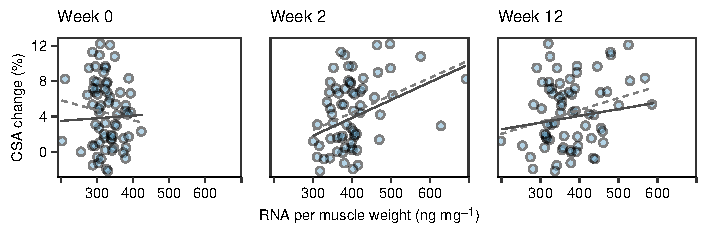
\includegraphics{thesis_files/figure-latex/rrna-csa-fig-1} 

}

\caption[Relationship between total RNA and training induced muscle growth]{Relationship between total RNA and training induced change in thigh cross sectional area (CSA) as measured by MRI. Dashed line represent naive relationship, solid line represent adjusted reliationship as seen in \\ref{table:rna-csa-tab}.}\label{fig:rrna-csa-fig}
\end{figure}
\hypertarget{volume-dependent-remodeling-of-muscle-fiber-type-composition}{%
\section{Volume-dependent remodeling of muscle fiber-type composition}\label{volume-dependent-remodeling-of-muscle-fiber-type-composition}}

Resistance training readily leads to remodeling of the muscle, this includes qualitative changes. These include fiber type transitions through changes in the myosin heavy-chain protein composition
{[}98, 99, 89, 101{]}.
Resistance-training induced changes in fiber-types identified by myosin heavy-chain expression occurs primarily as a IIX \(\rightarrow\) IIA transition which results in a more fatigue-resistant phenotype
{[}89, 100, 94{]}
and thus represent an important aspect of the adaptive response to resistance training by reversing effects of inactivity and disuse
{[}102, 103{]}.
In Study I, muscle fiber-type compositions were determined based on immunostaining of myosin heavy-chain protein in muscle cross-sections. The staining protocol allowed for the identification of Type I (red), Type IIA (brown), Type IIX (unstained), and Type IIA/IIX hybrids (light brown, Figure \ref{fig:myhc-fig}a). Throughout the study, a general reduction in Type IIX fibers was seen as pure Type IIX was replaced with Type IIA/IIX hybrids at Week 2, and these, in turn, were measured at lower proportions at Week 12 (Figure \ref{fig:myhc-fig}b).

When comparing volume conditions, moderate training volume led to more pronounced down regulation of the \emph{MYH1} gene, coding for Type IIX myosin heavy-chain protein, at all time-points during the intervention (Figure \ref{fig:myhc-fig}c). This presumably led to the accumalative effect seen after twelve weeks of training where the proportion of Type IIX fibers was lower in the moderate- compared to the low-volume condition (indicative as an odd-ratio (OR) \textless{} 1, OR {[}95\% CI{]}: 0.54 {[}0.31, 0.94{]}, combined measure of IIX/IIA hybrids and pure IIX fibers, Figure \ref{fig:myhc-fig}d).\\
This underlines that training volume is an important factor for fiber-type composition remodeling. Although not surprising, similar observations are lacking in the litterateur as previous studies have not compared this transition directly between volume protocols.
However, when comparing non-exhaustive high-load resistance training to load-matched training to volatile failure, Pareja-Blanco \emph{et al.} observed a blunted IIX \(\rightarrow\) IIA transitions in response to the non-exhaustive protocol
{[}300{]}.
Together these data indicates that increased metabolic stress and/or dosage of neuromuscular activity are plausible candidates for regulation of IIX \(\rightarrow\) IIA reprogramming in humans in response to resistance training.
This as opposed to a tensile stimuli.
Based on observations in animal models, neural input might however be considered the primary candidate.
For example, in a rat model of resistance training, force did not affect fast-to-slow fiber-type transitions when performed with the same electrical stimulation pattern, indicating that neural activity governs fiber-type transitions
{[}223{]}.

At Week 2, a more pronounced reduction in \emph{MYH1} gene abundance in the moderat-volume condition did not translate to the protein level. Instead a greater number of fibers were classified as IIX in the moderate-volume condition compared to the low-volume condition (OR: 1.56 {[}1.06, 2.32{]}).
The moderate-volume condition thus showed an even greater mismatch between gene and protein levels.
Such mismatch is seen after resistance-exercise and is indicative for early transition of muscle fibers
{[}100{]}.
Interestingly, the difference between volume conditions was driven by less Type IIX expression in the low-volume condition.
This indicates that remodeling occurred faster in response to the low-volume condition despite a greater ``transition signal'' in the moderate-volume leg.
A plausible explanation to this observation could be that the greater damage caused by a greater training stimuli lead to a delayed fiber-type transition.
This hypothesis is supported by observations indicating that a proportion of the protein synthesis seen early in a resistance-training period can be attributed to tissue repair rather than myofibrilar synthesis
{[}153, 301{]}.
Regardless of causality, the more rapid early adaptation seen in response to a lower training volume suggests that optimized resistance training should include a progressive volume component.

\pagebreak
\begin{figure}

{\centering 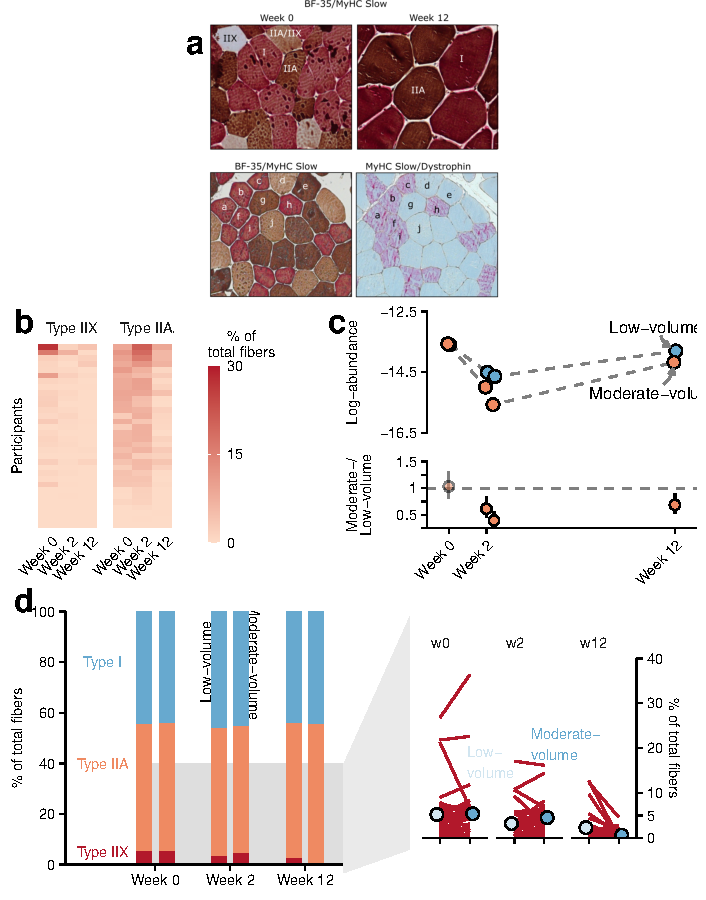
\includegraphics{thesis_files/figure-latex/myhc-fig-1} 

}

\caption[Fiber-type composition in Study I]{Representative muscle cross-sections stained for myosin-heavy chain isoforms are shown in (a). Using antibodies for Type I (MyHC Slow) and all but Type IIX (BF-35) enabeled separating Type I fibres from other fibres (red stain, a lower panel). Type IIX fibers were indentified as unstained, and weak brown staining was analysed as Type IIX/IIA hybrids (a, upper panel). Resistance training led to a reduction in Type IIX and IIX/IIA hybrids, (b) shows participant-average Type IIX and IIX/IIA percentages. Training led to reduction in \textit{MYH1} gene expression, and more so in the moderate-volume condition, evident from pairwise comparisons in (fold-differences with 95\% CI, c). Differeces in protein expression of Type IIX fiber (counted as pure IIX + 0.5 $\times$ IIX/IIA hybrids) reversed throught the study as the moderate-volume condition showed greater proprtions of IIX fibers at Week 2 but lesser expression at Week 12 (d).}\label{fig:myhc-fig}
\end{figure}
\pagebreak

\hypertarget{volume-dependent-effects-on-transcriptome-characteristics}{%
\section{Volume-dependent effects on transcriptome characteristics}\label{volume-dependent-effects-on-transcriptome-characteristics}}

As already \protect\hyperlink{muscle-mass-growth}{discussed}, resistance training in Study I led to an increase in total RNA per unit tissue weight. Furthermore, the magnitude of this increase was different between volume conditions (see Figure \ref{fig:rrna-fig}).
Studies of gene expression, using techniques such as qPCR or RNA sequencing, comes with the assumption that an equal amount of biological material is used when evaluating abundance of a single transcript.
It is therefore common that a normalized amount of total RNA is used in sample preparation to satisfy such an assumption
{[}119, 240, 302{]}.
However, if the ratio of RNA to tissue mass has changed throughout a study, analyses are performed on a different amount of tissue. This may be the case after a resistance-training intervention, or between study conditions, as in Study I.
Indeed, by calculating the amount of tissue used when preparing samples for RNA sequencing it is obvious that the increased amount of total RNA per-unit-muscle weight results in a situation where samples are prepared from a lesser amount of tissue.
This effect was more pronounced in response to the moderate- compared to the low-volume condition (Figure \ref{fig:lib-size-fig}a).
Total library sizes were quantified from RNA sequencing as the total number of quantified gene counts, this revealed a general increase in library sizes in response to resistance training, however, the increase was more apparent in the low-volume condition
(Figure \ref{fig:lib-size-fig}b).
When library sizes were normalized to the amount of tissue used in sample preparation, differences between conditions were diminished
(Figure \ref{fig:lib-size-fig}c).
This suggests that resistance-training leads to an increased global mRNA expression per-unit-muscle weight (43-53\% in the present study). However, this increase was not different between volume-conditions, suggesting that a volume-dependent regulation of global RNA transcription primarily relates to transcription of RNA-fractions other than mRNA (likely rRNA, see Figure \ref{fig:rrna-fig}).
\begin{figure}

{\centering 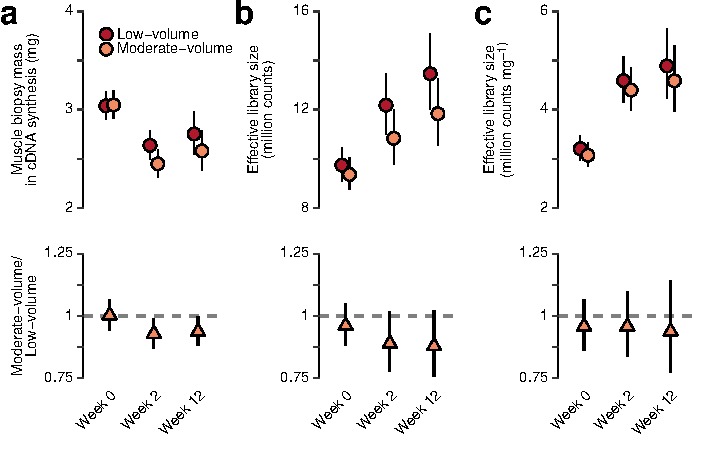
\includegraphics{thesis_files/figure-latex/lib-size-fig-1} 

}

\caption[Muscle weight and RNA-seq library size]{Less muscle tissue was used for cDNA synthesis in the moderat- compared to low-volume condition as a result of total RNA increases per tissue weight (a). Library sizes tended to be greater in the low-volume condition (b), after normalizing library sizes to muscle weight differences were diminished (c). Lower panels shows differences between volume conditions}\label{fig:lib-size-fig}
\end{figure}
Although the observed increase in library sizes suggested a global increase in mRNA transcription, it did not resemble global gene amplification seen in models with experimentally manipulated c-Myc protein expression
{[}246, 244{]}.
Instead, the majority of identified genes were categorized as having unchanged levels per amount of tissue from baseline to Week 2 (73.3\%) and Week 12 (88.4\%). A small fraction of genes were identified as being less abundant (Week 2, 0.51\%; Week 12, 0.01\%) and the remaining genes were identified as more abundant at Week 2 (26.2\%) and 12 (11.6\%), respectively.
Gene-set enrichment analyses revealed that training-induced changes in gene expression profiles were related to increased abundance of genes related to extracellular matrix remodeling, collagen synthesis and inflammatory processes. Although these observations were made without a proper control to investigate training-induced effects \emph{per se}, they resembles previous (controlled and uncontrolled) studies characterizing skeletal muscle tissue in response to heavy mechanical loading, in the acute phase
{[}303, 304, 118, 121{]},
and after prolonged training {[}120, 119{]}.
\begin{figure}

{\centering 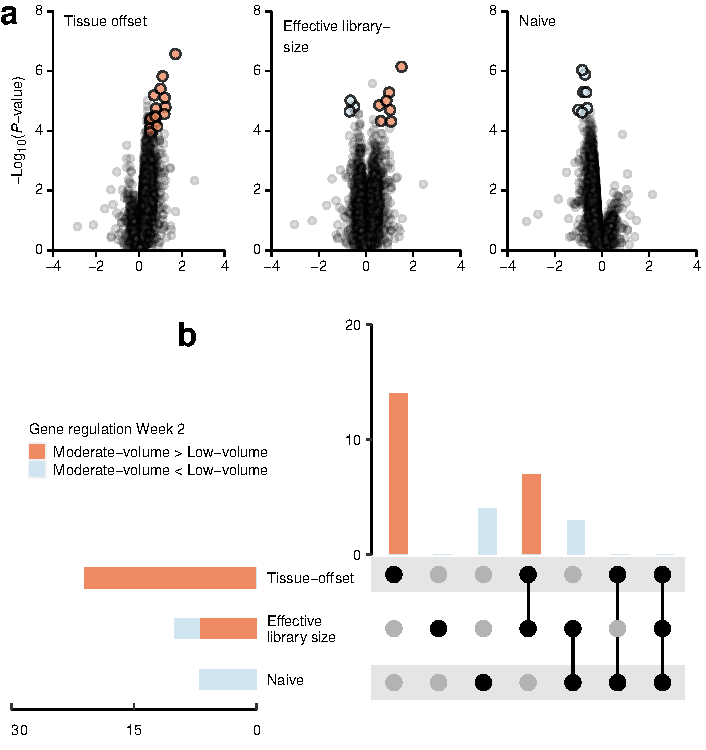
\includegraphics{thesis_files/figure-latex/week2-upset-volcano-1} 

}

\caption[General patterns of differentially expressed genes at Week 2]{Volume dependent differences in gene expression in different models (a) either accounting for the amount of tissue used in cDNA synthesis (Tissue offset), library sizes or un-normalized (Naive). Genes identified as differentially expressed (log2 fold-change > |0.5|, FDR < 0.05) are highlighted in a.  Overlap in differentially expressed genes between models are shown in (b)}\label{fig:week2-upset-volcano}
\end{figure}
As we observed volume-dependent differences in the ratio of total RNA to tissue weight, leading to differences in biological input in sample preparation, we used three different normalization strategies to characterize volume-dependence in transcriptome characteristics.
By implementing each normalization strategy as variations of generalized linear mixed models (GLMM), we could compare outcomes related to conceptually different normalization techniques using the same statistical framework.
The use of GLMM also had the benefit of accounting for the study design which included correlated data (within participants)
{[}279{]}.
The model with most parameters included an offset term expressing gene counts per tissue weight. This was combined with library size included as a fixed effect in the model together with study conditions, time and volume-conditions (tissue offset-model).
In a second model, the offset term was removed, thus only the library size was used to normalize the gene counts, as suggested by Cui \emph{et al.}
{[}279{]} (effective library-size model).
For comparison, a naive model containing no normalization-parameters was also included in analyses.
At Week 2, tissue-offset normalization (modeling mRNA counts per-mg-muscle weight) revealed a general shift of mRNA counts towards the moderate-volume condition (Figure \ref{fig:week2-upset-volcano}a).
This was in contrast to patterns found when using library-size and naive models resulting in a pattern where the ``conventional'' normalization strategy, accounting only for library sizes more resembled the non-normalized naive model as there was an overlap of genes identified as differentially expressed between the models (Figure \ref{fig:week2-upset-volcano}b).
Gene-set enrichment analyzes revealed that genes related to extracellular matrix remodeling and collagen synthesis was driving the difference in transcriptome profiles between volume-conditions at Week 2
(Figure \ref{fig:week2-go-analysis}a).
This was apparent using both the tissue offset model and the library-size normalized model, however volume-dependent effects were more pronounced in the tissue-offset model
(Figure \ref{fig:week2-go-analysis}b).
\begin{figure}

{\centering 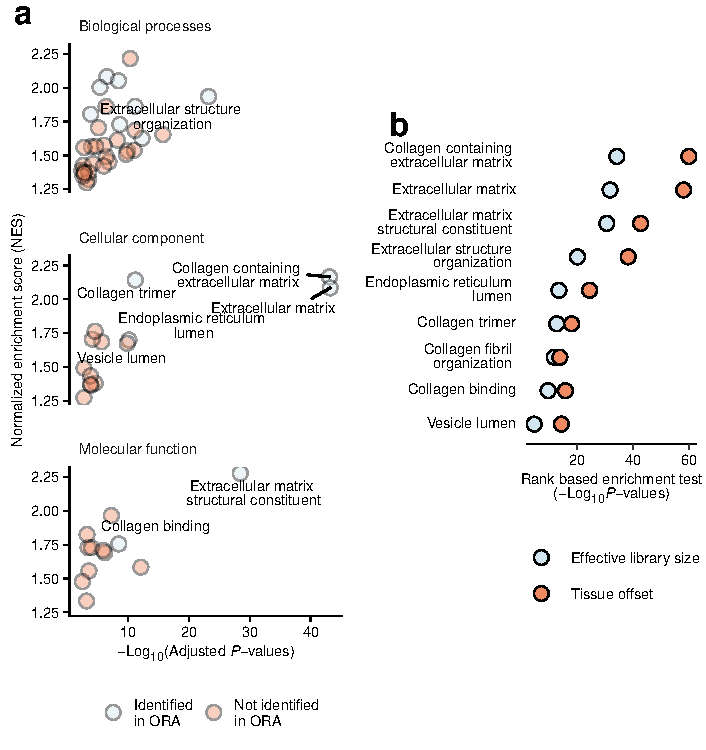
\includegraphics{thesis_files/figure-latex/week2-go-analysis-1} 

}

\caption[Gene-set enrichment analysis at Week 2]{Gene-set enrichment analysis based on gene-ontology gene sets and estimates from the tissue-offset model (a). Adjusted \textit{P}-values and Normalized enrichment scores are retrieved from analysis of directional rank-based tests (GSEA), labeling of points indicate if gene-sets were also identified from differentially expressed genes (Log2 fold-change >|0.5|, FDR < 0.05). In (b) comparison between the tissue-offset and library size normalization models are shown in rank-based (non-directional, cerno-test) analysis of gene ontology gene sets.}\label{fig:week2-go-analysis}
\end{figure}
Differences in normalization models led to global shifts of estimates of differences between volume conditions. Figure \ref{fig:gene-set-rug} shows this global shift as density curves representing all fold-changes between volume conditions. Accounting for the amount of muscle mass in sample preparations shifted also specific gene-sets towards greater differences between volume conditions, this is exemplified in Figure \ref{fig:gene-set-rug} by the gene set ``Collagen containing extracellular matrix.''
\begin{figure}

{\centering 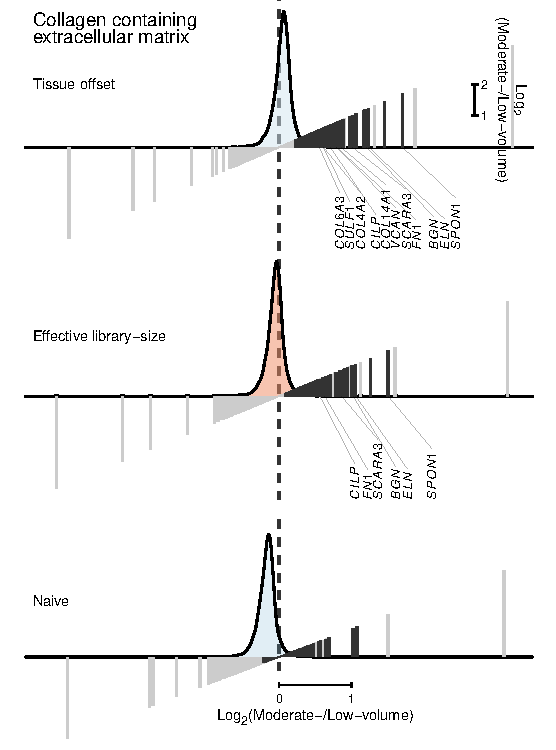
\includegraphics{thesis_files/figure-latex/gene-set-rug-1} 

}

\caption[Global shifts in volume-dependent fold change as an effect of normalization methods at Week 2]{Differences between volume conditions at Week 2 as seen using different normalization models. Shifts in the full distribution of Log2-fold change values between volume conditions were seen between on normalization models (density curves). As an example, genes associated with the \textit{Collagen containing extracellular matrix} gene set are highlighted (black bars), differentially expressed genes are identified with gene symbols in each method.}\label{fig:gene-set-rug}
\end{figure}
At week 12, differences seen at Week 2 between volume conditions derived from the tissue-offset model were abolished (Figure \ref{week12-upset-volcano}a). Volume dependent differences were seen in the library-size normalized model, however, these overlapped with the naive model indicating that imbalance in muscle tissue between conditions may have contributed to global shifts in favor of the low-volume condition. This indicates that after initial perturbations related to different training volumes, the muscle may have reached a new transcriptional equilibrium.
\begin{figure}

{\centering 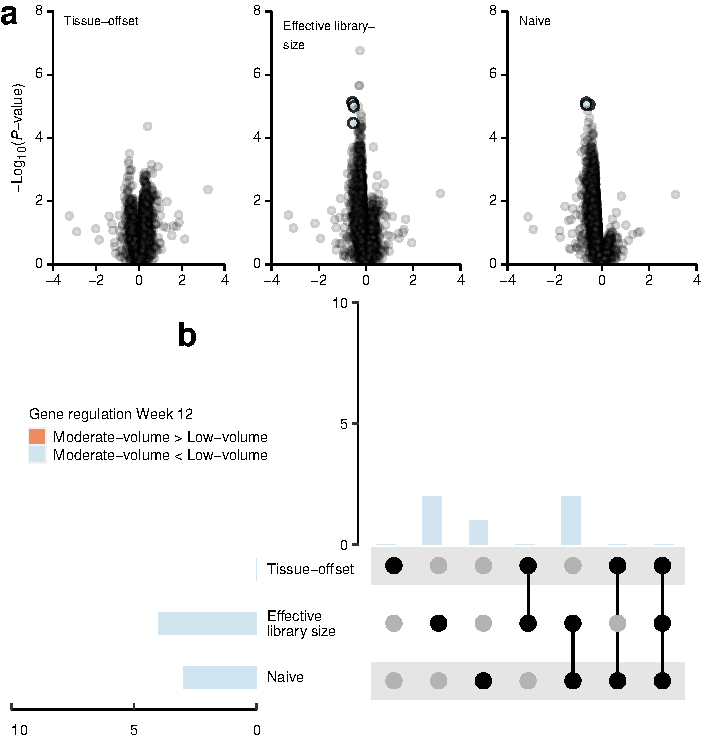
\includegraphics{thesis_files/figure-latex/week12-upset-volcano-1} 

}

\caption[General patterns of differentially expressed genes at Week 12]{Volume dependent differences in gene expression in different models (a) either accounting for the amount of tissue used in cDNA synthesis (Tissue offset), library sizes or un-normalized (Naive). Overlap in differentially expressed genes between models are shown in (b)}\label{fig:week12-upset-volcano}
\end{figure}
From a general perspective, this analysis underlines the importance of a well considered choice of normalization strategy in studies of gene expression in non-homeostatic conditions
{[}305, 248, 244{]}.
Specifically, in gene expression studies of training-induced muscle hypertrophy, an ill-advised normalization strategy could mask or overestimate differences between experimental conditions as different amount of tissue is being used in sample preparation. This as a consequence of a normalized RNA input between different conditions. Differences in tissue used in sample preparation between volume-conditions in Study I effectively led to an underestimation of genes identified as differentially expressed at Week 2 and led to nonsensible identification of differentially expressed genes at Week 12.
The choice of normalization strategy ultimately determines the definition of differential expression. By using the tissue offset model we were interested in gene counts per tissue, as opposed to using the the library size as the denominator in analyses, leading to gene counts expressed per transcriptome. Although both strategies may have merit in certain situations, selected genes may be better studied as counts per amount of tissue. It could be argued that one such group of genes are genes related to extracellular matrix remodeling.
First, extracellular matrix-related genes have been shown to display close association between mRNAs abundances and their respective proteins, including collagen-organization proteins {[}306{]}..
This indicates that remodeling on the protein level to a large degree is determined transcriptionally.
Secondly, selected extracellular-matrix related genes are not expressed in muscle fibers but instead in neighboring cells (e.g.~fibroblasts)
{[}307, 116{]}.
Thus assuming that an increase in total RNA due to increased ribosomal biogenesis would scale to other cell types in muscle tissue might affect the interpretation of such gene expression data.
Consequently, studies of transcriptional regulation of extracellular matrix remodeling in relation to muscle hypertrophy should account for the amount of tissue used in analyses.

Previous studies have generally not found extracellular matrix remodeling to be affected by different exercise variables. Instead, when comparing low- and high-load, Holm \emph{et al.} found similar responses measured as collagen synthesis {[}118{]}..
Similarly, eccentric versus concentric resistance exercise did not affect muscle collagen synthesis differently
{[}121{]}.
Although it should be noted that the measurement of collagen synthesis and expression of genes related to extracellular matrix are targeting different aspects of extracellular matrix remodeling. Volume-dependent regulation of these target genes, implicates this remodeling as paralleled with muscle growth.

In response to acute exercise, 4.7 and 6.9\% of identified genes were categorized as up and down-regulated 1 hour after exercise.
These changes were measured as per transcriptome as no changes in the total RNA per tissue weight
{[}280{]},
but instead fluid shifts {[}281{]}
could be expected in the short time frame affecting the estimate of muscle weight from wet tissue.
Differentially regulated genes were generally associated with stress responses including inflammation and immune responses as well as extracellular matrix related processes. In contrasts to long term changes, acute exercise led to down-regulation of extracellular matrix-related genes, similarly to what have been found by others {[}120{]}.
Regarding volume-dependent regulation in the acute phase, only a single gene was found to be differentially expressed between volume-conditions. This gene, \emph{RFT1}, which was found to be down-regulated and more so in response to moderate-volume exercise is associated lipid transport, carbohydrate transport, and endoplasmic reticulum membrane and has previously been found to be decreased in muscle after exercise {[}308{]}.
Further analyses of volume-dependent differences not relying solely on arbitrarily defined differential expression confirmed that no strong differences were evident in transcriptome characteristics in this short time-span.
It is likely that the timing of the post-exercise biopsy missed more relevant volume-dependent regulation in the acute phase.

\hypertarget{determinants-of-moderate--over-low-volume-training-benefit}{%
\section{Determinants of moderate- over low-volume training benefit}\label{determinants-of-moderate--over-low-volume-training-benefit}}

To explore determining factors for additional benefit of moderate-volume training, individual differences in muscle-hypertrophy (CSA) and average muscle strength between the moderate- and low-volume condition were calculated. In primary analyses, difference-scores were dichotomized to \emph{additional benefit of moderate-volume training} or \emph{no additional benefit of moderate-volume training} based on the smallest worthwhile change (SWC) in the direction of moderate-volume. Participants were thus identified as having \emph{additional benefit of moderate-volume training} if the difference in raw change scores were greater than the between-participants baseline SD \(\times\) 0.2 in favor of moderate-volume training.\footnote{Sex-differences were accounted for by mean-centering variables prior to SD estimation. A weighted SWC was calculated for the strength variable to avoid underestimating SD.}
The choice of using a dichotomized response variable (benefit vs.~no benefit) was made to maintain an individual perspective; irrespective of the magnitude of the individual difference, what determines benefit of moderate- over low-volume training?
\begin{figure}

{\centering 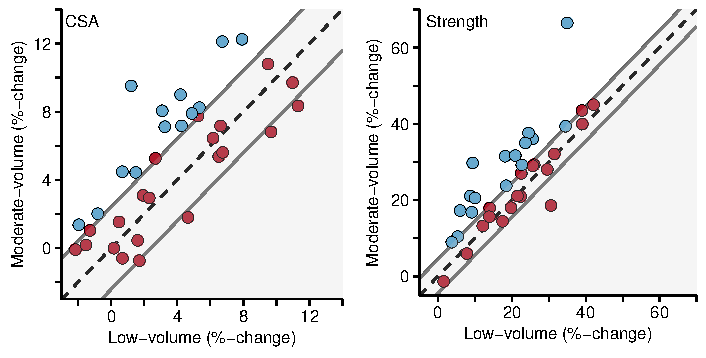
\includegraphics{thesis_files/figure-latex/csa-str-sets-corr-1} 

}

\caption[]{Relationship between individual responses to moderate- and low-volume training. Dashed lines are identity lines ($y = x$) and the distance from identity lines to solid lines represent the smallest worthwhile change (SWC) in each variable.}\label{fig:csa-str-sets-corr}
\end{figure}
Identification of participants as belonging to the benefit- or no benefit-group, respectively, for each outcome variable is visualized in Figure \ref{fig:csa-str-sets-corr}. Responses to either training condition were highly correlated for both muscle CSA (\emph{r} = 0.750, {[}0.552, 0.868{]}) and average strength (\emph{r} = 0.805, {[}0.552, 0.868{]}), but participants identified as having benefit of moderate-volume training were identified across the whole range of responses (Figure \ref{fig:csa-str-sets-corr}).

With the aim to develop parsimonious models that explained benefits of moderate-volume training in each outcome (muscle CSA and average strength), a set of potential determinants was selected prior to any association analysis. These included blood variables, baseline strength and muscle mass, volume-dependent molecular responses to training and baseline fiber-type composition. Additionally, pre-study training habits and training characteristics during the study as well as dietary data were used in an initial screening process of potential variables. As neither pre-study training habits (strength or other type physical training), within-study training characteristics (number of sessions completed and supervised) or dietary data displayed any differences between benefit-classifications, they were excluded from further consideration. So were also a set of continuous variables that did not meet the criteria for inclusion, based on preliminary univariate analysis\\
{[}288{]}.
Figure \ref{fig:univariate-benefit-analysis} shows continuous variables used in the initial screening process. Variables were kept for further consideration when the mean difference 80\% CI (thick error bars) did not containing the null-hypothesis of no difference between benefit-classification groups. Based on the variables selected in this first step, 32 participants were included in the subsequent analysis as two participants had missing values in one or more of the selected predictors.
\begin{figure}

{\centering 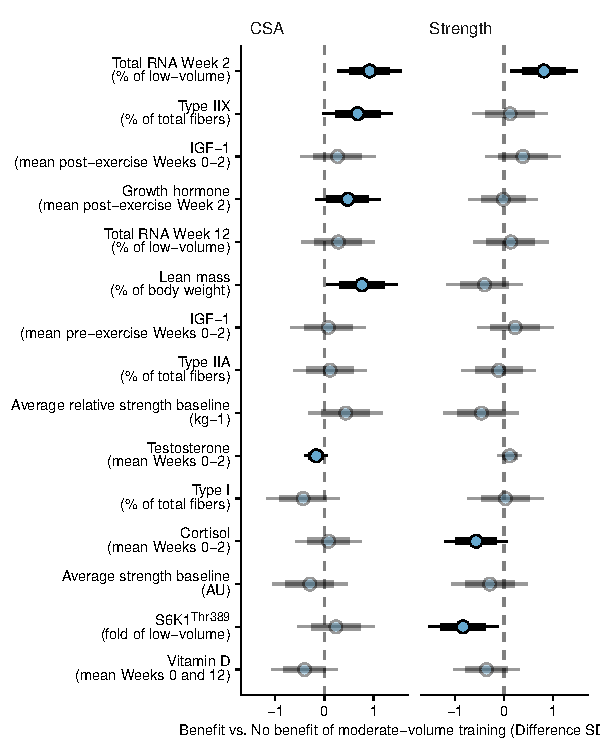
\includegraphics{thesis_files/figure-latex/univariate-benefit-analysis-1} 

}

\caption[Univariate analysis of potential determinants of benefit to moderat- over low-volume training]{Differences between groups classified as either having benefit or no benefit of moderate-volume training. For the sake of comparison, all variables have been scaled by their SD. Thick errorbars indicate a 80\% CI and thin errorbars indicate the 95\% CI. Transparent points and errorbars indicate that the variables was removed from further modeling. Sex was included as a covariate in all comparisons.}\label{fig:univariate-benefit-analysis}
\end{figure}
The choice of a dichotomized response variable (benefit vs.~no benefit) entailed the use of logistic regression. An assumption of this type of regression modeling is linearity of the logit
{[}288{]}.
As all variables did not meet this assumption when fitted in logistic regression they were categorized into biologically meaningful categories (Vitamin D insufficient/sufficient), dichotomized based on measurement detection limits (testosterone in females) or sex-specific median values (lean body mass and testosterone in males).
A stepwise approach was used to remove variables that did not display association with the response variables. Figure \ref{fig:model-reduction-plot} shows the process of stepwise removal of predictors.
Additional benefit of moderate- over low-volume training on muscle CSA was predicted by individual differences between volume conditions in Total RNA at Week 2 and baseline lean body mass dichotomized to above or below the sex-specific median.
For muscle strength, only individual differences between volume conditions in Total RNA at Week 2 remained in the model after variable selection.
\begin{figure}

{\centering 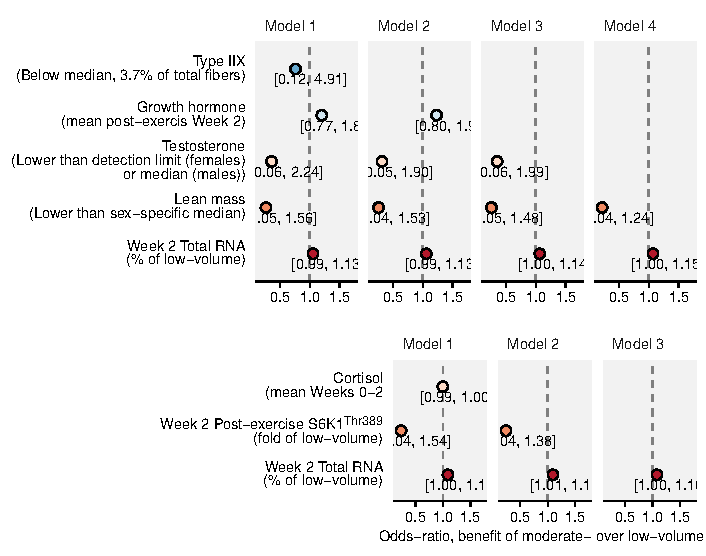
\includegraphics{thesis_files/figure-latex/model-reduction-plot-1} 

}

\caption[Step-wise variable selection of determinants of moderate- over low-volume training benefit.]{Sequential removal of predictors of moderate-volume benefit. Point estimates for each predictor are displayed with 95\% confidence intervals.}\label{fig:model-reduction-plot}
\end{figure}
The rationale for using dichotomized outcomes was, as mentioned above, to specifically explore determinants of \emph{individual} benefit of additional training volume, regardless of the magnitude of the difference between conditions.
This choice of analytic approach arose from discussions regarding clinical decision-making, where the potential benefit in each individual should guide the choice of training methods.
Although linked to the specific study question, a dichotomized outcome variable could potentially mask other important associations in the data due to loss of information associated with the transformation
{[}309{]}.
A primary hypothesis in the study was that the baseline muscle phenotype, specifically a ``glycolytic'' vs.~a ``aerobic'' phenotype (measured as high vs.~low type IIX content) would not show relative benefit of moderate-volume training.\footnote{\href{https://clinicaltrials.gov/ct2/show/NCT02179307?term=lillehammer\&draw=2\&rank=9}{As outlined in the Study's pre-registration}}
If such a marker would hold any prognostic value, it could potentially guide decisions regarding the training process.
In analysis, the phenotype marker measured as Type IIX counts was included together with other potential predictors of individual benefit of higher training-volume.
Both pre-training characteristics that could aid in clinical decision making and markers arising from the training itself were included in the analysis.
In order to select important determinants from this set of potential determinants, a stepwise procedure for variable selection, known as purposeful selection was used
{[}288{]}.
Generally, stepwise variable selection has been criticized for a number of reasons, including arbitrarily searching for a single best model, over-estimation of regression parameters and sensitivity to small changes in the investigated data set
{[}310, 309{]}.
In order to address the above mentioned limitations, the question was slightly rephrased in a secondary analysis presented here to explore the association between potential determinants and individual differences between moderate- and low-volume training.
As shown in Figure \ref{fig:continuous-determinants}a, only Total RNA content at Week 2 in the moderate-volume leg, expressed as a percentage of the low-volume leg RNA content, positively associated with differences between volume conditions in muscle hypertrophy (CSA) and strength gains. These relationships are plotted in Figure \ref{fig:continuous-determinants}b.

Together with previous studies
{[}196, 198, 199{]},
as well as the direct correlation between RNA content and muscle hypertrophy presented earlier in this text
(Figure \ref{fig:rna-csa-fig}),
this underlines the importance of early-phase ribosomal accumulation as a determining factor for training-induced muscle hypertrophy.
Participants showing greater increases in ribosomal content in response to higher training volume also displayed greater relative benefit of the higher volume.
This likely acts through an increased translational capacity and confirms observations regarding volume-dependence in regulation of total RNA, mature rRNA species (rRNA 18S, 28S and 5.8S) and subsequent muscle hypertrophy (and strength gains).
\begin{figure}

{\centering 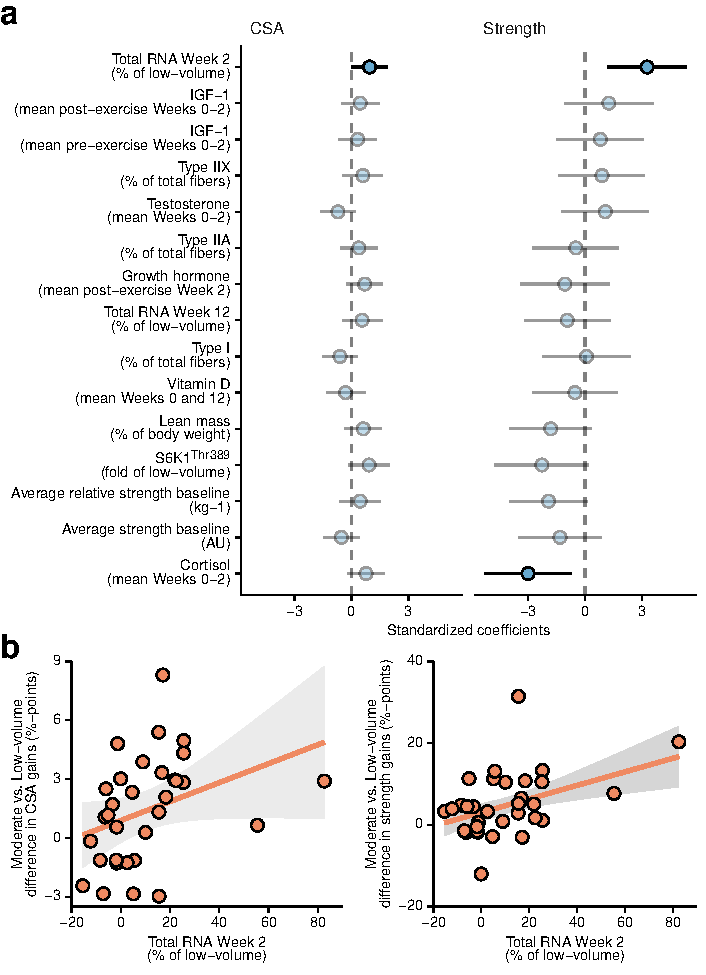
\includegraphics{thesis_files/figure-latex/continuous-determinants-1} 

}

\caption[Predictors of differences in outcomes between moderate- and low-volume training. Values in (a) are standardized regression coefficients with 95\% CI from univariate robust regression. Positive estimates indicate a positive association. Variables related to blood parameters, body composition and muscle strength was mean centered per sex.]{Analysis of association between potential predictors and individual differences between moderate- and low-volume training in muscle cross-sectional area and muscle strength as the dependent variable (a).}\label{fig:continuous-determinants}
\end{figure}
In primary analyses, percentage of lean body-mass was identified as a predictor of additional benefit of moderate-volume training on on muscle hypertrophy.
Albeit associated with a large degree of uncertainty, this indication was in line with current prescription guidelines recommending greater training volume for experienced individuals
{[}17{]}.
When analyzed between benefit categories, participants that displayed benefit of moderate- over low-volume training had a 4.3\%-point {[}0.3, 8.3{]} higher lean body mass compared to participants in the no benefit-group.
Lean body mass did not, however, display a linear relationship with individual differences between volume-conditions.
This together with the fact that we did not find any robust relationship between pre-training Type IIX fiber proportions and differences in training outcomes between volume conditions underlines that such markers have low prognostic value, even though they are readily adapted to the training regime as such.
This likely relates to the fact that traits such as fiber type, or body composition are genetically determined
{[}311, 95{]}
in addition to influenced by any history of physical activity.

\hypertarget{predictors-of-additional-benefit-of-added-training-volume-meta-analysis}{%
\subsection{Predictors of additional benefit of added training volume: Meta-analysis}\label{predictors-of-additional-benefit-of-added-training-volume-meta-analysis}}

To further explore potential factors associated with benefit of added training volume, interactions between study parameters and weekly number of sets were estimated from meta-regression models (previously reported without interactions in Figure \ref{fig:comb-fig-s1}).

Weekly number of sets did not interact with age, training status or sex for either muscle mass or strength (interaction estimates are shown in Table \ref{tab:meta-interaction-table}), indicating that the literature currently gives little support for such demographic variables to guide prescription regarding training volume.

In contrast to what has been previously reported
{[}25{]},
the present analysis did not indicate any robust differences between unspecific (e.g.~DXA) or specific (e.g.~MRI or muscle thickness measured with ultrasound) measures of muscle mass.
However, specific assessment of muscle strength, e.g.~measures of one repetition maximum in exercises used in the training program consistently showed larger positive effects of additional volume (Table \ref{tab:meta-interaction-table}).
Unspecific assessments of muscle strength were shown not to reflect additional training volume (effect size change per one weekly additional set 95\% CrI: {[}-0.027, 0.025{]}). This may indicate that specific motor learning is a factor influenced by training volume.

A consistent finding between measures of muscle mass and strength was the negative effect seen in upper- compared to the lower-body measures.
These results suggests that adding a weekly set to upper-body programs will not robustly lead to an increased effect in strength measures (upper-body effect size change for every additional weekly set 0.003 {[}-0.014, 0.02{]}).
The effect of an additional weekly set in the upper-body for measures of muscle mass was still positive (0.011 {[}0.002, 0.021{]}) albeit lower when compared to the effect seen in the lower body (Table \ref{tab:meta-interaction-table}).
Together this indicate that muscles more active in every day activities will benefit to a greater extent by additional training volume, compared to upper-body muscles.
Studies examining volume-dependence in molecular determinants to resistance-training adaptations between different muscle groups are limited.
However, Hanssen \emph{et al.} found different satellite cell activation between volume-conditions in \emph{m. vastus lateralis} but not in \emph{m. trapezius}, coinciding with volume-dependence in outcomes in lower- but not upper-body muscles
{[}145,256{]}.
Whether satellite cells \emph{per se} were responsible for this effect or if it represents a general inability of upper-body muscles to differentiate between two relatively strong stimuli remains to be explored.

The length of study interacted differently in muscle mass and strength models were longer training periods seemed to reduce the positive effect of added training volume on muscle mass, albeit likely to negligible degree. However strength outcomes were positively influenced by the length of the training period (Table \ref{tab:meta-interaction-table}). This may be an effect of different time courses in muscle mass and strength measures in response to resistance training.
\begin{table}

\caption{\label{tab:meta-interaction-table}Interaction between study parameter and weekly number of sets from meta-analyses on muscle mass and strength}
\centering
\fontsize{7}{9}\selectfont
\begin{tabular}[t]{lllll}
\toprule
\multicolumn{1}{c}{ } & \multicolumn{2}{c}{Muscle mass} & \multicolumn{2}{c}{Muscle strength} \\
\cmidrule(l{3pt}r{3pt}){2-3} \cmidrule(l{3pt}r{3pt}){4-5}
Interacting variable & Estimate & 95\% CrI & Estimate & 95\% CrI\\
\midrule
\addlinespace[0.3em]
\multicolumn{5}{l}{\textbf{Age}}\\
\hspace{1em}30-50 vs. 18-20 years & -0.011 & [-0.044, 0.02] & -0.037 & [-0.103, 0.028]\\
\hspace{1em}50- vs. 18-20 years & -0.004 & [-0.025, 0.016] & 0.005 & [-0.034, 0.044]\\
\hspace{1em}Mixed ages vs. 18-20 years & 0.005 & [-0.047, 0.055] & 0.005 & [-0.083, 0.092]\\
\addlinespace[0.3em]
\multicolumn{5}{l}{\textbf{Training status}}\\
\hspace{1em}Trained (> 1 year RT) vs. untrained & -0.001 & [-0.019, 0.016] & -0.025 & [-0.058, 0.007]\\
\addlinespace[0.3em]
\multicolumn{5}{l}{\textbf{Sex}}\\
\hspace{1em}Female vs. male & 0.001 & [-0.014, 0.015] & -0.012 & [-0.045, 0.018]\\
\hspace{1em}Mixed sex vs. male & -0.013 & [-0.038, 0.012] & 0.009 & [-0.044, 0.059]\\
\addlinespace[0.3em]
\multicolumn{5}{l}{\textbf{Body portion}}\\
\hspace{1em}Upper-body vs. lower-body & -0.005 & [-0.008, -0.002] & -0.029 & [-0.038, -0.02]\\
\hspace{1em}Whole-body vs. lower-body & -0.012 & [-0.034, 0.01] &  & \\
\addlinespace[0.3em]
\multicolumn{5}{l}{\textbf{Measurement technique}}\\
\hspace{1em}Unspecific vs. Specific estimation & -0.004 & [-0.01, 0.003] & -0.031 & [-0.06, -0.005]\\
\addlinespace[0.3em]
\multicolumn{5}{l}{\textbf{Length of study}}\\
\hspace{1em}Weeks & -0.001 & [-0.001, 0] & 0.005 & [0.003, 0.006]\\
\bottomrule
\end{tabular}
\end{table}
\hypertarget{characteristics-of-early-phase-training-induced-ribosome-biogenesis}{%
\section{Characteristics of early-phase training-induced ribosome biogenesis}\label{characteristics-of-early-phase-training-induced-ribosome-biogenesis}}

Total RNA seems to be a valid proxy marker of ribosomal density, as most of the RNA is assumed to be ribosomal RNA
{[}163{]},
which in turn is a valid marker of translational capacity
{[}164{]}.
Several studies have shown that total RNA content is altered by RT
{[}312, 313, 203, 205, 314, 196,198, 193, 160{]},
as was also the case in the present data set.
However, the time course of total RNA/rRNA changes in response to RT has so far remained speculative, with no study investigating responses to prolonged interventions with multiple sampling time points.
In the present data, RT led to a clear session-to-session increase in total RNA per unit tissue weight in response to the first four session, whereupon the changes gradually leveled out before peaking after the 8\textsuperscript{th} session, with the peak increase from baseline being \(\sim\) 50\%, defining an accumulation phase.
This corroborates well with previous suggestions of peak values being reached within four to nine sessions in young males and females
{[}193,314{]}, and may be essential for preparing muscle fibers for subsequent growth
{[}193, 198, 314{]}.

After the 8\textsuperscript{th} session, no meaningful increase or decrease were observed for total RNA/rRNA content within the training period, suggesting a plateau phase with attenuated net synthesis of novel ribosomes. Within this last part of the intervention, synthesis of novel rRNA still seemed to be elevated per weight unit muscle tissue compared to baseline, as suggested by sustained elevation of pre-rRNA transcripts, coinciding with peak values of UBF protein levels. This may indicate that during the plateau phase, the ribosomal concentration is balanced by muscle growth {[}280{]}.

The observed rates of RNA accumulation over the entirety of the intervention were found to be a determinant of changes in muscle thickness (after controlling for average total RNA levels).
Individuals with higher rates of accumulation showed larger accretion of muscle mass.
This supports the notion that ribosomal biogenesis is an important determinant of RT-induced muscle hypertrophy, with previous studies showing that increases in total RNA are positively correlated with increases in muscle mass
{[}198, 160,199{]},
differs between individuals displaying low vs.~high levels of muscle hypertrophy in response to RT
{[}196{]}
an contribute to explain RT volume-dependent changes in muscle mass and strength
{[}314{]}.
In addition, supression of ribosomal biogenesis in \emph{in vitro} models leads to halted muscle cellular growth in some
{[}211, 195,196{]}
but not all studies
{[}200{]}.
Conversely, individual variation in fixed amounts of total RNA was not found to determine muscle mass accretion, and higher levels of total RNA was instead associated with a tendency towards lowered muscle growth.
Overall, the rate of increases in ribosomal density thus seems to be a better predictor of individual RT-induced changes in muscle mass than absolute ribosomal density, suggesting that net increases in ribosomal biogenesis may be a core determinant of RT responsiveness.
Interestingly, the interaction between rRNA synthesis rate and muscle mass accretion (but not between ribosomal content and muscle mass accretion) may shed light on observed differences in muscular responses to RT between young and old individuals.
Whereas aged muscle display higher levels of total RNA at rest
{[}203{]}
they show reduced changes in total RNA levels in response to RT
{[}193{]},
potentially explaining their alleged poorer overall hypertrophic responses {[}193{]}.
Whether these cellular characteristics are related to e.g.~differences in fiber type distributions {[}315{]} remains to be determined.
Together, these results and perspectives emphasizes on the potentially crucial role of RT-induced ribosomal synthesis for adaptations to training, making ribosomal responses to RT an interesting biomarker in relation to manipulation of training loads for specific populations.

In the present study, training induced increases in rRNA and total RNA coincided with increases in rpS6. Changes in total RNA levels and rpS6 in response to de-training did however not correspond as rpS6 protein levels remained elevated after the de-training period. Training induced increases in rpS6 seen in the present study are in agreement to what has previously been reported in young men
{[}285{]},
but not in elderly men and women where a decrease was observed in response to training despite increases in total RNA and rRNA
{[}196{]}.
Although increases were seen in both rpS6 and and total RNA, rpS6 did not explain variations in total RNA when number of sessions were controlled for. Together with a disconnect after the de-training period, this suggest that regulations of rpS6 expression and ribosomal RNA transcription displays different temporal characteristics in response to RT. Additionally, ribosomal proteins may have extra-ribosomal functions
affecting their expression
{[}316{]}.

UBF levels robustly explained total RNA levels over the entire course of the intervention. These analyses were done with the number of sessions accounted for, allowing unbiased estimates. Unrealistically strong relationships could have been otherwise expected as both the dependent variable (total RNA) and the covariate (UBF levels) varies with the number of sessions.
From a mechanistic perspective, UBF is an important transcription factor for rDNA transcription as it, in its active state recruits a secondary transcription factor (SL1) to the rDNA promoter and enables transcription by RNA Pol I
{[}210{]}.
Activation of UBF is controlled by the mechanosensitive mTOR pathway, and rapamycin, a specific mTOR inhibitor, blocks UBF from recruiting SL1 and subsequent rRNA transcription
{[}211, 212{]}.
Evidence from human exercise studies confirms training-induced activation of UBF through phosphorylation
{[}317, 198{]}.
In addition to exercise-induced activation of UBF, mechanical loading also leads to increased levels of total UBF
{[}317, 198{]}. Increases in UBF was determined to be rapamycin insensitive after synergist ablation in mice
{[}167{]}
pointing to an effect observed in cell models where c-Myc induces UBF mRNA transcription {[}217{]}.
Interestingly the availability of UBF \emph{per se} has been shown to regulate rRNA transcription
{[}218{]} through control of rDNA gene activity
{[}219{]}.
Together with our observations, this underlines the importance of UBF as a regulator of RT-induced ribosomal biogenesis.

After eight days of de-training, total RNA and rRNA levels per weight unit muscle tissue returned toward baseline levels, though without concomitant reversal of muscle thickness, which remained at elevate levels.
This was likely caused by attenuated rRNA transcription, a notion that was supported by reversal of pre-rRNA abundances and possibly by lowered UBF protein levels, though this was not confirmed as statistically robust.
This supports the idea that ribosomal biogenesis is a cellular activity on demand, possibly relating to its relative expense {[}206{]} also in muscle tissue.
Based on this notion, and the fact that RT volume is known to be a potent modulator of molecular mechanisms determining protein synthesis and ribosomal biogenesis including induction of c-Myc expression, mTOR activation
{[}314, 22, 20{]},
subsequent total RNA increases {[}314{]} and post exercise protein synthesis {[}20{]}
and subsequent training outcomes {[}25,314{]}, we hypothesized that fluctuations in training volume would be reflected in markers of ribosomal biogenesis.
When comparing VAR to CONST in the present study we found only one part of the pre-rRNA, 45S ETS, to be differentially expressed and only so after Session 12 in favor of VAR together with a tendency towards rescued UBF levels after de-training in response to increased volume in the VAR but not CONST protocol.
These observations do not give support to a clear effect of fluctuations in training volume on total RNA levels or rRNA expression within a relatively short and training-intensive intervention, though it should be noted that the time point with increased 45S ETS expression was preceded by a period of increased training volume, suggesting a potential interaction between time and volume.
Indeed, both training protocols utilized in the present study increased muscle strength and induced muscle hypertrophy to a similar degree.
From a general perspective, albeit volume is an important determinant of increases in muscle strength and mass
{[}25, 130{]},
differences in organization of training loads is likely of minor importance when training volumes are equated over time
{[}124{]}.
It is important to note that RT in the current study was performed with the same volume in the first four sessions, something that could have been more than enough to maximize rRNA transcription in previously untrained individuals.
This is supported by the observation that pre-rRNA increased rapidly initially in both protocols with minimal changes in response to subsequent sessions, regardless of exercise volume.
The CONST protocol in the present study corresponded to volumes used in the moderate volume condition in a previous study from our lab (three sets in two exercises activating knee extensor muscles) {[}314{]}.
There, higher levels of total RNA were observed after four sessions in the moderate compared to a low volume protocol {[}314{]}.
Interestingly, using a progressive volume protocol in well-trained participants, increases in total RNA have been reported throughout six weeks of training
{[}312{]}.
Altough this observation was done in well-trained participants performing a high volume protocol without a control condition with constant volume, compared to constant volume protocols
{[}{[}193{]};
{[}314{]}; and the present study{]},
progressive volume may thus increase ribosomal abundance to a higher degree and provide a measure to avoid the plateau phase seen in the present study.

In conclusion, RT-induced ribosome accumulation reached peak values in the initial phase of RT (8 sessions) and was interconnected with increases in UBF protein levels. The rate of total RNA accumulation predicted RT-induced muscle hypertrophy. Fluctuations in training volume did not transfer to fluctuations in ribosomal biogenesis, but training cessation led to decreased ribosomal content.

\hypertarget{methodological-considerations}{%
\chapter{Methodological considerations}\label{methodological-considerations}}

\hypertarget{reliability-of-micro-biopsy-sampling}{%
\section{Reliability of micro-biopsy sampling}\label{reliability-of-micro-biopsy-sampling}}

The micro biopsy technique generally produces smaller samples compared to other
biopsy techniques
{[}318{]}, and thus
requires several passes to produce sufficient material for multiple
downstream experiments. However, reports confirms that the micro-biopsy
technique is comparable to the traditionally used Bergström technique in
several measures of muscle characteristics at the same time as being
well tolerated {[}259,319{]}.
Any reported differences in fiber type distributions between sampling techniques have been suggested to be related
to differences in sampling depth {[}319,320{]}.
Thus, reproducibility of any biopsy technique may relate to its ability to obtain sufficient material at similar depths between samplings.
\begin{figure}

{\centering 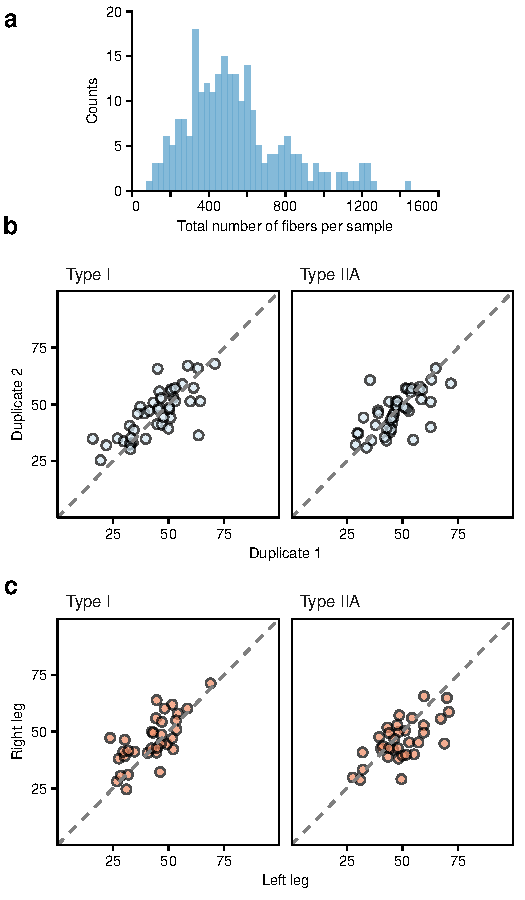
\includegraphics{thesis_files/figure-latex/fiber-methods-fig-1} 

}

\caption[Characteristics of biopsy samples used in immunohistochemistry analyses.]{Number of fibres in immunohistochemistry analyses (a), correlation between duplicate samples from the same leg (separated by 2 hours) (b) and correlations between samples from left and right leg pre-intervention.}\label{fig:fiber-methods-fig}
\end{figure}
In Study I, one or several pieces of muscle (total weight
\(\sim\)\SI{15}{mg}) were chosen per sampling for analysis of fiber type
composition. The average total number of counted fibers per samples was 539.
Only a small percentage (5.4\%) of samples did not contain enough fibers for representative analysis of fiber type composition (\textgreater{} 200 fibers)
{[}321{]}
and as many as 1400 fibers were counted in some specimens (\ref{fig:fiber-methods-fig}a).
The smaller amount of tissue obtained using the micro-biopsy technique did thus not limit analyses of fiber type composition.

In order to asses the reproducibility of the technique, samples obtained during the same day (separated by \(\sim\) 2 hours) were analyzed as duplicate samples.
Standard deviations from duplicate measures were calculated as by Blomstrand \emph{et al.} {[}321{]}

\[SD = \sqrt{\frac{\sum{d^2}}{2n}}\]
where \(d\) is the difference between paired observations and \(n\) is the number of pairs.
The variation (SD) between duplicate samples were 5.86 and 5.49 for Type I and IIA fibers, respectively (\ref{fig:fiber-methods-fig}b).
This did only marginally differ from between leg variations (Type I, 6.31; Type IIA, 6.24; Figure \ref{fig:fiber-methods-fig}c).
These estimates are slightly lower than those reported by Blomstrand \emph{et al.}, using the Bergström needle
{[}321{]}.
This suggests that the micro-biopsy technique is reproducible in terms of repeated sampling.

\hypertarget{feasibility-of-model-based-normalization-of-rt-qpcr-based-gene-expression-data-in-a-case-of-human-muscle-under-hypertrophic-stress}{%
\section{Feasibility of model-based normalization of RT-qPCR-based gene-expression data in a case of human muscle under hypertrophic stress}\label{feasibility-of-model-based-normalization-of-rt-qpcr-based-gene-expression-data-in-a-case-of-human-muscle-under-hypertrophic-stress}}

Quantitative reverse-transcription real-time polymerase chain-reaction (RT-qPCR) is the method of choice for conducting targeted gene-expression studies.
For accurate interpretation of such data the selection of normalization strategy needs to account for biological as well as non-biological variation.
Whereas analysis using endogenous control genes is the most commonly adopted approach, model-based strategies using estimates of technical variation from multiple genes could offer increased sensitivity and accuracy.\\
Here, we compare the feasibility gene-specific and model-based normalization strategies for analyzing the effect of two resistance-training programs on abundance of IGF-1 and myostatin mRNA in humans. As for gene-specific normalization, neither of the eleven commonly utilized endogenous control genes investigated exhibited stability suggesting that the use of endogenous internal controls for normalization may affect interpretation. In contrast, using mixed-effects models utilized to estimate technical variation between samples without relying on endogenous controls proved to be feasible.
Simulations further showed that model-based strategies were computationally robust and had higher power than traditional analysis.

\hypertarget{increased-relevance-of-rna-seq-data-through-data-driven-selection-of}{%
\section{Increased relevance of RNA-seq data through data-driven selection of}\label{increased-relevance-of-rna-seq-data-through-data-driven-selection-of}}

\hypertarget{conclusion}{%
\chapter*{Conclusion}\label{conclusion}}
\addcontentsline{toc}{chapter}{Conclusion}

If we don't want Conclusion to have a chapter number next to it, we can add the \texttt{\{-\}} attribute.

\textbf{More info}

And here's some other random info: the first paragraph after a chapter title or section head \emph{shouldn't be} indented, because indents are to tell the reader that you're starting a new paragraph. Since that's obvious after a chapter or section title, proper typesetting doesn't add an indent there.

\hypertarget{acknowledgements}{%
\chapter{Acknowledgements}\label{acknowledgements}}

This thesis was primarily realized at Lillehammer University College/Inland University of Applied Sciences and Sykehuset innlandet. Without the help of

Stian Ellefsen, my main supervisor during these years, I would not have been the same scientist without your enthusiasm. You have thought me that science is fun, and serious, bust mostly fun, but also serious business.

Bent R. Rønnestad, my co-supervisor

Eva Blomstrand, my co-supervisor at GIH, thank you for taking me on board and for all your support.

I am grateful for the support from The Swedish School of Sport and Health
Sciences, GIH, especially Kent Sahlin who created a spot for me in your doctorate program and Camilla Norrbin and Bim O'Reilly for keeping track on me during these years. I regret not spending more time at GIH during these years, I always felt at home Lidingövägen 1.

This thesis would not have been possible without the Jon Elling Whist

Sjur J. Øfsteng was my second office mate at Lillehammer and

Olav Vikmoen was my first office mate at Lillehammer, he speaks an peculiar dialect native to southern parts of Gudbrandsdalen. This was

Anne Grete Mathisen, help with blood sampling during training study (knitting a shirt to grandkids between sampling)
Jostein, Caroline, Anne Cecilie (study I)
to Johanne Seeberg, Stine Dahl, Marianne Bratlien, Martin Nordseth, Erlend Hakestad, Ole-Martin Hveem and Mari Skifjeld (study II)
Jon Elling Whist, Marita Hanestadhaugen, Lise Koll
Bente Malerbakken, Jostein Flata (R-sykehuset)

Knut Sindre Mølmen

Nicke W. Almquist

Joar Hansen
Eirik Grindaker
Håvard Nygaard

William Apro thaught everything I know about western blotting! Thank you for being a great mentor and meeting me at the Åstrand laboratory at 5:45 in the morning.

While working with this thesis I have been fortunate to teach at our bachelor- and master-program in sport science. I would like to thank all devoted students trying to learn Swedish while I was talking about cross-country skiing, strength testing or data science. You have undoubtedly thought me more than I have managed to accomplish in the opposite direction.

Jostein Flata, Bente Malerbakken

During my years at Lillehammer university college (later Inland University of Applied Sciences)\footnote{I do not know who came up with this name, the abbreviation does not read well in English} we planned three different labs and built one.

Thanks to all my old colleagues at Dalarna University (Anders, Tomas, Magnus, Frej, Michail, ), I hope you have not forgotten about me! Thanks to Emma Hawke for advice on life in general, science and the English language in particular.

Thanks to my Norwegian family, Torill, Eivind, Stina, Petter, Emil, Anton, Oskar, Ida, Bent, Elvira, Olava and Ingrid for supporting me and Marie during these years.

Marie, I'm sorry for all the late nights, early mornings and weekends i did not spend with you. You have supported me during this time, and we are still together, success! I love you!

\hypertarget{svensk-sammanfattning}{%
\chapter{Svensk sammanfattning}\label{svensk-sammanfattning}}

\backmatter

\hypertarget{references}{%
\chapter*{References}\label{references}}
\addcontentsline{toc}{chapter}{References}

\markboth{References}{References}

\noindent

\setlength{\parskip}{4pt}

\rightskip3em

\footnotesize

\hypertarget{refs}{}
\begin{CSLReferences}{0}{0}
\leavevmode\hypertarget{ref-RN2512}{}%
\CSLLeftMargin{{[}1{]} }
\CSLRightInline{Li R, Xia J, Zhang XI, Gathirua-Mwangi WG, Guo J, Li Y, et al. Associations of muscle mass and strength with all-cause mortality among US older adults. Medicine and Science in Sports and Exercise 2018;50:458--67. \url{https://doi.org/10.1249/MSS.0000000000001448}.}

\leavevmode\hypertarget{ref-RN2808}{}%
\CSLLeftMargin{{[}2{]} }
\CSLRightInline{García-Hermoso A, Cavero-Redondo I, Ramírez-Vélez R, Ruiz JR, Ortega FB, Lee D-C, et al. Muscular strength as a predictor of all-cause mortality in an apparently healthy population: A systematic review and meta-analysis of data from approximately 2 million men and women. Archives of Physical Medicine and Rehabilitation 2018;99:2100--2113.e5. https://doi.org/\url{https://doi.org/10.1016/j.apmr.2018.01.008}.}

\leavevmode\hypertarget{ref-RN2513}{}%
\CSLLeftMargin{{[}3{]} }
\CSLRightInline{Fukasawa H, Kaneko M, Niwa H, Matsuyama T, Yasuda H, Kumagai H, et al. Lower thigh muscle mass is associated with all-cause and cardiovascular mortality in elderly hemodialysis patients. European Journal of Clinical Nutrition 2017;71:64--9. \url{https://doi.org/10.1038/ejcn.2016.186}.}

\leavevmode\hypertarget{ref-RN2514}{}%
\CSLLeftMargin{{[}4{]} }
\CSLRightInline{Miyake H, Kanazawa I, Tanaka KI, Sugimoto T. Low skeletal muscle mass is associated with the risk of all-cause mortality in patients with type 2 diabetes mellitus. Ther Adv Endocrinol Metab 2019;10:2042018819842971. \url{https://doi.org/10.1177/2042018819842971}.}

\leavevmode\hypertarget{ref-RN2809}{}%
\CSLLeftMargin{{[}5{]} }
\CSLRightInline{Ruiz JR, Sui X, Lobelo F, Morrow JR, Jackson AW, Sjöström M, et al. Association between muscular strength and mortality in men: Prospective cohort study. BMJ 2008;337:a439. \url{https://doi.org/10.1136/bmj.a439}.}

\leavevmode\hypertarget{ref-RN2515}{}%
\CSLLeftMargin{{[}6{]} }
\CSLRightInline{Szulc P, Munoz F, Marchand F, Chapurlat R, Delmas PD. Rapid loss of appendicular skeletal muscle mass is associated with higher all-cause mortality in older men: The prospective MINOS study. Am J Clin Nutr 2010;91:1227--36. \url{https://doi.org/10.3945/ajcn.2009.28256}.}

\leavevmode\hypertarget{ref-RN2516}{}%
\CSLLeftMargin{{[}7{]} }
\CSLRightInline{Abramowitz MK, Hall CB, Amodu A, Sharma D, Androga L, Hawkins M. Muscle mass, BMI, and mortality among adults in the united states: A population-based cohort study. PLoS One 2018;13:e0194697. \url{https://doi.org/10.1371/journal.pone.0194697}.}

\leavevmode\hypertarget{ref-RN2517}{}%
\CSLLeftMargin{{[}8{]} }
\CSLRightInline{Janssen I, Heymsfield SB, Ross R. Low relative skeletal muscle mass (sarcopenia) in older persons is associated with functional impairment and physical disability. J Am Geriatr Soc 2002;50:889--96. \url{https://doi.org/10.1046/j.1532-5415.2002.50216.x}.}

\leavevmode\hypertarget{ref-RN2532}{}%
\CSLLeftMargin{{[}9{]} }
\CSLRightInline{Sousa AS, Guerra RS, Fonseca I, Pichel F, Ferreira S, Amaral TF. Financial impact of sarcopenia on hospitalization costs. Eur J Clin Nutr 2016;70:1046--51. \url{https://doi.org/10.1038/ejcn.2016.73}.}

\leavevmode\hypertarget{ref-RN2184}{}%
\CSLLeftMargin{{[}10{]} }
\CSLRightInline{Pinedo-Villanueva R, Westbury LD, Syddall HE, Sanchez-Santos MT, Dennison EM, Robinson SM, et al. Health care costs associated with muscle weakness: A UK population-based estimate. Calcif Tissue Int 2019;104:137--44. \url{https://doi.org/10.1007/s00223-018-0478-1}.}

\leavevmode\hypertarget{ref-RN763}{}%
\CSLLeftMargin{{[}11{]} }
\CSLRightInline{Wolfe RR. The underappreciated role of muscle in health and disease. Am J Clin Nutr 2006;84:475--82.}

\leavevmode\hypertarget{ref-RN2526}{}%
\CSLLeftMargin{{[}12{]} }
\CSLRightInline{Arden NK, Spector TD. Genetic influences on muscle strength, lean body mass, and bone mineral density: A twin study. Journal of Bone and Mineral Research 1997;12:2076--81. \url{https://doi.org/10.1359/jbmr.1997.12.12.2076}.}

\leavevmode\hypertarget{ref-RN2527}{}%
\CSLLeftMargin{{[}13{]} }
\CSLRightInline{Roth SM. Genetic aspects of skeletal muscle strength and mass with relevance to sarcopenia. BoneKEy Reports 2012;1:58--8. \url{https://doi.org/10.1038/bonekey.2012.58}.}

\leavevmode\hypertarget{ref-RN1741}{}%
\CSLLeftMargin{{[}14{]} }
\CSLRightInline{Ahtiainen JP, Walker S, Peltonen H, Holviala J, Sillanpaa E, Karavirta L, et al. Heterogeneity in resistance training-induced muscle strength and mass responses in men and women of different ages. Age (Dordr) 2016;38:10. \url{https://doi.org/10.1007/s11357-015-9870-1}.}

\leavevmode\hypertarget{ref-RN2534}{}%
\CSLLeftMargin{{[}15{]} }
\CSLRightInline{Grgic J, Garofolini A, Orazem J, Sabol F, Schoenfeld BJ, Pedisic Z. Effects of resistance training on muscle size and strength in very elderly adults: A systematic review and meta-analysis of randomized controlled trials. Sports Med 2020. \url{https://doi.org/10.1007/s40279-020-01331-7}.}

\leavevmode\hypertarget{ref-RN2536}{}%
\CSLLeftMargin{{[}16{]} }
\CSLRightInline{Faigenbaum AD, Myer GD. Resistance training among young athletes: Safety, efficacy and injury prevention effects. British Journal of Sports Medicine 2010;44:56. \url{https://doi.org/10.1136/bjsm.2009.068098}.}

\leavevmode\hypertarget{ref-RN1}{}%
\CSLLeftMargin{{[}17{]} }
\CSLRightInline{Ratamess N, Alvar BA, Evetoch TK, Housh TJ, Kibler B, Kraemer WJ, et al. American college of sports medicine position stand. Progression models in resistance training for healthy adults. Med Sci Sports Exerc 2009;41:687--708. \url{https://doi.org/10.1249/MSS.0b013e3181915670}.}

\leavevmode\hypertarget{ref-RN798}{}%
\CSLLeftMargin{{[}18{]} }
\CSLRightInline{Bird SP, Tarpenning KM, Marino FE. Designing resistance training programmes to enhance muscular fitness: A review of the acute programme variables. Sports Med 2005;35:841--51.}

\leavevmode\hypertarget{ref-RN2538}{}%
\CSLLeftMargin{{[}19{]} }
\CSLRightInline{Feigenbaum MS, Pollock ML. Prescription of resistance training for health and disease. Med Sci Sports Exerc 1999;31:38--45. \url{https://doi.org/10.1097/00005768-199901000-00008}.}

\leavevmode\hypertarget{ref-RN791}{}%
\CSLLeftMargin{{[}20{]} }
\CSLRightInline{Burd NA, Holwerda AM, Selby KC, West DW, Staples AW, Cain NE, et al. Resistance exercise volume affects myofibrillar protein synthesis and anabolic signalling molecule phosphorylation in young men. J Physiol 2010;588:3119--30. \url{https://doi.org/10.1113/jphysiol.2010.192856}.}

\leavevmode\hypertarget{ref-RN784}{}%
\CSLLeftMargin{{[}21{]} }
\CSLRightInline{Terzis G, Spengos K, Mascher H, Georgiadis G, Manta P, Blomstrand E. The degree of p70 S6k and S6 phosphorylation in human skeletal muscle in response to resistance exercise depends on the training volume. Eur J Appl Physiol 2010;110:835--43. \url{https://doi.org/10.1007/s00421-010-1527-2}.}

\leavevmode\hypertarget{ref-RN1837}{}%
\CSLLeftMargin{{[}22{]} }
\CSLRightInline{Ahtiainen JP, Walker S, Silvennoinen M, Kyrolainen H, Nindl BC, Hakkinen K, et al. Exercise type and volume alter signaling pathways regulating skeletal muscle glucose uptake and protein synthesis. Eur J Appl Physiol 2015;115:1835--45. \url{https://doi.org/10.1007/s00421-015-3155-3}.}

\leavevmode\hypertarget{ref-RN793}{}%
\CSLLeftMargin{{[}23{]} }
\CSLRightInline{Krieger JW. Single versus multiple sets of resistance exercise: A meta-regression. J Strength Cond Res 2009;23:1890--901. \url{https://doi.org/10.1519/JSC.0b013e3181b370be}.}

\leavevmode\hypertarget{ref-RN789}{}%
\CSLLeftMargin{{[}24{]} }
\CSLRightInline{Krieger JW. Single vs. Multiple sets of resistance exercise for muscle hypertrophy: A meta-analysis. J Strength Cond Res 2010;24:1150--9. \url{https://doi.org/10.1519/JSC.0b013e3181d4d436}.}

\leavevmode\hypertarget{ref-RN1767}{}%
\CSLLeftMargin{{[}25{]} }
\CSLRightInline{Schoenfeld BJ, Ogborn D, Krieger JW. Dose-response relationship between weekly resistance training volume and increases in muscle mass: A systematic review and meta-analysis. J Sports Sci 2016:1--0. \url{https://doi.org/10.1080/02640414.2016.1210197}.}

\leavevmode\hypertarget{ref-RN2063}{}%
\CSLLeftMargin{{[}26{]} }
\CSLRightInline{Choi J, Lee M, Lee JK, Kang D, Choi JY. Correlates associated with participation in physical activity among adults: A systematic review of reviews and update. BMC Public Health 2017;17:356. \url{https://doi.org/10.1186/s12889-017-4255-2}.}

\leavevmode\hypertarget{ref-RN794}{}%
\CSLLeftMargin{{[}27{]} }
\CSLRightInline{Carpinelli RN, Otto RM. Strength training. Single versus multiple sets. Sports Med 1998;26:73--84.}

\leavevmode\hypertarget{ref-RN2547}{}%
\CSLLeftMargin{{[}28{]} }
\CSLRightInline{Pickering C, Kiely J. Do non-responders to exercise exist---and if so, what should we do about them? Sports Medicine 2019;49:1--7. \url{https://doi.org/10.1007/s40279-018-01041-1}.}

\leavevmode\hypertarget{ref-RN2640}{}%
\CSLLeftMargin{{[}29{]} }
\CSLRightInline{Tipton CM. The history of "exercise is medicine" in ancient civilizations. Adv Physiol Educ 2014;38:109--17. \url{https://doi.org/10.1152/advan.00136.2013}.}

\leavevmode\hypertarget{ref-RN2663}{}%
\CSLLeftMargin{{[}30{]} }
\CSLRightInline{Pfister G. Cultural confrontations: German turnen, swedish gymnastics and english sport--european diversity in physical activities from a historical perspective. Culture, Sport, Society 2003;6:61--91.}

\leavevmode\hypertarget{ref-RN2634}{}%
\CSLLeftMargin{{[}31{]} }
\CSLRightInline{Nicoll EA. Principles of exercise therapy. British Medical Journal 1943;1:747--50. \url{https://doi.org/10.1136/bmj.1.4302.747}.}

\leavevmode\hypertarget{ref-RN2633}{}%
\CSLLeftMargin{{[}32{]} }
\CSLRightInline{Delorme TL. RESTORATION OF MUSCLE POWER BY HEAVY-RESISTANCE EXERCISES. JBJS 1945;27.}

\leavevmode\hypertarget{ref-RN2639}{}%
\CSLLeftMargin{{[}33{]} }
\CSLRightInline{Todd JS, Shurley JP, Todd TC. Thomas l. DeLorme and the science of progressive resistance exercise. J Strength Cond Res 2012;26:2913--23. \url{https://doi.org/10.1519/JSC.0b013e31825adcb4}.}

\leavevmode\hypertarget{ref-RN2641}{}%
\CSLLeftMargin{{[}34{]} }
\CSLRightInline{Delorme TL, Watkins AL. Technics of progressive resistance exercise. Arch Phys Med Rehabil 1948;29:263--73.}

\leavevmode\hypertarget{ref-RN2646}{}%
\CSLLeftMargin{{[}35{]} }
\CSLRightInline{Delorme TL, West FE, Shriber WJ. INFLUENCE OF PROGRESSIVE-RESISTANCE EXERCISES ON KNEE FUNCTION FOLLOWING FEMORAL FRACTURES. JBJS 1950;32.}

\leavevmode\hypertarget{ref-RN2632}{}%
\CSLLeftMargin{{[}36{]} }
\CSLRightInline{Houtz SJ, Parrish AM, Hellebrandt FA. The influence of heavy resistance exercise on strength. Physical Therapy 1946;26:299--304. \url{https://doi.org/10.1093/ptj/26.6.299}.}

\leavevmode\hypertarget{ref-RN2644}{}%
\CSLLeftMargin{{[}37{]} }
\CSLRightInline{Chui E. The effect of systematic weight training on athletic power. Research Quarterly American Association for Health, Physical Education and Recreation 1950;21:188--94. \url{https://doi.org/10.1080/10671188.1950.10624849}.}

\leavevmode\hypertarget{ref-RN2642}{}%
\CSLLeftMargin{{[}38{]} }
\CSLRightInline{Capen EK. The effect of systematic weight training on power, strength, and endurance. Research Quarterly American Association for Health, Physical Education and Recreation 1950;21:83--93. \url{https://doi.org/10.1080/10671188.1950.10624835}.}

\leavevmode\hypertarget{ref-RN2645}{}%
\CSLLeftMargin{{[}39{]} }
\CSLRightInline{Hettinger T, Müller EA. Muskelleistung und muskeltraining. Arbeitsphysiologie 1953;15:111--26. \url{https://doi.org/10.1007/BF00934143}.}

\leavevmode\hypertarget{ref-RN1477}{}%
\CSLLeftMargin{{[}40{]} }
\CSLRightInline{Capen EK. Study of four programs of heavy resistance exercises for development of muscular strength. Research Quarterly American Association for Health, Physical Education and Recreation 1956;27:132--42. \url{https://doi.org/10.1080/10671188.1956.10612864}.}

\leavevmode\hypertarget{ref-RN1472}{}%
\CSLLeftMargin{{[}41{]} }
\CSLRightInline{Galvao DA, Taaffe DR. Resistance exercise dosage in older adults: Single- versus multiset effects on physical performance and body composition. J Am Geriatr Soc 2005;53:2090--7. \url{https://doi.org/10.1111/j.1532-5415.2005.00494.x}.}

\leavevmode\hypertarget{ref-RN2659}{}%
\CSLLeftMargin{{[}42{]} }
\CSLRightInline{Berger RA. COMPARISON OF THE EFFECT OF VARIOUS WEIGHT TRAINING LOADS ON STRENGTH. Res Q 1965;36:141--6.}

\leavevmode\hypertarget{ref-RN2658}{}%
\CSLLeftMargin{{[}43{]} }
\CSLRightInline{Berger RA, Hardage B. Effect of maximum loads for each of ten repetitions on strength improvement. Res Q 1967;38:715--8.}

\leavevmode\hypertarget{ref-RN2656}{}%
\CSLLeftMargin{{[}44{]} }
\CSLRightInline{O'Shea P. Effects of selected weight training programs on the development of strength and muscle hypertrophy. Res Q 1966;37:95--102.}

\leavevmode\hypertarget{ref-RN2537}{}%
\CSLLeftMargin{{[}45{]} }
\CSLRightInline{Fleck SJ, Kraemer WJ. Designing resistance training programs. Fourth edition. Champaign, IL: Human Kinetics; 2014.}

\leavevmode\hypertarget{ref-RN2655}{}%
\CSLLeftMargin{{[}46{]} }
\CSLRightInline{American college of sports medicine position statement on the recommended quantity and quality of exercise for developing and maintaining fitness in healthy adults. Med Sci Sports 1978;10:vii--x.}

\leavevmode\hypertarget{ref-RN2654}{}%
\CSLLeftMargin{{[}47{]} }
\CSLRightInline{American college of sports medicine position stand. The recommended quantity and quality of exercise for developing and maintaining cardiorespiratory and muscular fitness in healthy adults. Med Sci Sports Exerc 1990;22:265--74.}

\leavevmode\hypertarget{ref-RN2666}{}%
\CSLLeftMargin{{[}48{]} }
\CSLRightInline{Manley AF. Physical activity and health: A report of the surgeon general. Diane Publishing; 1996.}

\leavevmode\hypertarget{ref-RN2667}{}%
\CSLLeftMargin{{[}49{]} }
\CSLRightInline{Bull FC, Al-Ansari SS, Biddle S, Borodulin K, Buman MP, Cardon G, et al. World health organization 2020 guidelines on physical activity and sedentary behaviour. British Journal of Sports Medicine 2020;54:1451--62.}

\leavevmode\hypertarget{ref-RN2696}{}%
\CSLLeftMargin{{[}50{]} }
\CSLRightInline{n.d.;2021.}

\leavevmode\hypertarget{ref-RN2678}{}%
\CSLLeftMargin{{[}51{]} }
\CSLRightInline{Sanford JA, Nogiec CD, Lindholm ME, Adkins JN, Amar D, Dasari S, et al. Molecular transducers of physical activity consortium (MoTrPAC): Mapping the dynamic responses to exercise. Cell 2020;181:1464--74. https://doi.org/\url{https://doi.org/10.1016/j.cell.2020.06.004}.}

\leavevmode\hypertarget{ref-RN2677}{}%
\CSLLeftMargin{{[}52{]} }
\CSLRightInline{Sparks LM. Exercise training response heterogeneity: Physiological and molecular insights. Diabetologia 2017;60:2329--36. \url{https://doi.org/10.1007/s00125-017-4461-6}.}

\leavevmode\hypertarget{ref-RN764}{}%
\CSLLeftMargin{{[}53{]} }
\CSLRightInline{Hubal MJ, Gordish-Dressman H, Thompson PD, Price TB, Hoffman EP, Angelopoulos TJ, et al. Variability in muscle size and strength gain after unilateral resistance training. Med Sci Sports Exerc 2005;37:964--72.}

\leavevmode\hypertarget{ref-RN1263}{}%
\CSLLeftMargin{{[}54{]} }
\CSLRightInline{Pescatello LS, Devaney JM, Hubal MJ, Thompson PD, Hoffman EP. Highlights from the functional single nucleotide polymorphisms associated with human muscle size and strength or FAMuSS study. Biomed Res Int 2013;2013:643575. \url{https://doi.org/10.1155/2013/643575}.}

\leavevmode\hypertarget{ref-RN826}{}%
\CSLLeftMargin{{[}55{]} }
\CSLRightInline{Thalacker-Mercer A, Stec M, Cui X, Cross J, Windham S, Bamman M. Cluster analysis reveals differential transcript profiles associated with resistance training-induced human skeletal muscle hypertrophy. Physiol Genomics 2013;45:499--507. \url{https://doi.org/10.1152/physiolgenomics.00167.2012}.}

\leavevmode\hypertarget{ref-RN2684}{}%
\CSLLeftMargin{{[}56{]} }
\CSLRightInline{Stokes T, Timmons JA, Crossland H, Tripp TR, Murphy K, McGlory C, et al. Molecular transducers of human skeletal muscle remodeling under different loading states. Cell Rep 2020;32:107980. \url{https://doi.org/10.1016/j.celrep.2020.107980}.}

\leavevmode\hypertarget{ref-RN2698}{}%
\CSLLeftMargin{{[}57{]} }
\CSLRightInline{Roth SM. Perspective on the future use of genomics in exercise prescription. J Appl Physiol (1985) 2008;104:1243--5. \url{https://doi.org/10.1152/japplphysiol.01000.2007}.}

\leavevmode\hypertarget{ref-RN758}{}%
\CSLLeftMargin{{[}58{]} }
\CSLRightInline{Timmons JA. Variability in training-induced skeletal muscle adaptation. J Appl Physiol (1985) 2011;110:846--53. \url{https://doi.org/10.1152/japplphysiol.00934.2010}.}

\leavevmode\hypertarget{ref-RN2681}{}%
\CSLLeftMargin{{[}59{]} }
\CSLRightInline{Hautala AJ, Kiviniemi AM, Mäkikallio TH, Kinnunen H, Nissilä S, Huikuri HV, et al. Individual differences in the responses to endurance and resistance training. Eur J Appl Physiol 2006;96:535--42. \url{https://doi.org/10.1007/s00421-005-0116-2}.}

\leavevmode\hypertarget{ref-RN2699}{}%
\CSLLeftMargin{{[}60{]} }
\CSLRightInline{Montero D, Lundby C. Refuting the myth of non-response to exercise training: 'Non-responders' do respond to higher dose of training. J Physiol 2017;595:3377--87. \url{https://doi.org/10.1113/jp273480}.}

\leavevmode\hypertarget{ref-RN346}{}%
\CSLLeftMargin{{[}61{]} }
\CSLRightInline{Wernbom M, Augustsson J, Thomeé R. The influence of frequency, intensity, volume and mode of strength training on whole muscle cross-sectional area in humans. Sports Med 2007;37:225--64.}

\leavevmode\hypertarget{ref-RN1596}{}%
\CSLLeftMargin{{[}62{]} }
\CSLRightInline{DeFreitas JM, Beck TW, Stock MS, Dillon MA, Kasishke 2nd P. R. An examination of the time course of training-induced skeletal muscle hypertrophy. Eur J Appl Physiol 2011;111:2785--90. \url{https://doi.org/10.1007/s00421-011-1905-4}.}

\leavevmode\hypertarget{ref-RN2113}{}%
\CSLLeftMargin{{[}63{]} }
\CSLRightInline{Stock MS, Mota JA, DeFranco RN, Grue KA, Jacobo AU, Chung E, et al. The time course of short-term hypertrophy in the absence of eccentric muscle damage. Eur J Appl Physiol 2017;117:989--1004. \url{https://doi.org/10.1007/s00421-017-3587-z}.}

\leavevmode\hypertarget{ref-RN2736}{}%
\CSLLeftMargin{{[}64{]} }
\CSLRightInline{Narici MV, Roi GS, Landoni L, Minetti AE, Cerretelli P. Changes in force, cross-sectional area and neural activation during strength training and detraining of the human quadriceps. Eur J Appl Physiol Occup Physiol 1989;59:310--9. \url{https://doi.org/10.1007/bf02388334}.}

\leavevmode\hypertarget{ref-RN2739}{}%
\CSLLeftMargin{{[}65{]} }
\CSLRightInline{Welle S, Totterman S, Thornton C. Effect of age on muscle hypertrophy induced by resistance training. J Gerontol A Biol Sci Med Sci 1996;51:M270--5. \url{https://doi.org/10.1093/gerona/51a.6.m270}.}

\leavevmode\hypertarget{ref-RN767}{}%
\CSLLeftMargin{{[}66{]} }
\CSLRightInline{Folland JP, Williams AG. The adaptations to strength training : Morphological and neurological contributions to increased strength. Sports Med 2007;37:145--68.}

\leavevmode\hypertarget{ref-RN2740}{}%
\CSLLeftMargin{{[}67{]} }
\CSLRightInline{Roberts BM, Nuckols G, Krieger JW. Sex differences in resistance training: A systematic review and meta-analysis. J Strength Cond Res 2020;34:1448--60. \url{https://doi.org/10.1519/jsc.0000000000003521}.}

\leavevmode\hypertarget{ref-RN752}{}%
\CSLLeftMargin{{[}68{]} }
\CSLRightInline{Peterson MD, Sen A, Gordon PM. Influence of resistance exercise on lean body mass in aging adults: A meta-analysis. Med Sci Sports Exerc 2011;43:249--58. \url{https://doi.org/10.1249/MSS.0b013e3181eb6265}.}

\leavevmode\hypertarget{ref-RN2199}{}%
\CSLLeftMargin{{[}69{]} }
\CSLRightInline{Morton RW, Murphy KT, McKellar SR, Schoenfeld BJ, Henselmans M, Helms E, et al. A systematic review, meta-analysis and meta-regression of the effect of protein supplementation on resistance training-induced gains in muscle mass and strength in healthy adults. Br J Sports Med 2018;52:376--84. \url{https://doi.org/10.1136/bjsports-2017-097608}.}

\leavevmode\hypertarget{ref-RN2745}{}%
\CSLLeftMargin{{[}70{]} }
\CSLRightInline{Lixandrao ME, Ugrinowitsch C, Berton R, Vechin FC, Conceicao MS, Damas F, et al. Magnitude of muscle strength and mass adaptations between high-load resistance training versus low-load resistance training associated with blood-flow restriction: A systematic review and meta-analysis. Sports Med 2018;48:361--78. \url{https://doi.org/10.1007/s40279-017-0795-y}.}

\leavevmode\hypertarget{ref-RN2741}{}%
\CSLLeftMargin{{[}71{]} }
\CSLRightInline{Murach KA, Dungan CM, Peterson CA, McCarthy JJ. Muscle fiber splitting is a physiological response to extreme loading in animals. Exerc Sport Sci Rev 2019;47:108--15. \url{https://doi.org/10.1249/jes.0000000000000181}.}

\leavevmode\hypertarget{ref-RN2742}{}%
\CSLLeftMargin{{[}72{]} }
\CSLRightInline{Sjöström M, Lexell J, Eriksson A, Taylor CC. Evidence of fibre hyperplasia in human skeletal muscles from healthy young men? A left-right comparison of the fibre number in whole anterior tibialis muscles. Eur J Appl Physiol Occup Physiol 1991;62:301--4. \url{https://doi.org/10.1007/bf00634963}.}

\leavevmode\hypertarget{ref-RN2754}{}%
\CSLLeftMargin{{[}73{]} }
\CSLRightInline{MacDougall JD, Sale DG, Alway SE, Sutton JR. Muscle fiber number in biceps brachii in bodybuilders and control subjects. J Appl Physiol Respir Environ Exerc Physiol 1984;57:1399--403. \url{https://doi.org/10.1152/jappl.1984.57.5.1399}.}

\leavevmode\hypertarget{ref-RN2731}{}%
\CSLLeftMargin{{[}74{]} }
\CSLRightInline{Lüthi JM, Howald H, Claassen H, Rösler K, Vock P, Hoppeler H. Structural changes in skeletal muscle tissue with heavy-resistance exercise. Int J Sports Med 1986;7:123--7. \url{https://doi.org/10.1055/s-2008-1025748}.}

\leavevmode\hypertarget{ref-RN2756}{}%
\CSLLeftMargin{{[}75{]} }
\CSLRightInline{Sweeney HL, Hammers DW. Muscle contraction. Cold Spring Harb Perspect Biol 2018;10. \url{https://doi.org/10.1101/cshperspect.a023200}.}

\leavevmode\hypertarget{ref-RN2669}{}%
\CSLLeftMargin{{[}76{]} }
\CSLRightInline{Straight CR, Fedewa MV, Toth MJ, Miller MS. Improvements in skeletal muscle fiber size with resistance training are age-dependent in older adults: A systematic review and meta-analysis. Journal of Applied Physiology 2020;129:392--403. \url{https://doi.org/10.1152/japplphysiol.00170.2020}.}

\leavevmode\hypertarget{ref-RN2758}{}%
\CSLLeftMargin{{[}77{]} }
\CSLRightInline{Bamman MM, Newcomer BR, Larson-Meyer DE, Weinsier RL, Hunter GR. Evaluation of the strength-size relationship in vivo using various muscle size indices. Med Sci Sports Exerc 2000;32:1307--13. \url{https://doi.org/10.1097/00005768-200007000-00019}.}

\leavevmode\hypertarget{ref-RN1142}{}%
\CSLLeftMargin{{[}78{]} }
\CSLRightInline{Erskine RM, Fletcher G, Folland JP. The contribution of muscle hypertrophy to strength changes following resistance training. Eur J Appl Physiol 2014. \url{https://doi.org/10.1007/s00421-014-2855-4}.}

\leavevmode\hypertarget{ref-RN2629}{}%
\CSLLeftMargin{{[}79{]} }
\CSLRightInline{Ikai M, Fukunaga T. A study on training effect on strength per unit cross-sectional area of muscle by means of ultrasonic measurement. Int Z Angew Physiol 1970;28:173--80. \url{https://doi.org/10.1007/bf00696025}.}

\leavevmode\hypertarget{ref-RN2737}{}%
\CSLLeftMargin{{[}80{]} }
\CSLRightInline{Young A, Stokes M, Round JM, Edwards RH. The effect of high-resistance training on the strength and cross-sectional area of the human quadriceps. Eur J Clin Invest 1983;13:411--7. \url{https://doi.org/10.1111/j.1365-2362.1983.tb00122.x}.}

\leavevmode\hypertarget{ref-RN2735}{}%
\CSLLeftMargin{{[}81{]} }
\CSLRightInline{Narici MV, Hoppeler H, Kayser B, Landoni L, Claassen H, Gavardi C, et al. Human quadriceps cross-sectional area, torque and neural activation during 6 months strength training. Acta Physiol Scand 1996;157:175--86. \url{https://doi.org/10.1046/j.1365-201X.1996.483230000.x}.}

\leavevmode\hypertarget{ref-RN2158}{}%
\CSLLeftMargin{{[}82{]} }
\CSLRightInline{Vigotsky AD, Schoenfeld BJ, Than C, Brown JM. Methods matter: The relationship between strength and hypertrophy depends on methods of measurement and analysis. PeerJ 2018;6:e5071. \url{https://doi.org/10.7717/peerj.5071}.}

\leavevmode\hypertarget{ref-RN2760}{}%
\CSLLeftMargin{{[}83{]} }
\CSLRightInline{Mattocks KT, Buckner SL, Jessee MB, Dankel SJ, Mouser JG, Loenneke JP. Practicing the test produces strength equivalent to higher volume training. Med Sci Sports Exerc 2017;49:1945--54. \url{https://doi.org/10.1249/mss.0000000000001300}.}

\leavevmode\hypertarget{ref-RN2219}{}%
\CSLLeftMargin{{[}84{]} }
\CSLRightInline{Carroll TJ, Herbert RD, Munn J, Lee M, Gandevia SC. Contralateral effects of unilateral strength training: Evidence and possible mechanisms. J Appl Physiol (1985) 2006;101:1514--22. \url{https://doi.org/10.1152/japplphysiol.00531.2006}.}

\leavevmode\hypertarget{ref-RN2766}{}%
\CSLLeftMargin{{[}85{]} }
\CSLRightInline{Green LA, Gabriel DA. The cross education of strength and skill following unilateral strength training in the upper and lower limbs. J Neurophysiol 2018;120:468--79. \url{https://doi.org/10.1152/jn.00116.2018}.}

\leavevmode\hypertarget{ref-RN2767}{}%
\CSLLeftMargin{{[}86{]} }
\CSLRightInline{Zijdewind I, Toering ST, Bessem B, Van Der Laan O, Diercks RL. Effects of imagery motor training on torque production of ankle plantar flexor muscles. Muscle Nerve 2003;28:168--73. \url{https://doi.org/10.1002/mus.10406}.}

\leavevmode\hypertarget{ref-RN2763}{}%
\CSLLeftMargin{{[}87{]} }
\CSLRightInline{Del Vecchio A, Casolo A, Negro F, Scorcelletti M, Bazzucchi I, Enoka R, et al. The increase in muscle force after 4~weeks of strength training is mediated by adaptations in motor unit recruitment and rate coding. J Physiol 2019;597:1873--87. \url{https://doi.org/10.1113/jp277250}.}

\leavevmode\hypertarget{ref-RN2764}{}%
\CSLLeftMargin{{[}88{]} }
\CSLRightInline{Gardiner P, Dai Y, Heckman CJ. Effects of exercise training on alpha-motoneurons. J Appl Physiol (1985) 2006;101:1228--36. \url{https://doi.org/10.1152/japplphysiol.00482.2006}.}

\leavevmode\hypertarget{ref-RN819}{}%
\CSLLeftMargin{{[}89{]} }
\CSLRightInline{Schiaffino S, Reggiani C. Fiber types in mammalian skeletal muscles. Physiol Rev 2011;91:1447--531. \url{https://doi.org/10.1152/physrev.00031.2010}.}

\leavevmode\hypertarget{ref-RN846}{}%
\CSLLeftMargin{{[}90{]} }
\CSLRightInline{Harridge SD, Bottinelli R, Canepari M, Pellegrino MA, Reggiani C, Esbjornsson M, et al. Whole-muscle and single-fibre contractile properties and myosin heavy chain isoforms in humans. Pflugers Arch 1996;432:913--20.}

\leavevmode\hypertarget{ref-RN2169}{}%
\CSLLeftMargin{{[}91{]} }
\CSLRightInline{Widrick JJ, Stelzer JE, Shoepe TC, Garner DP. Functional properties of human muscle fibers after short-term resistance exercise training. Am J Physiol Regul Integr Comp Physiol 2002;283:R408--16. \url{https://doi.org/10.1152/ajpregu.00120.2002}.}

\leavevmode\hypertarget{ref-RN849}{}%
\CSLLeftMargin{{[}92{]} }
\CSLRightInline{Lionikas A, Li M, Larsson L. Human skeletal muscle myosin function at physiological and non-physiological temperatures. Acta Physiol (Oxf) 2006;186:151--8. \url{https://doi.org/10.1111/j.1748-1716.2005.01516.x}.}

\leavevmode\hypertarget{ref-RN1885}{}%
\CSLLeftMargin{{[}93{]} }
\CSLRightInline{Essen B, Jansson E, Henriksson J, Taylor AW, Saltin B. Metabolic characteristics of fibre types in human skeletal muscle. Acta Physiol Scand 1975;95:153--65. \url{https://doi.org/10.1111/j.1748-1716.1975.tb10038.x}.}

\leavevmode\hypertarget{ref-RN2801}{}%
\CSLLeftMargin{{[}94{]} }
\CSLRightInline{Karatzaferi C, Haan A de, Mechelen W van, Sargeant AJ. Metabolism changes in single human fibres during brief maximal exercise. Exp Physiol 2001;86:411--5. \url{https://doi.org/10.1113/eph8602223}.}

\leavevmode\hypertarget{ref-RN2798}{}%
\CSLLeftMargin{{[}95{]} }
\CSLRightInline{Simoneau JA, Bouchard C. Genetic determinism of fiber type proportion in human skeletal muscle. Faseb j 1995;9:1091--5. \url{https://doi.org/10.1096/fasebj.9.11.7649409}.}

\leavevmode\hypertarget{ref-RN2795}{}%
\CSLLeftMargin{{[}96{]} }
\CSLRightInline{Simoneau JA, Bouchard C. Human variation in skeletal muscle fiber-type proportion and enzyme activities. Am J Physiol 1989;257:E567--72. \url{https://doi.org/10.1152/ajpendo.1989.257.4.E567}.}

\leavevmode\hypertarget{ref-RN285}{}%
\CSLLeftMargin{{[}97{]} }
\CSLRightInline{Staron RS, Hagerman FC, Hikida RS, Murray TF, Hostler DP, Crill MT, et al. Fiber type composition of the vastus lateralis muscle of young men and women. J Histochem Cytochem 2000;48:623--9.}

\leavevmode\hypertarget{ref-RN2220}{}%
\CSLLeftMargin{{[}98{]} }
\CSLRightInline{Adams GR, Hather BM, Baldwin KM, Dudley GA. Skeletal muscle myosin heavy chain composition and resistance training. J Appl Physiol (1985) 1993;74:911--5. \url{https://doi.org/10.1152/jappl.1993.74.2.911}.}

\leavevmode\hypertarget{ref-RN2799}{}%
\CSLLeftMargin{{[}99{]} }
\CSLRightInline{Williamson DL, Gallagher PM, Carroll CC, Raue U, Trappe SW. Reduction in hybrid single muscle fiber proportions with resistance training in humans. J Appl Physiol (1985) 2001;91:1955--61. \url{https://doi.org/10.1152/jappl.2001.91.5.1955}.}

\leavevmode\hypertarget{ref-RN2056}{}%
\CSLLeftMargin{{[}100{]} }
\CSLRightInline{Andersen JL, Gruschy-Knudsen T. Rapid switch-off of the human myosin heavy chain IIX gene after heavy load muscle contractions is sustained for at least four days. Scand J Med Sci Sports 2018;28:371--80. \url{https://doi.org/10.1111/sms.12914}.}

\leavevmode\hypertarget{ref-RN1489}{}%
\CSLLeftMargin{{[}101{]} }
\CSLRightInline{Ellefsen S, Vikmoen O, Zacharoff E, Rauk I, Slettalokken G, Hammarstrom D, et al. Reliable determination of training-induced alterations in muscle fiber composition in human skeletal muscle using quantitative polymerase chain reaction. Scand J Med Sci Sports 2014;24:e332--42. \url{https://doi.org/10.1111/sms.12185}.}

\leavevmode\hypertarget{ref-RN2057}{}%
\CSLLeftMargin{{[}102{]} }
\CSLRightInline{Andersen JL, Aagaard P. Myosin heavy chain IIX overshoot in human skeletal muscle. Muscle Nerve 2000;23:1095--104.}

\leavevmode\hypertarget{ref-RN2108}{}%
\CSLLeftMargin{{[}103{]} }
\CSLRightInline{Borina E, Pellegrino MA, D'Antona G, Bottinelli R. Myosin and actin content of human skeletal muscle fibers following 35 days bed rest. Scand J Med Sci Sports 2010;20:65--73. \url{https://doi.org/10.1111/j.1600-0838.2009.01029.x}.}

\leavevmode\hypertarget{ref-RN1505}{}%
\CSLLeftMargin{{[}104{]} }
\CSLRightInline{Burd NA, Andrews RJ, West DW, Little JP, Cochran AJ, Hector AJ, et al. Muscle time under tension during resistance exercise stimulates differential muscle protein sub-fractional synthetic responses in men. J Physiol 2012;590:351--62. \url{https://doi.org/10.1113/jphysiol.2011.221200}.}

\leavevmode\hypertarget{ref-RN2608}{}%
\CSLLeftMargin{{[}105{]} }
\CSLRightInline{Porter C, Reidy PT, Bhattarai N, Sidossis LS, Rasmussen BB. Resistance exercise training alters mitochondrial function in human skeletal muscle. Medicine and Science in Sports and Exercise 2015;47:1922--31. \url{https://doi.org/10.1249/MSS.0000000000000605}.}

\leavevmode\hypertarget{ref-RN2817}{}%
\CSLLeftMargin{{[}106{]} }
\CSLRightInline{Chan DC. Mitochondrial fusion and fission in mammals. Annu Rev Cell Dev Biol 2006;22:79--99. \url{https://doi.org/10.1146/annurev.cellbio.22.010305.104638}.}

\leavevmode\hypertarget{ref-RN2816}{}%
\CSLLeftMargin{{[}107{]} }
\CSLRightInline{Mishra P, Varuzhanyan G, Pham AH, Chan DC. Mitochondrial dynamics is a distinguishing feature of skeletal muscle fiber types and regulates organellar compartmentalization. Cell Metab 2015;22:1033--44. \url{https://doi.org/10.1016/j.cmet.2015.09.027}.}

\leavevmode\hypertarget{ref-RN2818}{}%
\CSLLeftMargin{{[}108{]} }
\CSLRightInline{Lin J, Wu H, Tarr PT, Zhang CY, Wu Z, Boss O, et al. Transcriptional co-activator PGC-1 alpha drives the formation of slow-twitch muscle fibres. Nature 2002;418:797--801. \url{https://doi.org/10.1038/nature00904}.}

\leavevmode\hypertarget{ref-RN2819}{}%
\CSLLeftMargin{{[}109{]} }
\CSLRightInline{Handschin C, Chin S, Li P, Liu F, Maratos-Flier E, Lebrasseur NK, et al. Skeletal muscle fiber-type switching, exercise intolerance, and myopathy in PGC-1alpha muscle-specific knock-out animals. J Biol Chem 2007;282:30014--21. \url{https://doi.org/10.1074/jbc.M704817200}.}

\leavevmode\hypertarget{ref-RN2775}{}%
\CSLLeftMargin{{[}110{]} }
\CSLRightInline{Greendale GA, Huang MH, Wang Y, Finkelstein JS, Danielson ME, Sternfeld B. Sport and home physical activity are independently associated with bone density. Med Sci Sports Exerc 2003;35:506--12. \url{https://doi.org/10.1249/01.Mss.0000056725.64347.C9}.}

\leavevmode\hypertarget{ref-RN2771}{}%
\CSLLeftMargin{{[}111{]} }
\CSLRightInline{Magnusson SP, Narici MV, Maganaris CN, Kjaer M. Human tendon behaviour and adaptation, in vivo. J Physiol 2008;586:71--81. \url{https://doi.org/10.1113/jphysiol.2007.139105}.}

\leavevmode\hypertarget{ref-RN2774}{}%
\CSLLeftMargin{{[}112{]} }
\CSLRightInline{Miller LE, Nickols-Richardson SM, Wootten DF, Ramp WK, Steele CR, Cotton JR, et al. Isokinetic resistance training increases tibial bending stiffness in young women. Calcif Tissue Int 2009;84:446--52. \url{https://doi.org/10.1007/s00223-009-9247-5}.}

\leavevmode\hypertarget{ref-RN2772}{}%
\CSLLeftMargin{{[}113{]} }
\CSLRightInline{Massey GJ, Balshaw TG, Maden-Wilkinson TM, Folland JP. Tendinous tissue properties after short- and long-term functional overload: Differences between controls, 12~weeks and 4~years of resistance training. Acta Physiol (Oxf) 2018;222:e13019. \url{https://doi.org/10.1111/apha.13019}.}

\leavevmode\hypertarget{ref-RN2770}{}%
\CSLLeftMargin{{[}114{]} }
\CSLRightInline{Kjaer M, Magnusson P, Krogsgaard M, Boysen Møller J, Olesen J, Heinemeier K, et al. Extracellular matrix adaptation of tendon and skeletal muscle to exercise. J Anat 2006;208:445--50. \url{https://doi.org/10.1111/j.1469-7580.2006.00549.x}.}

\leavevmode\hypertarget{ref-RN2783}{}%
\CSLLeftMargin{{[}115{]} }
\CSLRightInline{Borg TK, Caulfield JB. Morphology of connective tissue in skeletal muscle. Tissue Cell 1980;12:197--207. \url{https://doi.org/10.1016/0040-8166(80)90061-0}.}

\leavevmode\hypertarget{ref-RN2421}{}%
\CSLLeftMargin{{[}116{]} }
\CSLRightInline{Kjaer M. Role of extracellular matrix in adaptation of tendon and skeletal muscle to mechanical loading. Physiol Rev 2004;84:649--98. \url{https://doi.org/10.1152/physrev.00031.2003}.}

\leavevmode\hypertarget{ref-RN2788}{}%
\CSLLeftMargin{{[}117{]} }
\CSLRightInline{Miller BF, Olesen JL, Hansen M, Døssing S, Crameri RM, Welling RJ, et al. Coordinated collagen and muscle protein synthesis in human patella tendon and quadriceps muscle after exercise. J Physiol 2005;567:1021--33. \url{https://doi.org/10.1113/jphysiol.2005.093690}.}

\leavevmode\hypertarget{ref-RN2454}{}%
\CSLLeftMargin{{[}118{]} }
\CSLRightInline{Holm L, Hall G van, Rose AJ, Miller BF, Doessing S, Richter EA, et al. Contraction intensity and feeding affect collagen and myofibrillar protein synthesis rates differently in human skeletal muscle. Am J Physiol Endocrinol Metab 2010;298:E257--69. \url{https://doi.org/10.1152/ajpendo.00609.2009}.}

\leavevmode\hypertarget{ref-RN2298}{}%
\CSLLeftMargin{{[}119{]} }
\CSLRightInline{Damas F, Ugrinowitsch C, Libardi CA, Jannig PR, Hector AJ, McGlory C, et al. Resistance training in young men induces muscle transcriptome-wide changes associated with muscle structure and metabolism refining the response to exercise-induced stress. Eur J Appl Physiol 2018;118:2607--16. \url{https://doi.org/10.1007/s00421-018-3984-y}.}

\leavevmode\hypertarget{ref-RN774}{}%
\CSLLeftMargin{{[}120{]} }
\CSLRightInline{Raue U, Trappe TA, Estrem ST, Qian HR, Helvering LM, Smith RC, et al. Transcriptome signature of resistance exercise adaptations: Mixed muscle and fiber type specific profiles in young and old adults. J Appl Physiol (1985) 2012;112:1625--36. \url{https://doi.org/10.1152/japplphysiol.00435.2011}.}

\leavevmode\hypertarget{ref-RN2457}{}%
\CSLLeftMargin{{[}121{]} }
\CSLRightInline{Moore DR, Phillips SM, Babraj JA, Smith K, Rennie MJ. Myofibrillar and collagen protein synthesis in human skeletal muscle in young men after maximal shortening and lengthening contractions. Am J Physiol Endocrinol Metab 2005;288:E1153--9. \url{https://doi.org/10.1152/ajpendo.00387.2004}.}

\leavevmode\hypertarget{ref-RN1504}{}%
\CSLLeftMargin{{[}122{]} }
\CSLRightInline{Erskine RM, Jones DA, Maffulli N, Williams AG, Stewart CE, Degens H. What causes in vivo muscle specific tension to increase following resistance training? Exp Physiol 2011;96:145--55. \url{https://doi.org/10.1113/expphysiol.2010.053975}.}

\leavevmode\hypertarget{ref-RN2575}{}%
\CSLLeftMargin{{[}123{]} }
\CSLRightInline{Evans JW. Periodized resistance training for enhancing skeletal muscle hypertrophy and strength: A mini-review. Frontiers in Physiology 2019;10:13--3. \url{https://doi.org/10.3389/fphys.2019.00013}.}

\leavevmode\hypertarget{ref-RN2572}{}%
\CSLLeftMargin{{[}124{]} }
\CSLRightInline{Grgic J, Mikulic P, Podnar H, Pedisic Z. Effects of linear and daily undulating periodized resistance training programs on measures of muscle hypertrophy: A systematic review and meta-analysis. PeerJ 2017;5:e3695--5. \url{https://doi.org/10.7717/peerj.3695}.}

\leavevmode\hypertarget{ref-RN2571}{}%
\CSLLeftMargin{{[}125{]} }
\CSLRightInline{Schoenfeld BJ, Ogborn D, Krieger JW. Effects of resistance training frequency on measures of muscle hypertrophy: A systematic review and meta-analysis. Sports Med 2016;46:1689--97. \url{https://doi.org/10.1007/s40279-016-0543-8}.}

\leavevmode\hypertarget{ref-RN2569}{}%
\CSLLeftMargin{{[}126{]} }
\CSLRightInline{Schoenfeld BJ, Grgic J, Ogborn D, Krieger JW. Strength and hypertrophy adaptations between low- vs. High-load resistance training: A systematic review and meta-analysis. J Strength Cond Res 2017;31:3508--23. \url{https://doi.org/10.1519/jsc.0000000000002200}.}

\leavevmode\hypertarget{ref-RN1612}{}%
\CSLLeftMargin{{[}127{]} }
\CSLRightInline{Schoenfeld BJ, Ratamess NA, Peterson MD, Contreras B, Sonmez GT, Alvar BA. Effects of different volume-equated resistance training loading strategies on muscular adaptations in well-trained men. J Strength Cond Res 2014;28:2909--18. \url{https://doi.org/10.1519/JSC.0000000000000480}.}

\leavevmode\hypertarget{ref-RN2570}{}%
\CSLLeftMargin{{[}128{]} }
\CSLRightInline{Grgic J, Schoenfeld BJ, Davies TB, Lazinica B, Krieger JW, Pedisic Z. Effect of resistance training frequency on gains in muscular strength: A systematic review and meta-analysis. Sports Med 2018;48:1207--20. \url{https://doi.org/10.1007/s40279-018-0872-x}.}

\leavevmode\hypertarget{ref-RN2591}{}%
\CSLLeftMargin{{[}129{]} }
\CSLRightInline{Nunes JP, Grgic J, Cunha PM, Ribeiro AS, Schoenfeld BJ, Salles BF de, et al. What influence does resistance exercise order have on muscular strength gains and muscle hypertrophy? A systematic review and meta-analysis. Eur J Sport Sci 2020:1--9. \url{https://doi.org/10.1080/17461391.2020.1733672}.}

\leavevmode\hypertarget{ref-RN2492}{}%
\CSLLeftMargin{{[}130{]} }
\CSLRightInline{Ralston GW, Kilgore L, Wyatt FB, Baker JS. The effect of weekly set volume on strength gain: A meta-analysis. Sports Med 2017;47:2585--601. \url{https://doi.org/10.1007/s40279-017-0762-7}.}

\leavevmode\hypertarget{ref-RN2130}{}%
\CSLLeftMargin{{[}131{]} }
\CSLRightInline{Baz-Valle E, Fontes-Villalba M, Santos-Concejero J. Total number of sets as a training volume quantification method for muscle hypertrophy: A systematic review. J Strength Cond Res 2018. \url{https://doi.org/10.1519/jsc.0000000000002776}.}

\leavevmode\hypertarget{ref-RN1476}{}%
\CSLLeftMargin{{[}132{]} }
\CSLRightInline{Berger R. Effect of varied weight training programs on strength. Research Quarterly American Association for Health, Physical Education and Recreation 1962;33:168--81. \url{https://doi.org/10.1080/10671188.1962.10613188}.}

\leavevmode\hypertarget{ref-RN2568}{}%
\CSLLeftMargin{{[}133{]} }
\CSLRightInline{Junyoung H, Corinna NR, John DS, Sukho L. Low volume progressive single set of resistance training is as effective as high volume multiple sets of resistance protocol on muscle strength and power. International Journal of Applied Sports Sciences : IJASS 2015;27:33--42. \url{https://doi.org/10.24985/ijass.2015.27.1.33}.}

\leavevmode\hypertarget{ref-RN2201}{}%
\CSLLeftMargin{{[}134{]} }
\CSLRightInline{Carpinelli RN. Science versus opinion. British Journal of Sports Medicine 2004;38:240--2. \url{https://doi.org/10.1136/bjsm.2003.010710}.}

\leavevmode\hypertarget{ref-RN2465}{}%
\CSLLeftMargin{{[}135{]} }
\CSLRightInline{Ribeiro AS, Schoenfeld BJ, Pina FLC, Souza MF, Nascimento MA, Santos L dos, et al. Resistance training in older women: Comparison of single vs. Multiple sets on muscle strength and body composition. Isokinetics and Exercise Science 2015;23:53--60. \url{https://doi.org/10.3233/IES-140564}.}

\leavevmode\hypertarget{ref-RN2464}{}%
\CSLLeftMargin{{[}136{]} }
\CSLRightInline{Correa CS, Teixeira BC, Cobos RC, Macedo RC, Kruger RL, Carteri RB, et al. High-volume resistance training reduces postprandial lipaemia in postmenopausal women. J Sports Sci 2015;33:1890--901. \url{https://doi.org/10.1080/02640414.2015.1017732}.}

\leavevmode\hypertarget{ref-RN2463}{}%
\CSLLeftMargin{{[}137{]} }
\CSLRightInline{Bottaro M, Veloso J, Wagner D, Gentil P. Resistance training for strength and muscle thickness: Effect of number of sets and muscle group trained. Science \& Sports 2011;26:259--64. https://doi.org/\url{https://doi.org/10.1016/j.scispo.2010.09.009}.}

\leavevmode\hypertarget{ref-RN1570}{}%
\CSLLeftMargin{{[}138{]} }
\CSLRightInline{Radaelli R, Fleck SJ, Leite T, Leite RD, Pinto RS, Fernandes L, et al. Dose response of 1, 3 and 5 sets of resistance exercise on strength, local muscular endurance and hypertrophy. J Strength Cond Res 2014. \url{https://doi.org/10.1519/JSC.0000000000000758}.}

\leavevmode\hypertarget{ref-RN1518}{}%
\CSLLeftMargin{{[}139{]} }
\CSLRightInline{Radaelli R, Wilhelm EN, Botton CE, Rech A, Bottaro M, Brown LE, et al. Effects of single vs. Multiple-set short-term strength training in elderly women. Age (Dordr) 2014;36:9720. \url{https://doi.org/10.1007/s11357-014-9720-6}.}

\leavevmode\hypertarget{ref-RN1474}{}%
\CSLLeftMargin{{[}140{]} }
\CSLRightInline{McBride JM, Blaak JB, Triplett-McBride T. Effect of resistance exercise volume and complexity on EMG, strength, and regional body composition. Eur J Appl Physiol 2003;90:626--32. \url{https://doi.org/10.1007/s00421-003-0930-3}.}

\leavevmode\hypertarget{ref-RN1456}{}%
\CSLLeftMargin{{[}141{]} }
\CSLRightInline{Starkey DB, Pollock ML, Ishida Y, Welsch MA, Brechue WF, Graves JE, et al. Effect of resistance training volume on strength and muscle thickness. Med Sci Sports Exerc 1996;28:1311--20. \url{https://doi.org/10.1097/00005768-199610000-00016}.}

\leavevmode\hypertarget{ref-RN1454}{}%
\CSLLeftMargin{{[}142{]} }
\CSLRightInline{Ostrowski KJ, Wilson GJ, Weatherby R, Murphy PW, Lyttle AD. The effect of weight training volume on hormonal output and muscular size and function. Journal of Strength and Conditioning Research 1997;11:148--54. \url{https://doi.org/Doi\%2010.1519/00124278-199708000-00003}.}

\leavevmode\hypertarget{ref-RN1384}{}%
\CSLLeftMargin{{[}143{]} }
\CSLRightInline{Rhea MR, Alvar BA, Ball SD, Burkett LN. Three sets of weight training superior to 1 set with equal intensity for eliciting strength. J Strength Cond Res 2002;16:525--9.}

\leavevmode\hypertarget{ref-RN1382}{}%
\CSLLeftMargin{{[}144{]} }
\CSLRightInline{Cannon J, Marino FE. Early-phase neuromuscular adaptations to high- and low-volume resistance training in untrained young and older women. J Sports Sci 2010;28:1505--14. \url{https://doi.org/10.1080/02640414.2010.517544}.}

\leavevmode\hypertarget{ref-RN776}{}%
\CSLLeftMargin{{[}145{]} }
\CSLRightInline{Ronnestad BR, Egeland W, Kvamme NH, Refsnes PE, Kadi F, Raastad T. Dissimilar effects of one- and three-set strength training on strength and muscle mass gains in upper and lower body in untrained subjects. J Strength Cond Res 2007;21:157--63. \url{https://doi.org/10.1519/00124278-200702000-00028}.}

\leavevmode\hypertarget{ref-RN834}{}%
\CSLLeftMargin{{[}146{]} }
\CSLRightInline{Mitchell CJ, Churchward-Venne TA, West DW, Burd NA, Breen L, Baker SK, et al. Resistance exercise load does not determine training-mediated hypertrophic gains in young men. J Appl Physiol (1985) 2012;113:71--7. \url{https://doi.org/10.1152/japplphysiol.00307.2012}.}

\leavevmode\hypertarget{ref-RN1607}{}%
\CSLLeftMargin{{[}147{]} }
\CSLRightInline{Sooneste H, Tanimoto M, Kakigi R, Saga N, Katamoto S. Effects of training volume on strength and hypertrophy in young men. J Strength Cond Res 2013;27:8--13. \url{https://doi.org/10.1519/JSC.0b013e3182679215}.}

\leavevmode\hypertarget{ref-RN2710}{}%
\CSLLeftMargin{{[}148{]} }
\CSLRightInline{Dreyer HC, Fujita S, Cadenas JG, Chinkes DL, Volpi E, Rasmussen BB. Resistance exercise increases AMPK activity and reduces 4E-BP1 phosphorylation and protein synthesis in human skeletal muscle. The Journal of Physiology 2006;576:613--24. https://doi.org/\url{https://doi.org/10.1113/jphysiol.2006.113175}.}

\leavevmode\hypertarget{ref-RN2711}{}%
\CSLLeftMargin{{[}149{]} }
\CSLRightInline{MacDougall JD, Gibala MJ, Tarnopolsky MA, MacDonald JR, Interisano SA, Yarasheski KE. The time course for elevated muscle protein synthesis following heavy resistance exercise. Can J Appl Physiol 1995;20:480--6. \url{https://doi.org/10.1139/h95-038}.}

\leavevmode\hypertarget{ref-RN786}{}%
\CSLLeftMargin{{[}150{]} }
\CSLRightInline{Phillips SM, Tipton KD, Aarsland A, Wolf SE, Wolfe RR. Mixed muscle protein synthesis and breakdown after resistance exercise in humans. Am J Physiol 1997;273:E99--107.}

\leavevmode\hypertarget{ref-RN2712}{}%
\CSLLeftMargin{{[}151{]} }
\CSLRightInline{Biolo G, Maggi SP, Williams BD, Tipton KD, Wolfe RR. Increased rates of muscle protein turnover and amino acid transport after resistance exercise in humans. Am J Physiol 1995;268:E514--20. \url{https://doi.org/10.1152/ajpendo.1995.268.3.E514}.}

\leavevmode\hypertarget{ref-RN2717}{}%
\CSLLeftMargin{{[}152{]} }
\CSLRightInline{Chesley A, MacDougall JD, Tarnopolsky MA, Atkinson SA, Smith K. Changes in human muscle protein synthesis after resistance exercise. J Appl Physiol (1985) 1992;73:1383--8. \url{https://doi.org/10.1152/jappl.1992.73.4.1383}.}

\leavevmode\hypertarget{ref-RN1521}{}%
\CSLLeftMargin{{[}153{]} }
\CSLRightInline{Kim PL, Staron RS, Phillips SM. Fasted-state skeletal muscle protein synthesis after resistance exercise is altered with training. J Physiol 2005;568:283--90. \url{https://doi.org/10.1113/jphysiol.2005.093708}.}

\leavevmode\hypertarget{ref-RN2713}{}%
\CSLLeftMargin{{[}154{]} }
\CSLRightInline{Phillips SM, Tipton KD, Ferrando AA, Wolfe RR. Resistance training reduces the acute exercise-induced increase in muscle protein turnover. Am J Physiol 1999;276:E118--24. \url{https://doi.org/10.1152/ajpendo.1999.276.1.E118}.}

\leavevmode\hypertarget{ref-RN2714}{}%
\CSLLeftMargin{{[}155{]} }
\CSLRightInline{Børsheim E, Tipton KD, Wolf SE, Wolfe RR. Essential amino acids and muscle protein recovery from resistance exercise. Am J Physiol Endocrinol Metab 2002;283:E648--57. \url{https://doi.org/10.1152/ajpendo.00466.2001}.}

\leavevmode\hypertarget{ref-RN2715}{}%
\CSLLeftMargin{{[}156{]} }
\CSLRightInline{Tipton KD, Ferrando AA, Phillips SM, Doyle Jr D., Wolfe RR. Postexercise net protein synthesis in human muscle from orally administered amino acids. Am J Physiol 1999;276:E628--34. \url{https://doi.org/10.1152/ajpendo.1999.276.4.E628}.}

\leavevmode\hypertarget{ref-RN866}{}%
\CSLLeftMargin{{[}157{]} }
\CSLRightInline{Baar K, Esser K. Phosphorylation of p70(S6k) correlates with increased skeletal muscle mass following resistance exercise. Am J Physiol 1999;276:C120--7.}

\leavevmode\hypertarget{ref-RN860}{}%
\CSLLeftMargin{{[}158{]} }
\CSLRightInline{Kubica N, Bolster DR, Farrell PA, Kimball SR, Jefferson LS. Resistance exercise increases muscle protein synthesis and translation of eukaryotic initiation factor 2Bepsilon mRNA in a mammalian target of rapamycin-dependent manner. J Biol Chem 2005;280:7570--80. \url{https://doi.org/10.1074/jbc.M413732200}.}

\leavevmode\hypertarget{ref-RN1866}{}%
\CSLLeftMargin{{[}159{]} }
\CSLRightInline{Wilkinson SB, Phillips SM, Atherton PJ, Patel R, Yarasheski KE, Tarnopolsky MA, et al. Differential effects of resistance and endurance exercise in the fed state on signalling molecule phosphorylation and protein synthesis in human muscle. J Physiol 2008;586:3701--17. \url{https://doi.org/10.1113/jphysiol.2008.153916}.}

\leavevmode\hypertarget{ref-RN1897}{}%
\CSLLeftMargin{{[}160{]} }
\CSLRightInline{Reidy PT, Borack MS, Markofski MM, Dickinson JM, Fry CS, Deer RR, et al. Post-absorptive muscle protein turnover affects resistance training hypertrophy. Eur J Appl Physiol 2017;117:853--66. \url{https://doi.org/10.1007/s00421-017-3566-4}.}

\leavevmode\hypertarget{ref-RN1912}{}%
\CSLLeftMargin{{[}161{]} }
\CSLRightInline{Figueiredo VC, McCarthy JJ. The role of ribosome biogenesis in skeletal muscle hypertrophy. In: Sakuma K, editor. The plasticity of skeletal muscle, Singapore: Springer Singapore; 2017, p. 141--53. \url{https://doi.org/10.1007/978-981-10-3292-9_6}.}

\leavevmode\hypertarget{ref-RN2054}{}%
\CSLLeftMargin{{[}162{]} }
\CSLRightInline{Zak R, Rabinowitz M, Platt C. Ribonucleic acids associated with myofibrils. Biochemistry 1967;6:2493--9.}

\leavevmode\hypertarget{ref-RN2223}{}%
\CSLLeftMargin{{[}163{]} }
\CSLRightInline{Young VR. CHAPTER 40 - the role of skeletal and cardiac muscle in the regulation of protein metabolism. In: Munro HN, editor. Mammalian protein metabolism, Academic Press; 1970, p. 585--674. https://doi.org/\url{https://doi.org/10.1016/B978-0-12-510604-7.50018-9}.}

\leavevmode\hypertarget{ref-RN2145}{}%
\CSLLeftMargin{{[}164{]} }
\CSLRightInline{Millward DJ, Garlick PJ, James WPT, Nnanyelugo DO, Ryatt JS. Relationship between protein synthesis and RNA content in skeletal muscle. Nature 1973;241:204. \url{https://doi.org/10.1038/241204a0}.}

\leavevmode\hypertarget{ref-RN1049}{}%
\CSLLeftMargin{{[}165{]} }
\CSLRightInline{Goodman CA. The role of mTORC1 in regulating protein synthesis and skeletal muscle mass in response to various mechanical stimuli. Rev Physiol Biochem Pharmacol 2014. \url{https://doi.org/10.1007/112_2013_17}.}

\leavevmode\hypertarget{ref-RN782}{}%
\CSLLeftMargin{{[}166{]} }
\CSLRightInline{Bodine SC, Stitt TN, Gonzalez M, Kline WO, Stover GL, Bauerlein R, et al. Akt/mTOR pathway is a crucial regulator of skeletal muscle hypertrophy and can prevent muscle atrophy in vivo. Nat Cell Biol 2001;3:1014--9. \url{https://doi.org/10.1038/ncb1101-1014}.}

\leavevmode\hypertarget{ref-RN1072}{}%
\CSLLeftMargin{{[}167{]} }
\CSLRightInline{Goodman CA, Frey JW, Mabrey DM, Jacobs BL, Lincoln HC, You JS, et al. The role of skeletal muscle mTOR in the regulation of mechanical load-induced growth. J Physiol 2011;589:5485--501. \url{https://doi.org/10.1113/jphysiol.2011.218255}.}

\leavevmode\hypertarget{ref-RN785}{}%
\CSLLeftMargin{{[}168{]} }
\CSLRightInline{Terzis G, Georgiadis G, Stratakos G, Vogiatzis I, Kavouras S, Manta P, et al. Resistance exercise-induced increase in muscle mass correlates with p70S6 kinase phosphorylation in human subjects. Eur J Appl Physiol 2008;102:145--52. \url{https://doi.org/10.1007/s00421-007-0564-y}.}

\leavevmode\hypertarget{ref-RN780}{}%
\CSLLeftMargin{{[}169{]} }
\CSLRightInline{Drummond MJ, Fry CS, Glynn EL, Dreyer HC, Dhanani S, Timmerman KL, et al. Rapamycin administration in humans blocks the contraction-induced increase in skeletal muscle protein synthesis. J Physiol 2009;587:1535--46. \url{https://doi.org/10.1113/jphysiol.2008.163816}.}

\leavevmode\hypertarget{ref-RN781}{}%
\CSLLeftMargin{{[}170{]} }
\CSLRightInline{Dickinson JM, Fry CS, Drummond MJ, Gundermann DM, Walker DK, Glynn EL, et al. Mammalian target of rapamycin complex 1 activation is required for the stimulation of human skeletal muscle protein synthesis by essential amino acids. J Nutr 2011;141:856--62. \url{https://doi.org/10.3945/jn.111.139485}.}

\leavevmode\hypertarget{ref-RN2826}{}%
\CSLLeftMargin{{[}171{]} }
\CSLRightInline{Gundermann DM, Walker DK, Reidy PT, Borack MS, Dickinson JM, Volpi E, et al. Activation of mTORC1 signaling and protein synthesis in human muscle following blood flow restriction exercise is inhibited by rapamycin. Am J Physiol Endocrinol Metab 2014;306:E1198--204. \url{https://doi.org/10.1152/ajpendo.00600.2013}.}

\leavevmode\hypertarget{ref-RN2839}{}%
\CSLLeftMargin{{[}172{]} }
\CSLRightInline{Choo AY, Yoon S-O, Kim SG, Roux PP, Blenis J. Rapamycin differentially inhibits S6Ks and 4E-BP1 to mediate cell-type-specific repression of mRNA translation. Proceedings of the National Academy of Sciences 2008;105:17414. \url{https://doi.org/10.1073/pnas.0809136105}.}

\leavevmode\hypertarget{ref-RN2836}{}%
\CSLLeftMargin{{[}173{]} }
\CSLRightInline{Ogasawara R, Suginohara T. Rapamycin-insensitive mechanistic target of rapamycin regulates basal and resistance exercise-induced muscle protein synthesis. Faseb j 2018:fj201701422R. \url{https://doi.org/10.1096/fj.201701422R}.}

\leavevmode\hypertarget{ref-RN2844}{}%
\CSLLeftMargin{{[}174{]} }
\CSLRightInline{O'Neil TK, Duffy LR, Frey JW, Hornberger TA. The role of phosphoinositide 3-kinase and phosphatidic acid in the regulation of mammalian target of rapamycin following eccentric contractions. J Physiol 2009;587:3691--701. \url{https://doi.org/10.1113/jphysiol.2009.173609}.}

\leavevmode\hypertarget{ref-RN2119}{}%
\CSLLeftMargin{{[}175{]} }
\CSLRightInline{You JS, Frey JW, Hornberger TA. Mechanical stimulation induces mTOR signaling via an ERK-independent mechanism: Implications for a direct activation of mTOR by phosphatidic acid. PLoS One 2012;7:e47258. \url{https://doi.org/10.1371/journal.pone.0047258}.}

\leavevmode\hypertarget{ref-RN2126}{}%
\CSLLeftMargin{{[}176{]} }
\CSLRightInline{Fang Y, Vilella-Bach M, Bachmann R, Flanigan A, Chen J. Phosphatidic acid-mediated mitogenic activation of mTOR signaling. Science 2001;294:1942--5. \url{https://doi.org/10.1126/science.1066015}.}

\leavevmode\hypertarget{ref-RN1728}{}%
\CSLLeftMargin{{[}177{]} }
\CSLRightInline{You JS, Lincoln HC, Kim CR, Frey JW, Goodman CA, Zhong XP, et al. The role of diacylglycerol kinase zeta and phosphatidic acid in the mechanical activation of mammalian target of rapamycin (mTOR) signaling and skeletal muscle hypertrophy. J Biol Chem 2014;289:1551--63. \url{https://doi.org/10.1074/jbc.M113.531392}.}

\leavevmode\hypertarget{ref-RN2848}{}%
\CSLLeftMargin{{[}178{]} }
\CSLRightInline{Goberdhan DCI, Wilson C, Harris AL. Amino acid sensing by mTORC1: Intracellular transporters mark the spot. Cell Metabolism 2016;23:580--9. \url{https://doi.org/10.1016/j.cmet.2016.03.013}.}

\leavevmode\hypertarget{ref-RN1641}{}%
\CSLLeftMargin{{[}179{]} }
\CSLRightInline{Apro W, Moberg M, Hamilton DL, Ekblom B, Rooyackers O, Holmberg HC, et al. Leucine does not affect mechanistic target of rapamycin complex 1 assembly but is required for maximal ribosomal protein s6 kinase 1 activity in human skeletal muscle following resistance exercise. FASEB J 2015;29:4358--73. \url{https://doi.org/10.1096/fj.15-273474}.}

\leavevmode\hypertarget{ref-RN2139}{}%
\CSLLeftMargin{{[}180{]} }
\CSLRightInline{Laplante M, Sabatini DM. mTOR signaling in growth control and disease. Cell 2012;149:274--93. \url{https://doi.org/10.1016/j.cell.2012.03.017}.}

\leavevmode\hypertarget{ref-RN2837}{}%
\CSLLeftMargin{{[}181{]} }
\CSLRightInline{Gingras AC, Kennedy SG, O'Leary MA, Sonenberg N, Hay N. 4E-BP1, a repressor of mRNA translation, is phosphorylated and inactivated by the akt(PKB) signaling pathway. Genes \& Development 1998;12:502--13. \url{https://doi.org/10.1101/gad.12.4.502}.}

\leavevmode\hypertarget{ref-RN2838}{}%
\CSLLeftMargin{{[}182{]} }
\CSLRightInline{Gingras AC, Raught B, Sonenberg N. eIF4 initiation factors: Effectors of mRNA recruitment to ribosomes and regulators of translation. Annu Rev Biochem 1999;68:913--63. \url{https://doi.org/10.1146/annurev.biochem.68.1.913}.}

\leavevmode\hypertarget{ref-RN2840}{}%
\CSLLeftMargin{{[}183{]} }
\CSLRightInline{Beretta L, Gingras AC, Svitkin YV, Hall MN, Sonenberg N. Rapamycin blocks the phosphorylation of 4E-BP1 and inhibits cap-dependent initiation of translation. Embo j 1996;15:658--64.}

\leavevmode\hypertarget{ref-RN2828}{}%
\CSLLeftMargin{{[}184{]} }
\CSLRightInline{Ohanna M, Sobering AK, Lapointe T, Lorenzo L, Praud C, Petroulakis E, et al. Atrophy of S6K1(-/-) skeletal muscle cells reveals distinct mTOR effectors for cell cycle and size control. Nat Cell Biol 2005;7:286--94. \url{https://doi.org/10.1038/ncb1231}.}

\leavevmode\hypertarget{ref-RN783}{}%
\CSLLeftMargin{{[}185{]} }
\CSLRightInline{Rommel C, Bodine SC, Clarke BA, Rossman R, Nunez L, Stitt TN, et al. Mediation of IGF-1-induced skeletal myotube hypertrophy by PI(3)k/akt/mTOR and PI(3)k/akt/GSK3 pathways. Nat Cell Biol 2001;3:1009--13. \url{https://doi.org/10.1038/ncb1101-1009}.}

\leavevmode\hypertarget{ref-RN2827}{}%
\CSLLeftMargin{{[}186{]} }
\CSLRightInline{Pende M, Um SH, Mieulet V, Sticker M, Goss VL, Mestan J, et al. S6K1(-/-)/S6K2(-/-) mice exhibit perinatal lethality and rapamycin-sensitive 5'-terminal oligopyrimidine mRNA translation and reveal a mitogen-activated protein kinase-dependent S6 kinase pathway. Mol Cell Biol 2004;24:3112--24. \url{https://doi.org/10.1128/mcb.24.8.3112-3124.2004}.}

\leavevmode\hypertarget{ref-RN2321}{}%
\CSLLeftMargin{{[}187{]} }
\CSLRightInline{Chauvin C, Koka V, Nouschi A, Mieulet V, Hoareau-Aveilla C, Dreazen A, et al. Ribosomal protein S6 kinase activity controls the ribosome biogenesis transcriptional program. Oncogene 2014;33:474--83. \url{https://doi.org/10.1038/onc.2012.606}.}

\leavevmode\hypertarget{ref-RN2849}{}%
\CSLLeftMargin{{[}188{]} }
\CSLRightInline{Marabita M, Baraldo M, Solagna F, Ceelen JJM, Sartori R, Nolte H, et al. S6K1 is required for increasing skeletal muscle force during hypertrophy. Cell Rep 2016;17:501--13. \url{https://doi.org/10.1016/j.celrep.2016.09.020}.}

\leavevmode\hypertarget{ref-RN2320}{}%
\CSLLeftMargin{{[}189{]} }
\CSLRightInline{Goodman CA. Role of mTORC1 in mechanically induced increases in translation and skeletal muscle mass. Journal of Applied Physiology 2019;127:581--90. \url{https://doi.org/10.1152/japplphysiol.01011.2018}.}

\leavevmode\hypertarget{ref-RN2824}{}%
\CSLLeftMargin{{[}190{]} }
\CSLRightInline{Ruvinsky I, Meyuhas O. Ribosomal protein S6 phosphorylation: From protein synthesis to cell size. Trends Biochem Sci 2006;31:342--8. \url{https://doi.org/10.1016/j.tibs.2006.04.003}.}

\leavevmode\hypertarget{ref-RN1902}{}%
\CSLLeftMargin{{[}191{]} }
\CSLRightInline{Chiang GG, Abraham RT. Phosphorylation of mammalian target of rapamycin (mTOR) at ser-2448 is mediated by p70S6 kinase. J Biol Chem 2005;280:25485--90. \url{https://doi.org/10.1074/jbc.M501707200}.}

\leavevmode\hypertarget{ref-RN1949}{}%
\CSLLeftMargin{{[}192{]} }
\CSLRightInline{Figueiredo VC, Markworth JF, Cameron-Smith D. Considerations on mTOR regulation at serine 2448: Implications for muscle metabolism studies. Cell Mol Life Sci 2017;74:2537--45. \url{https://doi.org/10.1007/s00018-017-2481-5}.}

\leavevmode\hypertarget{ref-RN1809}{}%
\CSLLeftMargin{{[}193{]} }
\CSLRightInline{Brook MS, Wilkinson DJ, Mitchell WK, Lund JN, Phillips BE, Szewczyk NJ, et al. Synchronous deficits in cumulative muscle protein synthesis and ribosomal biogenesis underlie age-related anabolic resistance to exercise in humans. J Physiol 2016;594:7399--417. \url{https://doi.org/10.1113/JP272857}.}

\leavevmode\hypertarget{ref-RN1871}{}%
\CSLLeftMargin{{[}194{]} }
\CSLRightInline{Coffey VG, Zhong Z, Shield A, Canny BJ, Chibalin AV, Zierath JR, et al. Early signaling responses to divergent exercise stimuli in skeletal muscle from well-trained humans. Faseb j 2006;20:190--2. \url{https://doi.org/10.1096/fj.05-4809fje}.}

\leavevmode\hypertarget{ref-RN1754}{}%
\CSLLeftMargin{{[}195{]} }
\CSLRightInline{West DW, Baehr LM, Marcotte GR, Chason CM, Tolento L, Gomes AV, et al. Acute resistance exercise activates rapamycin-sensitive and -insensitive mechanisms that control translational activity and capacity in skeletal muscle. J Physiol 2016;594:453--68. \url{https://doi.org/10.1113/JP271365}.}

\leavevmode\hypertarget{ref-RN1755}{}%
\CSLLeftMargin{{[}196{]} }
\CSLRightInline{Stec MJ, Kelly NA, Many GM, Windham ST, Tuggle SC, Bamman MM. Ribosome biogenesis may augment resistance training-induced myofiber hypertrophy and is required for myotube growth in vitro. Am J Physiol Endocrinol Metab 2016;310:E652--61. \url{https://doi.org/10.1152/ajpendo.00486.2015}.}

\leavevmode\hypertarget{ref-RN1810}{}%
\CSLLeftMargin{{[}197{]} }
\CSLRightInline{Walden F von, Liu C, Aurigemma N, Nader GA. mTOR signaling regulates myotube hypertrophy by modulating protein synthesis, rDNA transcription and chromatin remodeling. Am J Physiol Cell Physiol 2016:ajpcell 00144 2016. \url{https://doi.org/10.1152/ajpcell.00144.2016}.}

\leavevmode\hypertarget{ref-RN1644}{}%
\CSLLeftMargin{{[}198{]} }
\CSLRightInline{Figueiredo VC, Caldow MK, Massie V, Markworth JF, Cameron-Smith D, Blazevich AJ. Ribosome biogenesis adaptation in resistance training-induced human skeletal muscle hypertrophy. Am J Physiol Endocrinol Metab 2015;309:E72--83. \url{https://doi.org/10.1152/ajpendo.00050.2015}.}

\leavevmode\hypertarget{ref-RN2055}{}%
\CSLLeftMargin{{[}199{]} }
\CSLRightInline{Mobley CB, Haun CT, Roberson PA, Mumford PW, Kephart WC, Romero MA, et al. Biomarkers associated with low, moderate, and high vastus lateralis muscle hypertrophy following 12 weeks of resistance training. PLoS One 2018;13:e0195203. \url{https://doi.org/10.1371/journal.pone.0195203}.}

\leavevmode\hypertarget{ref-RN1929}{}%
\CSLLeftMargin{{[}200{]} }
\CSLRightInline{Crossland H, Timmons JA, Atherton PJ. A dynamic ribosomal biogenesis response is not required for IGF-1-mediated hypertrophy of human primary myotubes. Faseb j 2017. \url{https://doi.org/10.1096/fj.201700329R}.}

\leavevmode\hypertarget{ref-RN2155}{}%
\CSLLeftMargin{{[}201{]} }
\CSLRightInline{Welle S, Bhatt K, Thornton CA. Stimulation of myofibrillar synthesis by exercise is mediated by more efficient translation of mRNA. J Appl Physiol (1985) 1999;86:1220--5. \url{https://doi.org/10.1152/jappl.1999.86.4.1220}.}

\leavevmode\hypertarget{ref-RN1631}{}%
\CSLLeftMargin{{[}202{]} }
\CSLRightInline{Kirby TJ, Lee JD, England JH, Chaillou T, Esser KA, McCarthy JJ. Blunted hypertrophic response in aged skeletal muscle is associated with decreased ribosome biogenesis. 2015. \url{https://doi.org/10.1152/japplphysiol.00296.2015}.}

\leavevmode\hypertarget{ref-RN1656}{}%
\CSLLeftMargin{{[}203{]} }
\CSLRightInline{Stec MJ, Mayhew DL, Bamman MM. The effects of age and resistance loading on skeletal muscle ribosome biogenesis. J Appl Physiol (1985) 2015:jap 00489 2015. \url{https://doi.org/10.1152/japplphysiol.00489.2015}.}

\leavevmode\hypertarget{ref-RN1037}{}%
\CSLLeftMargin{{[}204{]} }
\CSLRightInline{Nader GA, Walden F von, Liu C, Lindvall J, Gutmann L, Pistilli EE, et al. Resistance exercise training modulates acute gene expression during human skeletal muscle hypertrophy. J Appl Physiol (1985) 2014;116:693--702. \url{https://doi.org/10.1152/japplphysiol.01366.2013}.}

\leavevmode\hypertarget{ref-RN1520}{}%
\CSLLeftMargin{{[}205{]} }
\CSLRightInline{Bickel CS, Slade J, Mahoney E, Haddad F, Dudley GA, Adams GR. Time course of molecular responses of human skeletal muscle to acute bouts of resistance exercise. J Appl Physiol (1985) 2005;98:482--8. \url{https://doi.org/10.1152/japplphysiol.00895.2004}.}

\leavevmode\hypertarget{ref-RN1920}{}%
\CSLLeftMargin{{[}206{]} }
\CSLRightInline{Warner JR. The economics of ribosome biosynthesis in yeast. Trends Biochem Sci 1999;24:437--40.}

\leavevmode\hypertarget{ref-RN1940}{}%
\CSLLeftMargin{{[}207{]} }
\CSLRightInline{Thomson E, Ferreira-Cerca S, Hurt E. Eukaryotic ribosome biogenesis at a glance. Journal of Cell Science 2013;126:4815--21. \url{https://doi.org/10.1242/jcs.111948}.}

\leavevmode\hypertarget{ref-RN1820}{}%
\CSLLeftMargin{{[}208{]} }
\CSLRightInline{Moss T, Langlois F, Gagnon-Kugler T, Stefanovsky V. A housekeeper with power of attorney: The rRNA genes in ribosome biogenesis. Cell Mol Life Sci 2007;64:29--49. \url{https://doi.org/10.1007/s00018-006-6278-1}.}

\leavevmode\hypertarget{ref-RN2582}{}%
\CSLLeftMargin{{[}209{]} }
\CSLRightInline{Tuan JC, Zhai W, Comai L. Recruitment of TATA-binding protein-TAFI complex SL1 to the human ribosomal DNA promoter is mediated by the carboxy-terminal activation domain of upstream binding factor (UBF) and is regulated by UBF phosphorylation. Mol Cell Biol 1999;19:2872--9. \url{https://doi.org/10.1128/mcb.19.4.2872}.}

\leavevmode\hypertarget{ref-RN2563}{}%
\CSLLeftMargin{{[}210{]} }
\CSLRightInline{Lin CH, Platt MD, Ficarro SB, Hoofnagle MH, Shabanowitz J, Comai L, et al. Mass spectrometric identification of phosphorylation sites of rRNA transcription factor upstream binding factor. Am J Physiol Cell Physiol 2007;292:C1617--24. \url{https://doi.org/10.1152/ajpcell.00176.2006}.}

\leavevmode\hypertarget{ref-RN1632}{}%
\CSLLeftMargin{{[}211{]} }
\CSLRightInline{Nader GA, McLoughlin TJ, Esser KA. mTOR function in skeletal muscle hypertrophy: Increased ribosomal RNA via cell cycle regulators. Am J Physiol Cell Physiol 2005;289:C1457--65. \url{https://doi.org/10.1152/ajpcell.00165.2005}.}

\leavevmode\hypertarget{ref-RN2564}{}%
\CSLLeftMargin{{[}212{]} }
\CSLRightInline{Hannan KM, Brandenburger Y, Jenkins A, Sharkey K, Cavanaugh A, Rothblum L, et al. mTOR-dependent regulation of ribosomal gene transcription requires S6K1 and is mediated by phosphorylation of the carboxy-terminal activation domain of the nucleolar transcription factor UBF. Mol Cell Biol 2003;23:8862--77. \url{https://doi.org/10.1128/mcb.23.23.8862-8877.2003}.}

\leavevmode\hypertarget{ref-RN2851}{}%
\CSLLeftMargin{{[}213{]} }
\CSLRightInline{Mayer C, Zhao J, Yuan X, Grummt I. mTOR-dependent activation of the transcription factor TIF-IA links rRNA synthesis to nutrient availability. Genes Dev 2004;18:423--34. \url{https://doi.org/10.1101/gad.285504}.}

\leavevmode\hypertarget{ref-RN1828}{}%
\CSLLeftMargin{{[}214{]} }
\CSLRightInline{Walden F von, Casagrande V, Ostlund Farrants AK, Nader GA. Mechanical loading induces the expression of a pol i regulon at the onset of skeletal muscle hypertrophy. Am J Physiol Cell Physiol 2012;302:C1523--30. \url{https://doi.org/10.1152/ajpcell.00460.2011}.}

\leavevmode\hypertarget{ref-RN2604}{}%
\CSLLeftMargin{{[}215{]} }
\CSLRightInline{Stefanovsky VY, Pelletier G, Hannan R, Gagnon-Kugler T, Rothblum LI, Moss T. An immediate response of ribosomal transcription to growth factor stimulation in mammals is mediated by ERK phosphorylation of UBF. Molecular Cell 2001;8:1063--73. https://doi.org/\url{https://doi.org/10.1016/S1097-2765(01)00384-7}.}

\leavevmode\hypertarget{ref-RN1834}{}%
\CSLLeftMargin{{[}216{]} }
\CSLRightInline{Arabi A, Wu S, Ridderstrale K, Bierhoff H, Shiue C, Fatyol K, et al. C-myc associates with ribosomal DNA and activates RNA polymerase i transcription. Nat Cell Biol 2005;7:303--10. \url{https://doi.org/10.1038/ncb1225}.}

\leavevmode\hypertarget{ref-RN2565}{}%
\CSLLeftMargin{{[}217{]} }
\CSLRightInline{Poortinga G, Hannan KM, Snelling H, Walkley CR, Jenkins A, Sharkey K, et al. MAD1 and c-MYC regulate UBF and rDNA transcription during granulocyte differentiation. The EMBO Journal 2004;23:3325--35. \url{https://doi.org/10.1038/sj.emboj.7600335}.}

\leavevmode\hypertarget{ref-RN2566}{}%
\CSLLeftMargin{{[}218{]} }
\CSLRightInline{Hannan RD, Stefanovsky V, Taylor L, Moss T, Rothblum LI. Overexpression of the transcription factor UBF1 is sufficient to increase ribosomal DNA transcription in neonatal cardiomyocytes: Implications for cardiac hypertrophy. Proceedings of the National Academy of Sciences of the United States of America 1996;93:8750--5. \url{https://doi.org/10.1073/pnas.93.16.8750}.}

\leavevmode\hypertarget{ref-RN2556}{}%
\CSLLeftMargin{{[}219{]} }
\CSLRightInline{Sanij E, Poortinga G, Sharkey K, Hung S, Holloway TP, Quin J, et al. UBF levels determine the number of active ribosomal RNA genes in mammals. J Cell Biol 2008;183:1259--74. \url{https://doi.org/10.1083/jcb.200805146}.}

\leavevmode\hypertarget{ref-RN2080}{}%
\CSLLeftMargin{{[}220{]} }
\CSLRightInline{Blaauw B, Reggiani C. The role of satellite cells in muscle hypertrophy. Journal of Muscle Research and Cell Motility 2014;35:3--10. \url{https://doi.org/10.1007/s10974-014-9376-y}.}

\leavevmode\hypertarget{ref-RN2864}{}%
\CSLLeftMargin{{[}221{]} }
\CSLRightInline{McCarthy JJ, Mula J, Miyazaki M, Erfani R, Garrison K, Farooqui AB, et al. Effective fiber hypertrophy in satellite cell-depleted skeletal muscle. Development 2011;138:3657--66. \url{https://doi.org/10.1242/dev.068858}.}

\leavevmode\hypertarget{ref-RN912}{}%
\CSLLeftMargin{{[}222{]} }
\CSLRightInline{Egner IM, Bruusgaard JC, Eftestol E, Gundersen K. A cellular memory mechanism aids overload hypertrophy in muscle long after an episodic exposure to anabolic steroids. J Physiol 2013. \url{https://doi.org/10.1113/jphysiol.2013.264457}.}

\leavevmode\hypertarget{ref-RN2104}{}%
\CSLLeftMargin{{[}223{]} }
\CSLRightInline{Eftestol E, Egner IM, Lunde IG, Ellefsen S, Andersen T, Sjaland C, et al. Increased hypertrophic response with increased mechanical load in skeletal muscles receiving identical activity patterns. Am J Physiol Cell Physiol 2016;311:C616--c629. \url{https://doi.org/10.1152/ajpcell.00016.2016}.}

\leavevmode\hypertarget{ref-RN2872}{}%
\CSLLeftMargin{{[}224{]} }
\CSLRightInline{McKay BR, Ogborn DI, Bellamy LM, Tarnopolsky MA, Parise G. Myostatin is associated with age-related human muscle stem cell dysfunction. Faseb j 2012;26:2509--21. \url{https://doi.org/10.1096/fj.11-198663}.}

\leavevmode\hypertarget{ref-RN1048}{}%
\CSLLeftMargin{{[}225{]} }
\CSLRightInline{Snijders T, Verdijk LB, Beelen M, McKay BR, Parise G, Kadi F, et al. A single bout of exercise activates skeletal muscle satellite cells during subsequent overnight recovery. Exp Physiol 2012;97:762--73. \url{https://doi.org/10.1113/expphysiol.2011.063313}.}

\leavevmode\hypertarget{ref-RN2081}{}%
\CSLLeftMargin{{[}226{]} }
\CSLRightInline{Mackey AL, Kjaer M, Charifi N, Henriksson J, Bojsen-Moller J, Holm L, et al. Assessment of satellite cell number and activity status in human skeletal muscle biopsies. Muscle \& Nerve 2009;40:455--65. \url{https://doi.org/10.1002/mus.21369}.}

\leavevmode\hypertarget{ref-RN2617}{}%
\CSLLeftMargin{{[}227{]} }
\CSLRightInline{Kadi F, Schjerling P, Andersen LL, Charifi N, Madsen JL, Christensen LR, et al. The effects of heavy resistance training and detraining on satellite cells in human skeletal muscles. The Journal of Physiology 2004;558:1005--12. \url{https://doi.org/10.1113/jphysiol.2004.065904}.}

\leavevmode\hypertarget{ref-RN2004}{}%
\CSLLeftMargin{{[}228{]} }
\CSLRightInline{Fisher RA. The design of experiments. 8th ed. Edinburgh,: London Oliver U+0026 Boyd; 1966.}

\leavevmode\hypertarget{ref-RN2112}{}%
\CSLLeftMargin{{[}229{]} }
\CSLRightInline{Damas F, Libardi CA, Ugrinowitsch C, Vechin FC, Lixandrao ME, Snijders T, et al. Early- and later-phases satellite cell responses and myonuclear content with resistance training in young men. PLoS One 2018;13:e0191039. \url{https://doi.org/10.1371/journal.pone.0191039}.}

\leavevmode\hypertarget{ref-RN2874}{}%
\CSLLeftMargin{{[}230{]} }
\CSLRightInline{Herman-Montemayor JR, Hikida RS, Staron RS. Early-phase satellite cell and myonuclear domain adaptations to slow-speed vs. Traditional resistance training programs. J Strength Cond Res 2015;29:3105--14. \url{https://doi.org/10.1519/jsc.0000000000000925}.}

\leavevmode\hypertarget{ref-RN2868}{}%
\CSLLeftMargin{{[}231{]} }
\CSLRightInline{Petrella JK, Kim JS, Mayhew DL, Cross JM, Bamman MM. Potent myofiber hypertrophy during resistance training in humans is associated with satellite cell-mediated myonuclear addition: A cluster analysis. J Appl Physiol (1985) 2008;104:1736--42. \url{https://doi.org/10.1152/japplphysiol.01215.2007}.}

\leavevmode\hypertarget{ref-RN765}{}%
\CSLLeftMargin{{[}232{]} }
\CSLRightInline{Bamman MM, Petrella JK, Kim JS, Mayhew DL, Cross JM. Cluster analysis tests the importance of myogenic gene expression during myofiber hypertrophy in humans. J Appl Physiol (1985) 2007;102:2232--9. \url{https://doi.org/10.1152/japplphysiol.00024.2007}.}

\leavevmode\hypertarget{ref-RN2618}{}%
\CSLLeftMargin{{[}233{]} }
\CSLRightInline{Newlands S, Levitt LK, Robinson CS, Karpf AB, Hodgson VR, Wade RP, et al. Transcription occurs in pulses in muscle fibers. Genes \& Development 1998;12:2748--58. \url{https://doi.org/10.1101/gad.12.17.2748}.}

\leavevmode\hypertarget{ref-RN2616}{}%
\CSLLeftMargin{{[}234{]} }
\CSLRightInline{Kirby TJ, Patel RM, McClintock TS, Dupont-Versteegden EE, Peterson CA, McCarthy JJ. Myonuclear transcription is responsive to mechanical load and DNA content but uncoupled from cell size during hypertrophy. Molecular Biology of the Cell 2016;27:788--98. \url{https://doi.org/10.1091/mbc.E15-08-0585}.}

\leavevmode\hypertarget{ref-RN1825}{}%
\CSLLeftMargin{{[}235{]} }
\CSLRightInline{Gordon PM, Liu D, Sartor MA, IglayReger HB, Pistilli EE, Gutmann L, et al. Resistance exercise training influences skeletal muscle immune activation: A microarray analysis. J Appl Physiol (1985) 2012;112:443--53. \url{https://doi.org/10.1152/japplphysiol.00860.2011}.}

\leavevmode\hypertarget{ref-RN1354}{}%
\CSLLeftMargin{{[}236{]} }
\CSLRightInline{Fry CS, Lee JD, Jackson JR, Kirby TJ, Stasko SA, Liu H, et al. Regulation of the muscle fiber microenvironment by activated satellite cells during hypertrophy. FASEB J 2014;28:1654--65. \url{https://doi.org/10.1096/fj.13-239426}.}

\leavevmode\hypertarget{ref-RN1888}{}%
\CSLLeftMargin{{[}237{]} }
\CSLRightInline{Fry CS, Kirby TJ, Kosmac K, McCarthy JJ, Peterson CA. Myogenic progenitor cells control extracellular matrix production by fibroblasts during skeletal muscle hypertrophy. Cell Stem Cell 2016. \url{https://doi.org/10.1016/j.stem.2016.09.010}.}

\leavevmode\hypertarget{ref-RN2408}{}%
\CSLLeftMargin{{[}238{]} }
\CSLRightInline{Hyldahl RD, Xin L, Hubal MJ, Moeckel-Cole S, Chipkin S, Clarkson PM. Activation of nuclear factor-kPB following muscle eccentric contractions in humans is localized primarily to skeletal muscle-residing pericytes. The FASEB Journal 2011;25:2956--66. \url{https://doi.org/10.1096/fj.10-177105}.}

\leavevmode\hypertarget{ref-RN2299}{}%
\CSLLeftMargin{{[}239{]} }
\CSLRightInline{Murton AJ, Billeter R, Stephens FB, Des Etages SG, Graber F, Hill RJ, et al. Transient transcriptional events in human skeletal muscle at the outset of concentric resistance exercise training. J Appl Physiol (1985) 2014;116:113--25. \url{https://doi.org/10.1152/japplphysiol.00426.2013}.}

\leavevmode\hypertarget{ref-RN2400}{}%
\CSLLeftMargin{{[}240{]} }
\CSLRightInline{Robinson MM, Dasari S, Konopka AR, Johnson ML, Manjunatha S, Esponda RR, et al. Enhanced protein translation underlies improved metabolic and physical adaptations to different exercise training modes in young and old humans. Cell Metabolism 2017;25:581--92. \url{https://doi.org/10.1016/j.cmet.2017.02.009}.}

\leavevmode\hypertarget{ref-RN753}{}%
\CSLLeftMargin{{[}241{]} }
\CSLRightInline{Phillips BE, Williams JP, Gustafsson T, Bouchard C, Rankinen T, Knudsen S, et al. Molecular networks of human muscle adaptation to exercise and age. PLoS Genet 2013;9:e1003389. \url{https://doi.org/10.1371/journal.pgen.1003389}.}

\leavevmode\hypertarget{ref-RN2402}{}%
\CSLLeftMargin{{[}242{]} }
\CSLRightInline{Hangelbroek RWJ, Fazelzadeh P, Tieland M, Boekschoten MV, Hooiveld GJEJ, Duynhoven JPM van, et al. Expression of protocadherin gamma in skeletal muscle tissue is associated with age and muscle weakness. Journal of Cachexia, Sarcopenia and Muscle 2016;7:604--14. \url{https://doi.org/10.1002/jcsm.12099}.}

\leavevmode\hypertarget{ref-RN2398}{}%
\CSLLeftMargin{{[}243{]} }
\CSLRightInline{STEPTO NK, COFFEY VG, CAREY AL, PONNAMPALAM AP, CANNY BJ, POWELL D, et al. Global gene expression in skeletal muscle from well-trained strength and endurance athletes. Medicine \& Science in Sports \& Exercise 2009;41:546--65. \url{https://doi.org/10.1249/MSS.0b013e31818c6be9}.}

\leavevmode\hypertarget{ref-RN2359}{}%
\CSLLeftMargin{{[}244{]} }
\CSLRightInline{Lovén J, Orlando DA, Sigova AA, Lin CY, Rahl PB, Burge CB, et al. Revisiting global gene expression analysis. Cell 2012;151:476--82. \url{https://doi.org/10.1016/j.cell.2012.10.012}.}

\leavevmode\hypertarget{ref-RN2414}{}%
\CSLLeftMargin{{[}245{]} }
\CSLRightInline{Robinson MD, Oshlack A. A scaling normalization method for differential expression analysis of RNA-seq data. Genome Biology 2010;11:R25. \url{https://doi.org/10.1186/gb-2010-11-3-r25}.}

\leavevmode\hypertarget{ref-RN2430}{}%
\CSLLeftMargin{{[}246{]} }
\CSLRightInline{Lin CY, Lovén J, Rahl PB, Paranal RM, Burge CB, Bradner JE, et al. Transcriptional amplification in tumor cells with elevated c-myc. Cell 2012;151:56--67. \url{https://doi.org/10.1016/j.cell.2012.08.026}.}

\leavevmode\hypertarget{ref-RN2426}{}%
\CSLLeftMargin{{[}247{]} }
\CSLRightInline{Conesa A, Madrigal P, Tarazona S, Gomez-Cabrero D, Cervera A, McPherson A, et al. A survey of best practices for RNA-seq data analysis. Genome Biology 2016;17:13--3. \url{https://doi.org/10.1186/s13059-016-0881-8}.}

\leavevmode\hypertarget{ref-RN2878}{}%
\CSLLeftMargin{{[}248{]} }
\CSLRightInline{Evans C, Hardin J, Stoebel DM. Selecting between-sample RNA-seq normalization methods from the perspective of their assumptions. Briefings in Bioinformatics 2018;19:776--92. \url{https://doi.org/10.1093/bib/bbx008}.}

\leavevmode\hypertarget{ref-RN2720}{}%
\CSLLeftMargin{{[}249{]} }
\CSLRightInline{Kumar V, Selby A, Rankin D, Patel R, Atherton P, Hildebrandt W, et al. Age-related differences in the dose-response relationship of muscle protein synthesis to resistance exercise in young and old men. J Physiol 2009;587:211--7. \url{https://doi.org/10.1113/jphysiol.2008.164483}.}

\leavevmode\hypertarget{ref-RN2716}{}%
\CSLLeftMargin{{[}250{]} }
\CSLRightInline{Kumar V, Atherton PJ, Selby A, Rankin D, Williams J, Smith K, et al. Muscle protein synthetic responses to exercise: Effects of age, volume, and intensity. J Gerontol A Biol Sci Med Sci 2012;67:1170--7. \url{https://doi.org/10.1093/gerona/gls141}.}

\leavevmode\hypertarget{ref-RN2853}{}%
\CSLLeftMargin{{[}251{]} }
\CSLRightInline{Pavitt GD. eIF2B, a mediator of general and gene-specific translational control. Biochem Soc Trans 2005;33:1487--92. \url{https://doi.org/10.1042/bst20051487}.}

\leavevmode\hypertarget{ref-RN2856}{}%
\CSLLeftMargin{{[}252{]} }
\CSLRightInline{Sano H, Kane S, Sano E, Mîinea CP, Asara JM, Lane WS, et al. Insulin-stimulated phosphorylation of a rab GTPase-activating protein regulates GLUT4 translocation. J Biol Chem 2003;278:14599--602. \url{https://doi.org/10.1074/jbc.C300063200}.}

\leavevmode\hypertarget{ref-RN2311}{}%
\CSLLeftMargin{{[}253{]} }
\CSLRightInline{Roux PP, Shahbazian D, Vu H, Holz MK, Cohen MS, Taunton J, et al. RAS/ERK signaling promotes site-specific ribosomal protein S6 phosphorylation via RSK and stimulates cap-dependent translation. J Biol Chem 2007;282:14056--64. \url{https://doi.org/10.1074/jbc.M700906200}.}

\leavevmode\hypertarget{ref-RN2858}{}%
\CSLLeftMargin{{[}254{]} }
\CSLRightInline{Cork GK, Thompson J, Slawson C. Real talk: The inter-play between the mTOR, AMPK, and hexosamine biosynthetic pathways in cell signaling. Frontiers in Endocrinology 2018;9. \url{https://doi.org/10.3389/fendo.2018.00522}.}

\leavevmode\hypertarget{ref-RN2857}{}%
\CSLLeftMargin{{[}255{]} }
\CSLRightInline{McKendry J, Pérez-López A, McLeod M, Luo D, Dent JR, Smeuninx B, et al. Short inter-set rest blunts resistance exercise-induced increases in myofibrillar protein synthesis and intracellular signalling in young males. Exp Physiol 2016;101:866--82. \url{https://doi.org/10.1113/ep085647}.}

\leavevmode\hypertarget{ref-RN796}{}%
\CSLLeftMargin{{[}256{]} }
\CSLRightInline{Hanssen KE, Kvamme NH, Nilsen TS, Ronnestad B, Ambjornsen IK, Norheim F, et al. The effect of strength training volume on satellite cells, myogenic regulatory factors, and growth factors. Scand J Med Sci Sports 2012. \url{https://doi.org/10.1111/j.1600-0838.2012.01452.x}.}

\leavevmode\hypertarget{ref-RN1590}{}%
\CSLLeftMargin{{[}257{]} }
\CSLRightInline{World Medical A. World medical association declaration of helsinki: Ethical principles for medical research involving human subjects. JAMA 2013;310:2191--4. \url{https://doi.org/10.1001/jama.2013.281053}.}

\leavevmode\hypertarget{ref-RN2561}{}%
\CSLLeftMargin{{[}258{]} }
\CSLRightInline{Schindelin J, Arganda-Carreras I, Frise E, Kaynig V, Longair M, Pietzsch T, et al. Fiji: An open-source platform for biological-image analysis. Nat Methods 2012;9:676--82. \url{https://doi.org/10.1038/nmeth.2019}.}

\leavevmode\hypertarget{ref-RN824}{}%
\CSLLeftMargin{{[}259{]} }
\CSLRightInline{Hayot M, Michaud A, Koechlin C, Caron MA, Leblanc P, Prefaut C, et al. Skeletal muscle microbiopsy: A validation study of a minimally invasive technique. Eur Respir J 2005;25:431--40. \url{https://doi.org/10.1183/09031936.05.00053404}.}

\leavevmode\hypertarget{ref-RN2672}{}%
\CSLLeftMargin{{[}260{]} }
\CSLRightInline{Chomczynski P, Sacchi N. Single-step method of RNA isolation by acid guanidinium thiocyanate-phenol-chloroform extraction. Analytical Biochemistry 1987;162:156--9. https://doi.org/\url{https://doi.org/10.1016/0003-2697(87)90021-2}.}

\leavevmode\hypertarget{ref-RN2050}{}%
\CSLLeftMargin{{[}261{]} }
\CSLRightInline{Kopec AM, Rivera PD, Lacagnina MJ, Hanamsagar R, Bilbo SD. Optimized solubilization of TRIzol-precipitated protein permits western blotting analysis to maximize data available from brain tissue. Journal of Neuroscience Methods 2017;280:64--76. \url{https://doi.org/10.1016/j.jneumeth.2017.02.002}.}

\leavevmode\hypertarget{ref-RN1930}{}%
\CSLLeftMargin{{[}262{]} }
\CSLRightInline{Sennepin AD, Charpentier S, Normand T, Sarre C, Legrand A, Mollet LM. Multiple reprobing of western blots after inactivation of peroxidase activity by its substrate, hydrogen peroxide. Anal Biochem 2009;393:129--31. \url{https://doi.org/10.1016/j.ab.2009.06.004}.}

\leavevmode\hypertarget{ref-RN2259}{}%
\CSLLeftMargin{{[}263{]} }
\CSLRightInline{Rueden CT, Schindelin J, Hiner MC, DeZonia BE, Walter AE, Arena ET, et al. ImageJ2: ImageJ for the next generation of scientific image data. BMC Bioinformatics 2017;18:529. \url{https://doi.org/10.1186/s12859-017-1934-z}.}

\leavevmode\hypertarget{ref-RN1815}{}%
\CSLLeftMargin{{[}264{]} }
\CSLRightInline{Ye J, Coulouris G, Zaretskaya I, Cutcutache I, Rozen S, Madden TL. Primer-BLAST: A tool to design target-specific primers for polymerase chain reaction. BMC Bioinformatics 2012;13:134. \url{https://doi.org/10.1186/1471-2105-13-134}.}

\leavevmode\hypertarget{ref-RN1816}{}%
\CSLLeftMargin{{[}265{]} }
\CSLRightInline{Untergasser A, Cutcutache I, Koressaar T, Ye J, Faircloth BC, Remm M, et al. Primer3--new capabilities and interfaces. Nucleic Acids Res 2012;40:e115. \url{https://doi.org/10.1093/nar/gks596}.}

\leavevmode\hypertarget{ref-RN1768}{}%
\CSLLeftMargin{{[}266{]} }
\CSLRightInline{Ritz C, Spiess AN. qpcR: An r package for sigmoidal model selection in quantitative real-time polymerase chain reaction analysis. Bioinformatics 2008;24:1549--51. \url{https://doi.org/10.1093/bioinformatics/btn227}.}

\leavevmode\hypertarget{ref-RN1934}{}%
\CSLLeftMargin{{[}267{]} }
\CSLRightInline{Tichopad A, Dilger M, Schwarz G, Pfaffl MW. Standardized determination of real-time PCR efficiency from a single reaction set-up. Nucleic Acids Res 2003;31:e122.}

\leavevmode\hypertarget{ref-RN1964}{}%
\CSLLeftMargin{{[}268{]} }
\CSLRightInline{Matz MV, Wright RM, Scott JG. No control genes required: Bayesian analysis of qRT-PCR data. PLoS One 2013;8:e71448. \url{https://doi.org/10.1371/journal.pone.0071448}.}

\leavevmode\hypertarget{ref-RN1986}{}%
\CSLLeftMargin{{[}269{]} }
\CSLRightInline{Pinheiro JC, Bates DM. Mixed-effects models in s and s-PLUS. New York: Springer; 2000.}

\leavevmode\hypertarget{ref-RN1992}{}%
\CSLLeftMargin{{[}270{]} }
\CSLRightInline{Hadfield JD. MCMC methods for multi-response generalized linear mixed models: The MCMCglmm r package. Journal of Statistical Software; Vol 1, Issue 2 (2010) 2010.}

\leavevmode\hypertarget{ref-RN2248}{}%
\CSLLeftMargin{{[}271{]} }
\CSLRightInline{Fleige S, Pfaffl MW. RNA integrity and the effect on the real-time qRT-PCR performance. Mol Aspects Med 2006;27:126--39. \url{https://doi.org/10.1016/j.mam.2005.12.003}.}

\leavevmode\hypertarget{ref-RN2382}{}%
\CSLLeftMargin{{[}272{]} }
\CSLRightInline{Bolger AM, Lohse M, Usadel B. Trimmomatic: A flexible trimmer for illumina sequence data. Bioinformatics (Oxford, England) 2014;30:2114--20. \url{https://doi.org/10.1093/bioinformatics/btu170}.}

\leavevmode\hypertarget{ref-RN2385}{}%
\CSLLeftMargin{{[}273{]} }
\CSLRightInline{Kim D, Paggi JM, Park C, Bennett C, Salzberg SL. Graph-based genome alignment and genotyping with HISAT2 and HISAT-genotype. Nature Biotechnology 2019;37:907--15. \url{https://doi.org/10.1038/s41587-019-0201-4}.}

\leavevmode\hypertarget{ref-RN2386}{}%
\CSLLeftMargin{{[}274{]} }
\CSLRightInline{Dobin A, Davis CA, Schlesinger F, Drenkow J, Zaleski C, Jha S, et al. STAR: Ultrafast universal RNA-seq aligner. Bioinformatics (Oxford, England) 2013;29:15--21. \url{https://doi.org/10.1093/bioinformatics/bts635}.}

\leavevmode\hypertarget{ref-RN2387}{}%
\CSLLeftMargin{{[}275{]} }
\CSLRightInline{Li B, Dewey CN. RSEM: Accurate transcript quantification from RNA-seq data with or without a reference genome. BMC Bioinformatics 2011;12:323. \url{https://doi.org/10.1186/1471-2105-12-323}.}

\leavevmode\hypertarget{ref-RN2388}{}%
\CSLLeftMargin{{[}276{]} }
\CSLRightInline{Langmead B, Salzberg SL. Fast gapped-read alignment with bowtie 2. Nature Methods 2012;9:357--9. \url{https://doi.org/10.1038/nmeth.1923}.}

\leavevmode\hypertarget{ref-RN2389}{}%
\CSLLeftMargin{{[}277{]} }
\CSLRightInline{Bray NL, Pimentel H, Melsted P, Pachter L. Near-optimal probabilistic RNA-seq quantification. Nature Biotechnology 2016;34:525--7. \url{https://doi.org/10.1038/nbt.3519}.}

\leavevmode\hypertarget{ref-RN2390}{}%
\CSLLeftMargin{{[}278{]} }
\CSLRightInline{Patro R, Duggal G, Love MI, Irizarry RA, Kingsford C. Salmon provides fast and bias-aware quantification of transcript expression. Nature Methods 2017;14:417--9. \url{https://doi.org/10.1038/nmeth.4197}.}

\leavevmode\hypertarget{ref-RN2366}{}%
\CSLLeftMargin{{[}279{]} }
\CSLRightInline{Cui S, Ji T, Li J, Cheng J, Qiu J. What if we ignore the random effects when analyzing RNA-seq data in a multifactor experiment. Stat Appl Genet Mol Biol 2016;15:87--105. \url{https://doi.org/10.1515/sagmb-2015-0011}.}

\leavevmode\hypertarget{ref-RN2142}{}%
\CSLLeftMargin{{[}280{]} }
\CSLRightInline{Figueiredo VC, McCarthy JJ. Regulation of ribosome biogenesis in skeletal muscle hypertrophy. Physiology (Bethesda) 2019;34:30--42. \url{https://doi.org/10.1152/physiol.00034.2018}.}

\leavevmode\hypertarget{ref-RN2270}{}%
\CSLLeftMargin{{[}281{]} }
\CSLRightInline{Ploutz-Snyder LL, Convertino VA, Dudley GA. Resistance exercise-induced fluid shifts: Change in active muscle size and plasma volume. Am J Physiol 1995;269:R536--43. \url{https://doi.org/10.1152/ajpregu.1995.269.3.R536}.}

\leavevmode\hypertarget{ref-RN2888}{}%
\CSLLeftMargin{{[}282{]} }
\CSLRightInline{Borenstein M. Introduction to meta-analysis. Chichester, U.K.: John Wiley \& Sons; 2009.}

\leavevmode\hypertarget{ref-RN2562}{}%
\CSLLeftMargin{{[}283{]} }
\CSLRightInline{Bürkner P-C. Brms: An r package for bayesian multilevel models using stan. 2017 2017;80:28. \url{https://doi.org/10.18637/jss.v080.i01}.}

\leavevmode\hypertarget{ref-harrer2019doing}{}%
\CSLLeftMargin{{[}284{]} }
\CSLRightInline{Harrer M, Cuijpers P, Furukawa T, Ebert D. Doing meta-analysis in r: A hands-on guide. PROTECT Lab Erlangen 2019. \url{https://doi.org/10.5281/zenodo.2551803}.}

\leavevmode\hypertarget{ref-RN1642}{}%
\CSLLeftMargin{{[}285{]} }
\CSLRightInline{Brook MS, Wilkinson DJ, Mitchell WK, Lund JN, Szewczyk NJ, Greenhaff PL, et al. Skeletal muscle hypertrophy adaptations predominate in the early stages of resistance exercise training, matching deuterium oxide-derived measures of muscle protein synthesis and mechanistic target of rapamycin complex 1 signaling. FASEB J 2015;29:4485--96. \url{https://doi.org/10.1096/fj.15-273755}.}

\leavevmode\hypertarget{ref-RN2822}{}%
\CSLLeftMargin{{[}286{]} }
\CSLRightInline{2019.}

\leavevmode\hypertarget{ref-RN2332}{}%
\CSLLeftMargin{{[}287{]} }
\CSLRightInline{Fitzmaurice GM, Laird NM, Ware JH. Applied longitudinal analysis. 2nd ed. Hoboken, N.J.: Wiley; 2011.}

\leavevmode\hypertarget{ref-RN1998}{}%
\CSLLeftMargin{{[}288{]} }
\CSLRightInline{Hosmer DW, Lemeshow S, Sturdivant RX. Applied logistic regression. Third edition /. Hoboken, New Jersey: Wiley; 2013.}

\leavevmode\hypertarget{ref-rtats}{}%
\CSLLeftMargin{{[}289{]} }
\CSLRightInline{R Core Team. R: A language and environment for statistical computing. Vienna, Austria: R Foundation for Statistical Computing; 2020.}

\leavevmode\hypertarget{ref-tidyverse}{}%
\CSLLeftMargin{{[}290{]} }
\CSLRightInline{Wickham H, Averick M, Bryan J, Chang W, McGowan LD, François R, et al. Welcome to the {tidyverse}. Journal of Open Source Software 2019;4:1686. \url{https://doi.org/10.21105/joss.01686}.}

\leavevmode\hypertarget{ref-ggplot2}{}%
\CSLLeftMargin{{[}291{]} }
\CSLRightInline{Wickham H. ggplot2: Elegant graphics for data analysis. Springer-Verlag New York; 2016.}

\leavevmode\hypertarget{ref-RN1819}{}%
\CSLLeftMargin{{[}292{]} }
\CSLRightInline{Bates D, Mächler M, Bolker B, Walker S. Fitting linear mixed-effects models using lme4. Journal of Statistical Software 2015;67:48. \url{https://doi.org/10.18637/jss.v067.i01}.}

\leavevmode\hypertarget{ref-RN2626}{}%
\CSLLeftMargin{{[}293{]} }
\CSLRightInline{Brooks M, Kristensen K, Benthem KJ van, Magnússon Á, Berg CW, Nielsen A, et al. glmmTMB balances speed and flexibility among packages for zero-inflated generalized linear mixed modeling. R J 2017;9:378.}

\leavevmode\hypertarget{ref-RN2007}{}%
\CSLLeftMargin{{[}294{]} }
\CSLRightInline{Bland M. An introduction to medical statistics. Fourth edition. Oxford ; Oxford University Press; 2015.}

\leavevmode\hypertarget{ref-RN2309}{}%
\CSLLeftMargin{{[}295{]} }
\CSLRightInline{Figueiredo VC, Markworth JF, Cameron-Smith D. Considerations on mTOR regulation at serine 2448: Implications for muscle metabolism studies. Cell Mol Life Sci 2017;74:2537--45. \url{https://doi.org/10.1007/s00018-017-2481-5}.}

\leavevmode\hypertarget{ref-RN788}{}%
\CSLLeftMargin{{[}296{]} }
\CSLRightInline{Mitchell CJ, Churchward-Venne TA, Bellamy L, Parise G, Baker SK, Phillips SM. Muscular and systemic correlates of resistance training-induced muscle hypertrophy. PLoS One 2013;8:e78636. \url{https://doi.org/10.1371/journal.pone.0078636}.}

\leavevmode\hypertarget{ref-RN2171}{}%
\CSLLeftMargin{{[}297{]} }
\CSLRightInline{Phillips BE, Williams JP, Greenhaff PL, Smith K, Atherton PJ. Physiological adaptations to resistance exercise as a function of age. JCI Insight 2017;2:e95581. \url{https://doi.org/10.1172/jci.insight.95581}.}

\leavevmode\hypertarget{ref-RN1942}{}%
\CSLLeftMargin{{[}298{]} }
\CSLRightInline{Bass JJ, Wilkinson DJ, Rankin D, Phillips BE, Szewczyk NJ, Smith K, et al. An overview of technical considerations for western blotting applications to physiological research. Scand J Med Sci Sports 2017;27:4--25. \url{https://doi.org/10.1111/sms.12702}.}

\leavevmode\hypertarget{ref-RN1832}{}%
\CSLLeftMargin{{[}299{]} }
\CSLRightInline{Poortinga G, Wall M, Sanij E, Siwicki K, Ellul J, Brown D, et al. C-MYC coordinately regulates ribosomal gene chromatin remodeling and pol i availability during granulocyte differentiation. Nucleic Acids Res 2011;39:3267--81. \url{https://doi.org/10.1093/nar/gkq1205}.}

\leavevmode\hypertarget{ref-RN2217}{}%
\CSLLeftMargin{{[}300{]} }
\CSLRightInline{Pareja-Blanco F, Rodriguez-Rosell D, Sanchez-Medina L, Sanchis-Moysi J, Dorado C, Mora-Custodio R, et al. Effects of velocity loss during resistance training on athletic performance, strength gains and muscle adaptations. Scand J Med Sci Sports 2017;27:724--35. \url{https://doi.org/10.1111/sms.12678}.}

\leavevmode\hypertarget{ref-RN2144}{}%
\CSLLeftMargin{{[}301{]} }
\CSLRightInline{Damas F, Phillips SM, Libardi CA, Vechin FC, Lixandrao ME, Jannig PR, et al. Resistance training-induced changes in integrated myofibrillar protein synthesis are related to hypertrophy only after attenuation of muscle damage. The Journal of Physiology 2016;594:5209--22. \url{https://doi.org/10.1113/JP272472}.}

\leavevmode\hypertarget{ref-RN2401}{}%
\CSLLeftMargin{{[}302{]} }
\CSLRightInline{Laker RC, Garde C, Camera DM, Smiles WJ, Zierath JR, Hawley JA, et al. Transcriptomic and epigenetic responses to short-term nutrient-exercise stress in humans. Scientific Reports 2017;7:15134. \url{https://doi.org/10.1038/s41598-017-15420-7}.}

\leavevmode\hypertarget{ref-RN2451}{}%
\CSLLeftMargin{{[}303{]} }
\CSLRightInline{Wessner B, Liebensteiner M, Nachbauer W, Csapo R. Age-specific response of skeletal muscle extracellular matrix to acute resistance exercise: A pilot study. Eur J Sport Sci 2019;19:354--64. \url{https://doi.org/10.1080/17461391.2018.1526974}.}

\leavevmode\hypertarget{ref-RN2453}{}%
\CSLLeftMargin{{[}304{]} }
\CSLRightInline{Mackey AL, Brandstetter S, Schjerling P, Bojsen-Moller J, Qvortrup K, Pedersen MM, et al. Sequenced response of extracellular matrix deadhesion and fibrotic regulators after muscle damage is involved in protection against future injury in human skeletal muscle. Faseb j 2011;25:1943--59. \url{https://doi.org/10.1096/fj.10-176487}.}

\leavevmode\hypertarget{ref-RN2182}{}%
\CSLLeftMargin{{[}305{]} }
\CSLRightInline{Kanno J, Aisaki K, Igarashi K, Nakatsu N, Ono A, Kodama Y, et al. "Per cell" normalization method for mRNA measurement by quantitative PCR and microarrays. BMC Genomics 2006;7:64--4. \url{https://doi.org/10.1186/1471-2164-7-64}.}

\leavevmode\hypertarget{ref-RN2448}{}%
\CSLLeftMargin{{[}306{]} }
\CSLRightInline{Makhnovskii PA, Zgoda VG, Bokov RO, Shagimardanova EI, Gazizova GR, Gusev OA, et al. Regulation of proteins in human skeletal muscle: The role of transcription. Scientific Reports 2020;10:3514. \url{https://doi.org/10.1038/s41598-020-60578-2}.}

\leavevmode\hypertarget{ref-RN2883}{}%
\CSLLeftMargin{{[}307{]} }
\CSLRightInline{Zou Y, Zhang R-Z, Sabatelli P, Chu M-L, Bönnemann CG. Muscle interstitial fibroblasts are the main source of collagen VI synthesis in skeletal muscle: Implications for congenital muscular dystrophy types ullrich and bethlem. Journal of Neuropathology \& Experimental Neurology 2008;67:144--54. \url{https://doi.org/10.1097/nen.0b013e3181634ef7}.}

\leavevmode\hypertarget{ref-RN2360}{}%
\CSLLeftMargin{{[}308{]} }
\CSLRightInline{Pillon NJ, Gabriel BM, Dollet L, Smith JAB, Sardón Puig L, Botella J, et al. Transcriptomic profiling of skeletal muscle adaptations to exercise and inactivity. Nature Communications 2020;11:470--0. \url{https://doi.org/10.1038/s41467-019-13869-w}.}

\leavevmode\hypertarget{ref-RN2881}{}%
\CSLLeftMargin{{[}309{]} }
\CSLRightInline{Harrell FE. Regression modeling strategies : With applications to linear models, logistic regression, and survival analysis. New York: Springer; 2001.}

\leavevmode\hypertarget{ref-RN2882}{}%
\CSLLeftMargin{{[}310{]} }
\CSLRightInline{Whittingham MJ, Stephens PA, Bradbury RB, Freckleton RP. Why do we still use stepwise modelling in ecology and behaviour? Journal of Animal Ecology 2006;75:1182--9. https://doi.org/\url{https://doi.org/10.1111/j.1365-2656.2006.01141.x}.}

\leavevmode\hypertarget{ref-RN2884}{}%
\CSLLeftMargin{{[}311{]} }
\CSLRightInline{Arden NK, Spector TD. Genetic influences on muscle strength, lean body mass, and bone mineral density: A twin study. J Bone Miner Res 1997;12:2076--81. \url{https://doi.org/10.1359/jbmr.1997.12.12.2076}.}

\leavevmode\hypertarget{ref-RN2225}{}%
\CSLLeftMargin{{[}312{]} }
\CSLRightInline{Haun CT, Vann CG, Mobley CB, Osburn SC, Mumford PW, Roberson PA, et al. Pre-training skeletal muscle fiber size and predominant fiber type best predict hypertrophic responses to 6 weeks of resistance training in previously trained young men. Frontiers in Physiology 2019;10. \url{https://doi.org/10.3389/fphys.2019.00297}.}

\leavevmode\hypertarget{ref-RN2180}{}%
\CSLLeftMargin{{[}313{]} }
\CSLRightInline{Haddad F, Baldwin KM, Tesch PA. Pretranslational markers of contractile protein expression in human skeletal muscle: Effect of limb unloading plus resistance exercise. J Appl Physiol (1985) 2005;98:46--52. \url{https://doi.org/10.1152/japplphysiol.00553.2004}.}

\leavevmode\hypertarget{ref-RN2358}{}%
\CSLLeftMargin{{[}314{]} }
\CSLRightInline{Hammarström D, Øfsteng S, Koll L, Hanestadhaugen M, Hollan I, Apró W, et al. Benefits of higher resistance-training volume are related to ribosome biogenesis. The Journal of Physiology 2020;598:543--65. \url{https://doi.org/10.1113/JP278455}.}

\leavevmode\hypertarget{ref-RN1707}{}%
\CSLLeftMargin{{[}315{]} }
\CSLRightInline{Habets PE, Franco D, Ruijter JM, Sargeant AJ, Pereira JA, Moorman AF. RNA content differs in slow and fast muscle fibers: Implications for interpretation of changes in muscle gene expression. J Histochem Cytochem 1999;47:995--1004.}

\leavevmode\hypertarget{ref-RN2588}{}%
\CSLLeftMargin{{[}316{]} }
\CSLRightInline{Warner JR, McIntosh KB. How common are extraribosomal functions of ribosomal proteins? Molecular Cell 2009;34:3--11. \url{https://doi.org/10.1016/j.molcel.2009.03.006}.}

\leavevmode\hypertarget{ref-RN1746}{}%
\CSLLeftMargin{{[}317{]} }
\CSLRightInline{Figueiredo VC, Roberts LA, Markworth JF, Barnett MP, Coombes JS, Raastad T, et al. Impact of resistance exercise on ribosome biogenesis is acutely regulated by post-exercise recovery strategies. Physiol Rep 2016;4. \url{https://doi.org/10.14814/phy2.12670}.}

\leavevmode\hypertarget{ref-RN2549}{}%
\CSLLeftMargin{{[}318{]} }
\CSLRightInline{Ekblom B. The muscle biopsy technique. Historical and methodological considerations. Scand J Med Sci Sports 2017;27:458--61. \url{https://doi.org/10.1111/sms.12808}.}

\leavevmode\hypertarget{ref-RN2553}{}%
\CSLLeftMargin{{[}319{]} }
\CSLRightInline{Bonafiglia JT, Islam H, Preobrazenski N, Drouin P, Ma A, Gerhart A, et al. A comparison of pain responses, hemodynamic reactivity and fibre type composition between bergström and microbiopsy skeletal muscle biopsies. Current Research in Physiology 2020;3:1--0. https://doi.org/\url{https://doi.org/10.1016/j.crphys.2020.05.001}.}

\leavevmode\hypertarget{ref-RN2552}{}%
\CSLLeftMargin{{[}320{]} }
\CSLRightInline{Hughes MC, Ramos SV, Turnbull PC, Nejatbakhsh A, Baechler BL, Tahmasebi H, et al. Mitochondrial bioenergetics and fiber type assessments in microbiopsy vs. Bergstrom percutaneous sampling of human skeletal muscle. Frontiers in Physiology 2015;6. \url{https://doi.org/10.3389/fphys.2015.00360}.}

\leavevmode\hypertarget{ref-RN874}{}%
\CSLLeftMargin{{[}321{]} }
\CSLRightInline{Blomstrand E, Ekblom B. The needle biopsy technique for fibre type determination in human skeletal muscle--a methodological study. Acta Physiol Scand 1982;116:437--42. \url{https://doi.org/10.1111/j.1748-1716.1982.tb07163.x}.}

\end{CSLReferences}

% Index?

\end{document}
